\documentclass[11pt, a4paper]{article}

% ---------- Packages ----------
\usepackage[utf8]{inputenc}
\usepackage[T1]{fontenc}
\usepackage{amsmath, amssymb, amsthm}
\usepackage{graphicx}
\usepackage{booktabs}
\usepackage{array}
\usepackage{hyperref}
\usepackage[margin=1in]{geometry}
\usepackage{enumitem}
\usepackage{parskip}
\setlength{\parindent}{0pt}
\usepackage{xcolor}
\usepackage{listings}
\usepackage{float}
\usepackage{caption}
\usepackage{subcaption}
\usepackage{algorithm}
\usepackage{algpseudocode}
\usepackage{needspace}
\usepackage{placeins}
\usepackage[title,titletoc]{appendix}

\raggedbottom
\clubpenalty=10000
\widowpenalty=10000
\displaywidowpenalty=10000
\setlength{\emergencystretch}{1em}
\renewcommand{\topfraction}{0.9}
\renewcommand{\bottomfraction}{0.8}
\renewcommand{\textfraction}{0.1}
\renewcommand{\floatpagefraction}{0.75}
\captionsetup{font=small,skip=6pt,justification=raggedright,singlelinecheck=false}

% ---------- Hyperref setup ----------
\hypersetup{
    colorlinks=true,
    linkcolor=blue!60!black,
    urlcolor=blue!60!black,
    citecolor=blue!60!black,
}

% ---------- Listings setup ----------
\lstset{
    basicstyle=\ttfamily\footnotesize,
    breaklines=true,
    frame=single,
    numbers=left,
    numberstyle=\tiny\color{gray},
    keywordstyle=\color{blue!70!black},
    commentstyle=\color{green!50!black},
    stringstyle=\color{red!60!black},
    language=Python,
    tabsize=4,
    showstringspaces=false,
}

% ---------- Convenience macros ----------
\newcommand{\problem}[3]{%
    \Needspace{5\baselineskip}%
    \subsection*{\raggedright Problem (\texttt{#1}): #2 (#3 point\ifnum#3=1\else s\fi)}%
    \addcontentsline{toc}{subsection}{Problem: #2 (#3 point\ifnum#3=1\else s\fi)}%
}
\newcommand{\deliverable}[1]{}

% ---------- Listings caption prefix ----------
\renewcommand{\lstlistingname}{Code}

\title{%
    CS336 Assignment 1 (basics): \\
    Building a Transformer Language Model
}
\author{Erix Liu \\ \texttt{liuhelei.erix@gmail.com}}
\date{Spring 2026}

\begin{document}

\maketitle
\thispagestyle{empty}

\tableofcontents
\newpage

% --- Section files ---
\section{Byte-Pair Encoding (BPE) Tokenizer}
% ======================================================================

\problem{unicode1}{Understanding Unicode (1 point)}

\textbf{(a)} What Unicode character does \texttt{chr(0)} return?

\deliverable{A one-sentence response.}

% Answer:
\texttt{chr(0)} returns the Null character (U+0000), whose \texttt{repr} is \texttt{'\textbackslash x00'}.

\textbf{(b)} How does this character's string representation (\texttt{\_\_repr\_\_()}) differ from its printed representation?

\deliverable{A one-sentence response.}

% Answer:
\texttt{\_\_repr\_\_()} produces a visible escape sequence \texttt{'\textbackslash x00'}, while \texttt{print()} renders it as an invisible character that occupies a position but displays nothing.

\textbf{(c)} What happens when this character occurs in text?

\deliverable{A one-sentence response.}

% Answer:
The null character is invisible when printed, so \texttt{"this is a test"}
+ \texttt{chr(0)} + \texttt{"string"}
appears as \texttt{this is a teststring} even though the string length is 21, not 20.


\problem{unicode2}{Unicode Encodings (3 points)}

\textbf{(a)} What are some reasons to prefer training our tokenizer on UTF-8 encoded bytes, rather than UTF-16 or UTF-32?

\deliverable{A one-to-two sentence response.}

% Answer:
UTF-8 gives the smallest initial vocabulary (256 byte values) and the shortest initial byte sequences for ASCII-heavy text, both of which make BPE training more efficient; UTF-16 would require a 65{,}536-entry initial vocabulary and double the sequence length for ASCII, and UTF-32 would be far worse.

\textbf{(b)} Why is \texttt{decode\_utf8\_bytes\_to\_str\_wrong} incorrect? Provide an example input byte string that yields incorrect results.

\deliverable{An example input byte string, with a one-sentence explanation.}

\begin{lstlisting}[caption={Incorrect UTF-8 decoding function}]
def decode_utf8_bytes_to_str_wrong(bytestring: bytes):
    return "".join([bytes([b]).decode("utf-8") for b in bytestring])
\end{lstlisting}

% Answer:
The function tries to decode each byte individually, but multi-byte UTF-8 characters cannot be split across single bytes. For example, encoding the Chinese word for ``hello'' with UTF-8 produces \texttt{b'\textbackslash xe4\textbackslash xbd\textbackslash xa0\textbackslash xe5\textbackslash xbd\textbackslash xbd'}, where each character is encoded as 3 bytes; decoding any single byte raises \texttt{UnicodeDecodeError} because a continuation byte is meaningless without its leading byte.

\textbf{(c)} Give a two-byte sequence that does not decode to any Unicode character(s).

\deliverable{An example, with a one-sentence explanation.}

% Answer:
\texttt{b'\textbackslash x80\textbackslash x80'} does not decode to any Unicode character. Both bytes are continuation bytes (\texttt{0x80}--\texttt{0xBF}), which must follow a leading byte; a sequence of only continuation bytes is invalid UTF-8.

\newpage
\problem{train\_bpe}{BPE Tokenizer Training (15 points)}

\deliverable{Write a function that, given a path to an input text file, trains a (byte-level) BPE tokenizer.}

\begin{lstlisting}[caption={BPE training function}]
def train_bpe(
    input_path: str,
    vocab_size: int,
    special_tokens: list[str],
) -> tuple[dict[int, bytes], list[tuple[bytes, bytes]]]:
    freq_table = count_pretokens(input_path, "<|endoftext|>", special_tokens)
    trainer = BPETrainer(freq_table, special_tokens)
    del freq_table
    return trainer.train(vocab_size)
\end{lstlisting}

% Implementation summary:
I split the corpus at document boundaries and pre-tokenize it in parallel, then initialize the vocabulary with the special tokens and all 256 byte values. 
For each BPE merge, I select the most frequent adjacent pair, breaking ties lexicographically, and use an inverted index to update counts only for affected pre-tokens. 
Training ends when the vocabulary reaches the requested size.

\problem{train\_bpe\_tinystories}{BPE Training on TinyStories (2 points)}

\textbf{(a)} Train a byte-level BPE tokenizer on TinyStories with a maximum vocabulary size of 10{,}000. How much time and memory did training take? What is the longest token in the vocabulary?

\deliverable{A one-to-two sentence response.}

% Answer:
Training the 10K-token TinyStories tokenizer took approximately 109 seconds and reached a maximum resident set size of 0.80 GiB. 
The longest non-special tokens were `` accomplishment,'' `` disappointment,'' and `` responsibility,'' each 15 bytes long, which is reasonable because they are frequent words merged together with their leading spaces.

\textbf{(b)} Profile your code. What part of the tokenizer training process takes the most time?

\deliverable{A one-to-two sentence response.}

% Answer:
Pre-tokenization was the main end-to-end bottleneck, taking 82.15 of the 108.99 seconds. Within the merging stage, repeated full scans of the pair-frequency table dominated runtime.


\problem{train\_bpe\_expts\_owt}{BPE Training on OpenWebText (2 points)}

\textbf{(a)} Train a byte-level BPE tokenizer on OpenWebText with a maximum vocabulary size of 32{,}000. What is the longest token in the vocabulary?

\deliverable{A one-to-two sentence response.}

% Answer:
Training the 32K-token OpenWebText tokenizer took 23{,}321.57 seconds and peaked at 6.89 GiB of resident memory. 
The longest non-special tokens are tied at 64 bytes: a run of hyphens, likely used as a separator, and 16 repetitions of the byte pattern \texttt{C3 83 C3 82}, 
which appears to reflect character-encoding artifacts in web text.

\textbf{(b)} Compare and contrast the tokenizer that you get training on TinyStories versus OpenWebText.

\deliverable{A one-to-two sentence response.}

% Answer:
The TinyStories tokenizer's longest tokens are ordinary story words with leading spaces, such as `` accomplishment,'' 
whereas OpenWebText also learns web and topical fragments such as \texttt{http}, \texttt{https}, and `` government,'' along with formatting and encoding artifacts. 
This difference reflects both the broader OpenWebText corpus and its larger 32K vocabulary, so it cannot be attributed to the corpus alone.


\problem{tokenizer}{Implementing the tokenizer (15 points)}

\deliverable{Implement a \texttt{Tokenizer} class that, given a vocabulary and a list of merges, encodes text into integer IDs and decodes integer IDs into text.}

% Implementation summary:
Encoding recognizes the longest matching
special token, then applies BPE independently within each GPT-2 pre-token:
\[
\text{text}\longrightarrow\text{pre-tokens}
\longrightarrow\text{UTF-8 bytes}
\longrightarrow\text{ranked merges}\longrightarrow\text{token IDs}.
\]
The merge loop always selects the adjacent pair with the smallest training
rank, stopping when no applicable merge remains.
\begin{lstlisting}[caption={BPE encoding within one pre-token}]
while len(pretoken) >= 2:
    selected_pair = self._find_best_merge_pair(pretoken)
    if selected_pair is None:
        break
    pretoken = self._merge_selected_pair(pretoken, selected_pair)
\end{lstlisting}
The streaming encoder retains unfinished pre-tokens and possible special-token
prefixes across chunks. Decoding joins bytes before interpreting UTF-8,
because one character can span several tokens:
\begin{lstlisting}[caption={Byte-level decoding}]
token_bytes = b"".join(self.vocab[token_id] for token_id in ids)
return token_bytes.decode("utf-8", errors="replace")
\end{lstlisting}


\problem{tokenizer\_experiments}{Experiments with tokenizers (4 points)}

\textbf{(a)} Sample 10 documents from TinyStories and OpenWebText. What is each tokenizer's compression ratio (bytes/token)?

\deliverable{A one-to-two sentence response.}

% Answer:
Excluding document separators, the TinyStories tokenizer achieved 4.019 bytes per token on 10 sampled TinyStories documents (8{,}484 bytes / 2{,}111 tokens). The OpenWebText tokenizer achieved 3.774 bytes per token on 10 sampled OpenWebText documents (93{,}516 bytes / 24{,}778 tokens).

\textbf{(b)} What happens if you tokenize your OpenWebText sample with the TinyStories tokenizer?

\deliverable{A one-to-two sentence response.}

% Answer:
On the same 10 OpenWebText documents, the TinyStories tokenizer achieved 2.816 bytes/token (93{,}516 bytes / 33{,}213 tokens), compared with 3.774 bytes/token for the OpenWebText tokenizer. It used about 34\% more tokens for this sample.

\textbf{(c)} Estimate the throughput of your tokenizer (bytes/second). How long would it take to tokenize the Pile (825GB)?

\deliverable{A one-to-two sentence response.}

% Answer:
On my machine (macOS + Apple M4 + 16GB RAM), the OpenWebText tokenizer encoded the cached 10-document sample at about 1.67 MB/s (1{,}668{,}392 bytes/s) over repeated in-memory passes. 
At that rate, tokenizing 825 GB would take about 137 hours (5.7 days), excluding file I/O and variation across documents.

\textbf{(d)} Using the tokenizers to encode the respective training and 
development datasets into a sequence of integer token IDs. Why serializing the token IDs as a NumPy array of 
datatype \texttt{uint16} is an appropriate choice?

\deliverable{A one-to-two sentence response.}

% Answer:
The TinyStories and OpenWebText vocabularies use IDs 0--9{,}999 and 0--31{,}999, respectively, 
both within the \texttt{uint16} range of 0--65{,}535. Each ID therefore occupies 2 bytes rather than 4 bytes with \texttt{uint32}, 
reducing storage and memory-mapped I/O for the tokenized datasets.

\FloatBarrier
\section{Transformer Language Model Architecture}
% ======================================================================

\problem{linear}{Implementing the linear module (1 point)}

\deliverable{Implement a \texttt{Linear} class that inherits from \texttt{torch.nn.Module} and performs a linear transformation.}

\textit{Implementation summary:} 
I implemented a bias-free \texttt{Linear} module with a trainable weight matrix of shape $(d_{\text{out}}, d_{\text{in}})$. 
Its forward pass contracts the input's final dimension with the weight's input dimension to produce outputs of shape $(\ldots, d_{\text{out}})$; 
the weights are initialized with the prescribed truncated normal distribution. The adapter loads the test-provided matrix into the module before evaluating it.


\problem{embedding}{Implement the embedding module (1 point)}

\deliverable{Implement an \texttt{Embedding} class that inherits from \texttt{torch.nn.Module}.}

\textit{Implementation summary:} 
I implemented \texttt{Embedding} with a trainable matrix whose rows correspond to vocabulary entries and whose columns are embedding dimensions. 
I initialize the matrix with the prescribed truncated normal distribution. The forward pass uses token IDs to select rows, so an input of shape $(\ldots)$ 
produces vectors of shape $(\ldots, d_{\text{model}})$. The adapter loads the supplied embedding matrix before performing the lookup.


\problem{rmsnorm}{Root Mean Square Layer Normalization (1 point)}

\deliverable{Implement \texttt{RMSNorm} as a \texttt{torch.nn.Module}.}

\textit{Implementation summary:} % TODO: briefly describe your implementation


\problem{positionwise\_feedforward}{Implement the position-wise feed-forward network (2 points)}

\deliverable{Implement the SwiGLU feed-forward network, composed of a SiLU activation and a gated linear unit.}

\textit{Implementation summary:} % TODO: briefly describe your implementation


\problem{rope}{Implement RoPE (2 points)}

\deliverable{Implement a class \texttt{RotaryPositionalEmbedding} that applies RoPE to the input tensor.}

\textit{Implementation summary:} % TODO: briefly describe your implementation


\problem{softmax}{Implement softmax (1 point)}

\deliverable{Write a function to apply the softmax operation on a tensor.}

\textit{Implementation summary:} % TODO: briefly describe your implementation


\problem{scaled\_dot\_product\_attention}{Implement scaled dot-product attention (5 points)}

\deliverable{Implement the scaled dot-product attention function.}

\textit{Implementation summary:} % TODO: briefly describe your implementation


\problem{multihead\_self\_attention}{Implement causal multi-head self-attention (5 points)}

\deliverable{Implement causal multi-head self-attention as a \texttt{torch.nn.Module}.}

\textit{Implementation summary:} % TODO: briefly describe your implementation


\problem{transformer\_block}{Implement the Transformer block (3 points)}

\deliverable{Transformer block code that passes the provided tests.}

\textit{Implementation summary:} % TODO: briefly describe your implementation


\problem{transformer\_lm}{Implementing the Transformer LM (3 points)}

\deliverable{A Transformer LM module that passes the provided tests.}

\textit{Implementation summary:} % TODO: briefly describe your implementation


\problem{transformer\_accounting}{Transformer LM resource accounting (5 points)}

\textbf{(a)} How many trainable parameters would a GPT-2 XL-sized model have? How much memory is required to load it (single-precision)?

\deliverable{A one-to-two sentence response.}

\textit{Answer:} % TODO: your answer here

\textbf{(b)} Identify the matrix multiplies required for a forward pass. How many FLOPs do they require in total?

\deliverable{A list of matrix multiplies (with descriptions), and the total number of FLOPs.}

\textit{Answer:} % TODO: your answer here

\textbf{(c)} Which parts of the model require the most FLOPs?

\deliverable{A one-to-two sentence response.}

\textit{Answer:} % TODO: your answer here

\textbf{(d)} Repeat the analysis with GPT-2 small, medium, and large. How do proportional FLOPs change with model size?

\deliverable{For each model, provide a breakdown of model components and associated FLOPs (as a proportion of total). Include a one-to-two sentence description.}

\textit{Answer:} % TODO: your answer here

\textbf{(e)} Take GPT-2 XL and increase the context length to 16{,}384. How does the total FLOPs and relative contribution change?

\deliverable{A one-to-two sentence response.}

\textit{Answer:} % TODO: your answer here



\FloatBarrier
\Needspace{12\baselineskip}
\section{Training a Transformer LM}
% ======================================================================
\problem{cross\_entropy}{Implement cross-entropy}{1}

\deliverable{Write a function to compute the cross-entropy loss.}

% Implementation summary:
Subtracting each prediction's maximum
logit avoids exponential overflow without changing the loss. For $n$
predictions and targets $y_b$,
\[
s_{bj}=z_{bj}-\max_k z_{bk},\qquad
\mathcal{L}=\frac1n\sum_{b=1}^{n}
\left[\log\sum_j\exp(s_{bj})-s_{b,y_b}\right].
\]
The target lookup retains a singleton vocabulary axis for matching shapes:
\par\noindent
\begin{minipage}{\linewidth}
\begin{lstlisting}[caption={Stable cross-entropy after shifting logits}]
logits_sum = reduce(torch.exp(shifted), "... vocab_size -> ... 1", "sum")
target_logits = shifted.gather(-1, targets.unsqueeze(-1))
return (torch.log(logits_sum) - target_logits).mean()
\end{lstlisting}
\end{minipage}\par
The provided test passed, including its large-logit case.


\problem{learning\_rate\_tuning}{Tuning the learning rate}{1}

\deliverable{Run the SGD example with learning rates 1e1, 1e2, and 1e3 for 10 iterations. What happens?}

% Answer:
Compared with the slow loss decrease at $\alpha=1$, $\alpha=10$
decreased the loss faster and $\alpha=100$ reached approximately zero within
10 iterations (the first update left the loss essentially unchanged).
At $\alpha=1000$, the loss diverged, increasing from about $24.17$ to
$6.35\times10^{19}$ after 10 updates.

\begin{center}
\begin{tabular}{rrr}
\toprule
Initial learning rate & Initial loss & Loss after 10 updates \\
\midrule
1 & 24.1693 & 19.7481 \\
10 & 24.1693 & 2.8504 \\
100 & 24.1693 & $3.8487\times10^{-24}$ \\
1000 & 24.1693 & $6.3511\times10^{19}$ \\
\bottomrule
\end{tabular}
\end{center}
A local random generator with seed 42 sampled a single $10\times10$ initial
weight matrix. Each run cloned this matrix and created a fresh SGD optimizer,
holding the initialization, objective, precision, and number of updates fixed
while varying only the initial learning rate. All runs used the decaying step
size $\alpha/\sqrt{t+1}$ from the SGD example; losses were recorded initially
and after each of 10 updates.


\problem{adamw}{Implement AdamW}{2}

\deliverable{Implement the AdamW optimizer as a subclass of \texttt{torch.optim.Optimizer}.}

% Implementation summary:
Subclass \texttt{torch.optim.Optimizer},
validate the hyperparameters, and store their defaults in parameter groups.
For each parameter with a gradient, lazily initialize its first and second
moment tensors to zero and maintain a separate update counter starting at 1.
At update $t$, compute
\[
\alpha_t=\alpha\frac{\sqrt{1-\beta_2^t}}{1-\beta_1^t},\qquad
m\leftarrow\beta_1m+(1-\beta_1)g,\qquad
v\leftarrow\beta_2v+(1-\beta_2)g^2.
\]
Apply decoupled weight decay before the moment-adjusted parameter update:
\[
\theta\leftarrow(1-\alpha\lambda)\theta,\qquad
\theta\leftarrow\theta-\alpha_t\frac{m}{\sqrt{v}+\epsilon}.
\]
The update runs under \texttt{torch.no\_grad()}; the decay factor is computed
once per parameter group using its current learning rate:
\par\noindent
\begin{minipage}{\linewidth}
\begin{lstlisting}[caption={In-place AdamW update for one parameter}]
lr_t = lr * sqrt(1 - beta_2**t) / (1 - beta_1**t)
p.mul_(decay_factor)
m.mul_(beta_1).add_(grad, alpha=1 - beta_1)
v.mul_(beta_2).addcmul_(grad, grad, value=1 - beta_2)
denom = v.sqrt().add_(eps)
p.addcdiv_(m, denom, value=-lr_t)
\end{lstlisting}
\end{minipage}\par
Taking a separate square-root tensor preserves the stored second moment.
An optional closure is evaluated with gradients enabled, and its loss is
returned.


\problem{adamw\_accounting}{Resource accounting for training with AdamW}{2}

\Needspace{6\baselineskip}
\textbf{(a)} How much peak memory does running AdamW require? Decompose into parameters, activations, gradients, and optimizer state.

\deliverable{An algebraic expression for each component, as well as the total.}

% Answer:
Let $B$ denote batch size, $T$ context length, $V$ vocabulary
size, $L$ the number of layers, $d$ model width, $h$ the number of attention
heads, and $f=\frac83d$ the feed-forward width. Assume untied input and output
embeddings, bias-free projections, and 4 bytes per FP32 element.

The input embedding and LM head contribute $2Vd$ parameters. Each block has
$4d^2$ attention weights, $3df$ feed-forward weights, and $2d$ RMSNorm weights;
the final RMSNorm adds another $d$. Thus the parameter count is
\[
P=2Vd+L(4d^2+3df+2d)+d
 =2Vd+L(12d^2+2d)+d.
\]
Parameters and gradients each occupy $4P$ bytes. AdamW's two moment tensors
occupy $8P$ bytes; per-parameter counters are neglected.

For activation accounting, retain one output for each listed operator,
without checkpointing or fused attention. The per-block element counts are:
\begin{center}
\begin{tabular}{lr}
\toprule
Operator outputs & Elements per block \\
\midrule
Two RMSNorms & $2BTd$ \\
Q, K, V projections & $3BTd$ \\
Attention scores & $BhT^2$ \\
Softmax probabilities & $BhT^2$ \\
Weighted sum of values & $BTd$ \\
Attention output projection & $BTd$ \\
FFN gate and value projections & $2BTf$ \\
SiLU on the gate branch & $BTf$ \\
Elementwise gate product & $BTf$ \\
FFN output projection & $BTd$ \\
\bottomrule
\end{tabular}
\end{center}
Each head produces its own $T\times T$ score matrix, giving $BhT^2$ rather
than $BT^2$ elements. Summing the table gives
$BT(8d+4f)+2BhT^2$ elements per block. Outside the blocks, count $BTd$ elements
for final RMSNorm, $BTV$ logits, and one $BTV$ log-probability tensor for
cross-entropy. The total activation element count is therefore
\begin{align*}
A(B)&=B\left[L\left(T(8d+4f)+2hT^2\right)+Td+2TV\right]\\
&=B\left[L\left(\frac{56}{3}Td+2hT^2\right)+Td+2TV\right].
\end{align*}
The resulting memory estimate, in bytes, is
\[
\boxed{M(B)=\underbrace{4P}_{\text{parameters}}
             +\underbrace{4P}_{\text{gradients}}
             +\underbrace{8P}_{\text{AdamW state}}
             +\underbrace{4A(B)}_{\text{activations}}.}
\]
This is a simplified retained-output estimate rather than an allocator peak
measurement. It excludes residual additions, RoPE, masks, RMSNorm statistics,
and implementation-specific temporary buffers; actual backward storage and
buffer reuse can change the peak.

\Needspace{6\baselineskip}
\textbf{(b)} Instantiate your answer for GPT-2 XL. What is the maximum batch size within 80GB?

\deliverable{An expression of the form $a \cdot \text{batch\_size} + b$, and a number for the maximum batch size.}

% Answer:
Substitute $V=50{,}257$, $T=1{,}024$, $L=48$, $d=1{,}600$,
and $h=25$. Use the exact algebraic ratio $f=\frac83d$ requested in this
problem, rather than the rounded width of 4,288 in the earlier accounting
problem. This gives $P=1{,}635{,}537{,}600$ and the following memory breakdown,
using $1\,\mathrm{GB}=10^9$ bytes:
\begin{center}
\begin{tabular}{lr}
\toprule
Component & Memory (GB) \\
\midrule
Parameters & 6.542150400 \\
Gradients & 6.542150400 \\
AdamW moments & 13.084300800 \\
Activations & $16.356614144B$ \\
\bottomrule
\end{tabular}
\end{center}
Consequently,
\[
\boxed{M(B)=16.356614144B+26.168601600\quad\mathrm{GB},}
\qquad
B_{\max}=\left\lfloor\frac{80-26.168601600}{16.356614144}\right\rfloor
=\boxed{3}.
\]
The estimate is 75.238444032 GB for $B=3$ and 91.595058176 GB for $B=4$.
If the rounded width $f=4{,}288$ is used instead, then
$P=1{,}640{,}452{,}800$ and
$M(B)=16.373391360B+26.247244800$ GB; the maximum batch size remains 3.

\Needspace{6\baselineskip}
\textbf{(c)} How many FLOPs does running one step of AdamW take?

\deliverable{An algebraic expression, with a brief justification.}

% Answer:
Count scalar additions, subtractions, multiplications,
divisions, and square roots as one operation each. Exclude forward/backward
computation and the scalar hyperparameter arithmetic that does not scale
with the number of parameter elements. A literal expansion of the algorithm
has the following costs per parameter element:
\begin{center}
\begin{tabular}{lr}
\toprule
Operation & FLOPs per element \\
\midrule
Weight decay: $\theta-(\alpha\lambda)\theta$ & 2 \\
First moment: $\beta_1m+(1-\beta_1)g$ & 3 \\
Second moment: $\beta_2v+(1-\beta_2)g^2$ & 4 \\
Parameter update: $\theta-\alpha_t m/(\sqrt{v}+\epsilon)$ & 5 \\
\bottomrule
\end{tabular}
\end{center}
Thus,
\[
F_{\mathrm{AdamW}}\approx14P
=\boxed{22{,}897{,}526{,}400\ \mathrm{FLOPs}}.
\]
The implementation precomputes $1-\alpha\lambda$ once per parameter group,
so its decay operation needs only one multiplication per element. Under the
same counting convention, this reduces its cost to
$13P=21{,}261{,}988{,}800$ FLOPs. The time estimate below uses the literal
$14P$ convention consistently.

\Needspace{6\baselineskip}
\textbf{(d)} Assuming 50\% MFU on an H100, how long would it take to train GPT-2 XL for 400K steps with batch size 1024?

\deliverable{The number of hours training would take, with a brief justification.}

% Answer:
Count the dominant dense matrix multiplications in a forward
pass, with two FLOPs per multiply-accumulate. Per sequence, the attention
projections cost $8Td^2$ per layer, the two attention matrix multiplications
cost $4T^2d$, and the three FFN projections cost $6Tdf$. The LM head adds
$2TdV$. Therefore,
\begin{align*}
F_{\mathrm{forward},1}
 &=L(8Td^2+4T^2d+6Tdf)+2TdV\\
 &=L(24Td^2+4T^2d)+2TdV\\
 &=3{,}506{,}703{,}564{,}800\ \mathrm{FLOPs}.
\end{align*}
This approximation omits elementwise forward operations. For $B=1{,}024$,
assuming backward costs twice forward, one training step costs
\[
F_{\mathrm{step}}=3B F_{\mathrm{forward},1}+14P
=1.0772616248592\times10^{16}\ \mathrm{FLOPs}.
\]
The effective throughput at 50\% MFU is
$0.5\times495\times10^{12}=2.475\times10^{14}$ FLOP/s. Hence,
\[
t_{\mathrm{step}}\approx43.525722217\ \mathrm{s},\qquad
t_{\mathrm{total}}
=\frac{400{,}000F_{\mathrm{step}}}{(2.475\times10^{14})\,3600}
\approx\boxed{4{,}836.19\ \mathrm{hours}}
\approx201.51\ \mathrm{days}.
\]
The stipulated batch size of 1,024 exceeds the single-device memory estimate
in part (b); this is a throughput-based estimate assuming sufficient memory
or gradient accumulation to achieve the effective batch size. Using the
rounded FFN width of 4,288 instead gives approximately 4,850.07 hours.


\problem{learning\_rate\_schedule}{Implement cosine learning rate schedule with warmup}{1}

\deliverable{Write a function that implements the cosine annealing learning rate schedule with warmup.}

% Implementation summary:
Return a scalar learning rate using three
branches: linear warmup for $t<T_w$, cosine decay for $T_w\leq t\leq T_c$,
and the minimum learning rate for $t>T_c$:
\[
\alpha(t)=
\begin{cases}
\alpha_{\max}\,t/T_w, & t<T_w,\\[2pt]
\alpha_{\min}+\frac12(\alpha_{\max}-\alpha_{\min})
\left[1+\cos\left(\pi\frac{t-T_w}{T_c-T_w}\right)\right],
& T_w\leq t\leq T_c,\\[2pt]
\alpha_{\min}, & t>T_c.
\end{cases}
\]
Here $T_c$ is the iteration at which decay ends, so the cosine interval has
length $T_c-T_w$. Its endpoints are $\alpha(T_w)=\alpha_{\max}$ and
$\alpha(T_c)=\alpha_{\min}$, assuming $T_c>T_w$.


\problem{gradient\_clipping}{Implement gradient clipping}{1}

\deliverable{Write a function that implements gradient clipping.}

% Implementation summary:
Collect references to all nonempty parameter
gradients, allowing repeated traversal even when the parameters are supplied
as an iterator. Return immediately if there are no gradients. Compute a single
global norm over all parameter elements,
\[
G=\sqrt{\sum_{p:\,p.\mathrm{grad}\ne\mathrm{None}}
                   \sum_i (p.\mathrm{grad}_i)^2}.
\]
With maximum norm $M$ and $\epsilon=10^{-6}$, apply one shared scale:
\[
g_p\leftarrow\begin{cases}
\dfrac{M}{G+\epsilon}g_p,&G\geq M,\\[4pt]
g_p,&G<M.
\end{cases}
\]
Scaling all gradients in place bounds the combined norm while preserving
the direction of the concatenated gradient vector.


\FloatBarrier


% ======================================================================
\Needspace{12\baselineskip}
\section{Training Loop}
% ======================================================================

\problem{data\_loading}{Implement data loading}{2}

\deliverable{Write a function that takes a numpy array, batch size, context length, and device, and returns a pair of tensors.}

% Implementation summary:
Sample $B$ starting indices independently
and uniformly with replacement. For $N$ dataset tokens and context length $T$,
\[
s_b\sim\operatorname{Uniform}\{0,\ldots,N-T-1\},\qquad
X_{b,t}=x_{s_b+t},\quad Y_{b,t}=x_{s_b+t+1},\quad 0\leq t<T.
\]
Thus $X$ and $Y$ have shape $(B,T)$, with targets shifted one token forward.
\par\noindent
\begin{minipage}{\linewidth}
\begin{lstlisting}[caption={Sampling input and target windows}]
starts = np.random.randint(0, len(dataset) - context_length, size=batch_size)
inputs_np = np.stack([dataset[s:s + context_length] for s in starts])
targets_np = np.stack([dataset[s + 1:s + context_length + 1] for s in starts])
inputs = torch.tensor(inputs_np, dtype=torch.long, device=device)
targets = torch.tensor(targets_np, dtype=torch.long, device=device)
\end{lstlisting}
\end{minipage}\par
Only sampled windows are materialized; the dataset can remain memory-mapped.


\problem{checkpointing}{Implement model checkpointing}{1}

\deliverable{Implement \texttt{save\_checkpoint} and \texttt{load\_checkpoint} functions.}

% Implementation summary:
A \texttt{torch.save} dictionary contains
the following state:
\begin{center}
\begin{tabular}{ll}
\toprule
Field & Purpose \\
\midrule
\texttt{model}, \texttt{optimizer} & Restore weights and AdamW state \\
\texttt{iteration} & Resume at the next unfinished update \\
\texttt{model\_config} (optional) & Reconstruct the model for generation \\
\texttt{numpy\_rng\_state}, \texttt{torch\_rng\_state} & Restore CPU random generators \\
\texttt{mps\_rng\_state}, \texttt{cuda\_rng\_states} & Restore available accelerator generators \\
\bottomrule
\end{tabular}
\end{center}
Loading restores model, optimizer, and random generator states and returns
the iteration count. The training script always supplies the model
configuration, enabling inference to reconstruct the architecture:
\par\noindent
\begin{minipage}{\linewidth}
\begin{lstlisting}[caption={Reconstructing a model from a training checkpoint}]
checkpoint = torch.load(path, map_location="cpu", weights_only=False)
model = TransformerLM(**checkpoint["model_config"])
model.load_state_dict(checkpoint["model"])
\end{lstlisting}
\end{minipage}\par


\problem{training\_together}{Put it together}{4}

\deliverable{Write a script that runs a training loop to train your model on user-provided input.}

% Implementation summary:
The training script exposes data paths,
model and optimizer hyperparameters, device, random seed, logging intervals,
and checkpoint paths through command-line arguments. Training and validation
token files are opened as read-only \texttt{uint16} NumPy memory maps to
avoid loading the entire corpora into memory.

Each update sets the warmup/cosine learning rate before computing the loss.
The core update, after setting the learning rate, is:
\par\noindent
\begin{minipage}{\linewidth}
\begin{lstlisting}[caption={Training update}]
optimizer.zero_grad()
inputs, targets = get_batch(
    train_dataset, args.batch_size, args.context_length, args.device
)
logits = model(inputs)
loss = cross_entropy(
    logits.reshape(-1, logits.shape[-1]), targets.reshape(-1)
)
loss.backward()
gradient_clipping(model.parameters(), args.max_l2_norm)
optimizer.step()
\end{lstlisting}
\end{minipage}\par
Validation averages losses over sampled batches under \texttt{eval()} with
gradients disabled, then restores the previous mode. Configuration, training
loss, validation loss, and learning rate are logged to the console and
\texttt{train.log}. Checkpoints are saved periodically and at the end;
resuming restores saved states using the supplied training configuration.



\FloatBarrier
\Needspace{12\baselineskip}
\section{Generating Text}
% ======================================================================

\problem{decoding}{Decoding}{3}

\deliverable{Implement a function to decode from your language model, supporting temperature scaling and top-$p$ sampling.}

% Implementation summary:
Generation handles a single non-empty
prompt. With context length $C$, each step uses only the most recent window:
\[
v=\operatorname{TransformerLM}
\bigl(x_{\max(1,t-C+1):t}\bigr)_{\mathrm{last},:},\qquad
q_i=\frac{\exp(v_i/\tau)}{\sum_j\exp(v_j/\tau)},\quad \tau>0.
\]

\textbf{Nucleus sampling.} Sort $q$ in descending order and let
$c_i=\sum_{j\leq i}q_{(j)}$. Keep the smallest prefix reaching probability
$p$, including the token that first reaches or crosses the threshold:
\[
m_i=[c_i-q_{(i)}<p],\qquad
\widetilde q_{(i)}=\frac{m_iq_{(i)}}{\sum_jm_jq_{(j)}}.
\]
\par\noindent
\begin{minipage}{\linewidth}
\begin{lstlisting}[caption={Top-p filtering and token-ID recovery}]
sorted_probs, sorted_ids = torch.sort(probs, dim=-1, descending=True)
cumulative_probs = sorted_probs.cumsum(dim=-1)
keep_mask = (cumulative_probs - sorted_probs) < top_p
filtered_probs = sorted_probs.masked_fill(~keep_mask, 0.0)
filtered_probs /= filtered_probs.sum(dim=-1, keepdim=True)
sampled_index = torch.multinomial(filtered_probs, num_samples=1)
next_token_id = sorted_ids[sampled_index]
\end{lstlisting}
\end{minipage}\par
Here \texttt{probs} is the temperature-scaled softmax distribution. The
helper also supports greedy selection at $\tau=0$; the CLI requires $\tau>0$.

\textbf{Autoregressive loop.} Under \texttt{torch.inference\_mode()},
the loop appends each sampled token and stops at EOS or the length limit:
\par\noindent
\begin{minipage}{\linewidth}
\begin{lstlisting}[caption={Generation loop for one prompt}]
for _ in range(max_new_tokens):
    input_ids = torch.tensor(
        history[-context_length:], dtype=torch.long, device=device
    ).unsqueeze(0)
    logits = model(input_ids)[0, -1, :]
    token_id = sample_next_token(logits, temperature, top_p).item()
    history.append(token_id)
    generated_ids.append(token_id)
    if token_id == eos_token_id:
        break
\end{lstlisting}
\end{minipage}\par
The function returns new IDs only, including any sampled EOS. The entry
point reconstructs the model from its checkpoint, sets evaluation mode and
the random seed, and encodes the prompt. Before displaying the result:
\par\noindent
\begin{minipage}{\linewidth}
\begin{lstlisting}[caption={Removing EOS before decoding the completion}]
if generated_ids and generated_ids[-1] == args.eos_token_id:
    generated_ids = generated_ids[:-1]
print(args.prompt + tokenizer.decode(generated_ids))
\end{lstlisting}
\end{minipage}\par



\FloatBarrier
\section{Experiments}
% ======================================================================

\problem{experiment\_log}{Experiment logging}{3}

\deliverable{Logging infrastructure code for your experiments and an experiment log for the problems below.}

\textbf{Tracking infrastructure.}
The training entry point, \texttt{cs336\_basics/train.py}, writes timestamped
messages to both the console and a per-experiment \texttt{train.log}.
Each run records its complete command-line configuration, dataset token counts,
training losses, validation losses, learning rates, elapsed time, throughput,
and checkpoint events. I use separate output directories and descriptive run
names to distinguish configurations. Training and checkpoints remain local;
optional Weights \& Biases (W\&B) tracking uploads metrics and configuration
when \texttt{--wandb-project} is supplied, with online and offline modes supported.

For the learning-rate experiments, I logged training loss every ten updates,
validated every 100 updates over 20 sampled batches, and saved a checkpoint
every 1,000 updates plus a final checkpoint on normal completion.
The logged training loss is the current minibatch loss, not an average over
the logging interval. W\&B records gradient steps, tokens processed, and elapsed
seconds together with each metric, so loss curves can be inspected against
steps or elapsed time. The following excerpt attaches these coordinates to
metrics before logging them:

\begin{lstlisting}[caption={Step, token, and elapsed-time coordinates for experiment metrics.}]
if metrics and run is not None:
    metrics.update(
        {
            "train/step": completed_steps,
            "train/tokens_seen": completed_steps * tokens_per_step,
            "time/elapsed_seconds": perf_counter() - started_at,
        }
    )
    run.log(metrics)
\end{lstlisting}

Timing uses \texttt{perf\_counter}; MPS/CUDA work is synchronized before
training timing samples to account for asynchronous execution. Throughput is
computed over the interval since the preceding training log, and can include
intervening validation and checkpoint overhead. Local timestamps also make
wall-clock interruptions visible. In the first short LR run, an automatic
system sleep caused an approximately nine-minute gap; subsequent runs used
\texttt{caffeinate -i}. W\&B's default loss axis is the gradient step, and
\texttt{time/elapsed\_seconds} is available as an alternative axis.

Checkpoints save model and optimizer states, the completed step count, and the
model configuration needed to reconstruct architecture variants. A resumed
invocation creates a new W\&B run and restarts elapsed-time accounting; it does
not automatically merge histories. Manually interrupted stability probes retain
their logs and any periodic checkpoints but do not receive a final checkpoint.
The learning-rate figures were exported directly from W\&B panels with
smoothing disabled. Panel filters separate short screening, full-budget
comparisons, and early stability probes; the horizontal axis uses
\texttt{train/step}. High-resolution PNG exports are included in this report.

\textbf{Experiment log to date.}
I used TinyStories on an Apple M4 with 16\,GB unified memory and MPS.
The following log separates runtime checks from convergence experiments;
detailed LR results and curves follow in Problem (\texttt{learning\_rate}).

\begin{table}[H]
    \centering
    \small
    \begin{tabular}{@{}>{\raggedright\arraybackslash}p{0.20\textwidth}
        >{\raggedright\arraybackslash}p{0.34\textwidth}
        >{\raggedright\arraybackslash}p{0.39\textwidth}@{}}
        \toprule
        Stage & Configurations tried & Observation / decision \\
        \midrule
        Throughput checks & Batch sizes 8, 16, 32; steps 51--100 measured
        & Approximately 7,880, 8,237, 8,218 tokens/s. Selected batch 16;
          these short checks do not establish convergence quality. \\
        \addlinespace
        Short LR screening & Peaks $3\times10^{-4}$, $10^{-3}$,
          $3\times10^{-3}$; 1,000 steps each
        & Final validation losses 2.6617, 2.3287, 2.5064.
          Selected $10^{-3}$ for full-budget investigation. \\
        \addlinespace
        Architecture smoke checks & Baseline, no RMSNorm, post-norm,
          NoPE, SiLU; 30 MPS steps each
        & All five passed training, validation, checkpoint checks,
          and reconstruction/forward checks. These are runtime checks,
          not formal ablation results. \\
        \addlinespace
        Full LR comparison & Peaks $5\times10^{-4}$, $10^{-3}$,
          $2\times10^{-3}$; 10,000 steps each
        & Final validation losses 1.6402, 1.5966, 1.6092.
          Retained $10^{-3}$ as the best tested full-budget setting. \\
        \addlinespace
        Early stability probes & Peaks 0.01, 0.03, 0.1, 0.3, 0.5;
          about 1,000 steps with a 10,000-step schedule
        & Increasingly poor learning; repeated loss explosions at
          0.3 and 0.5, with finite values and intermittent recovery.
          Stopped probes manually. \\
        \bottomrule
    \end{tabular}
    \caption{Completed checks and experiments. All LR experiments used seed 42;
    minimum LR was one tenth of peak LR.}
    \label{tab:experiment_log}
\end{table}

Full-budget architecture ablations are now complete: a fresh matched baseline
and four variants each trained for 10,000 updates (40.96M tokens), with fixed
validation windows and seed 42. Their configurations, results, and curves are
reported in Problems (\texttt{layer\_norm\_ablation}) through
(\texttt{swiglu\_ablation}). The text-generation analysis appears in
Problem (\texttt{generate}). The batch-size study remains incomplete and will
be reported after the remaining runs finish.


\newpage
\problem{learning\_rate}{Tune the learning rate}{3}

\textbf{(a) Search strategy and full-budget results.}

I used the Apple Silicon low-resource setting: each full run processed
$16\times 10{,}000\times 256=40{,}960{,}000$ tokens on TinyStories using MPS.
The model had a vocabulary of 10,000, four layers, width 512, 16 attention heads,
and SwiGLU hidden width 1,344, with pre-RMSNorm and RoPE. All runs used seed 42,
AdamW with $\beta=(0.9,0.999)$, weight decay 0.1, gradient clipping at 1.0,
and 100 warmup steps. The learning rate then followed cosine decay to one tenth
of its peak at the last planned step. Validation loss was averaged over
20 randomly sampled batches every 100 steps.

I first screened peak learning rates $3\times10^{-4}$, $1\times10^{-3}$, and
$3\times10^{-3}$ using independent 1,000-step runs (4.096M tokens each).
Their final validation losses were 2.6617, 2.3287, and 2.5064, respectively.
I then compared $5\times10^{-4}$, $1\times10^{-3}$, and $2\times10^{-3}$ in fresh
10,000-step runs to test both sides of the screening winner.
The screening and full runs used different cosine horizons; their final losses
therefore cannot be treated as equal-budget comparisons.

\begin{figure}[H]
    \centering
    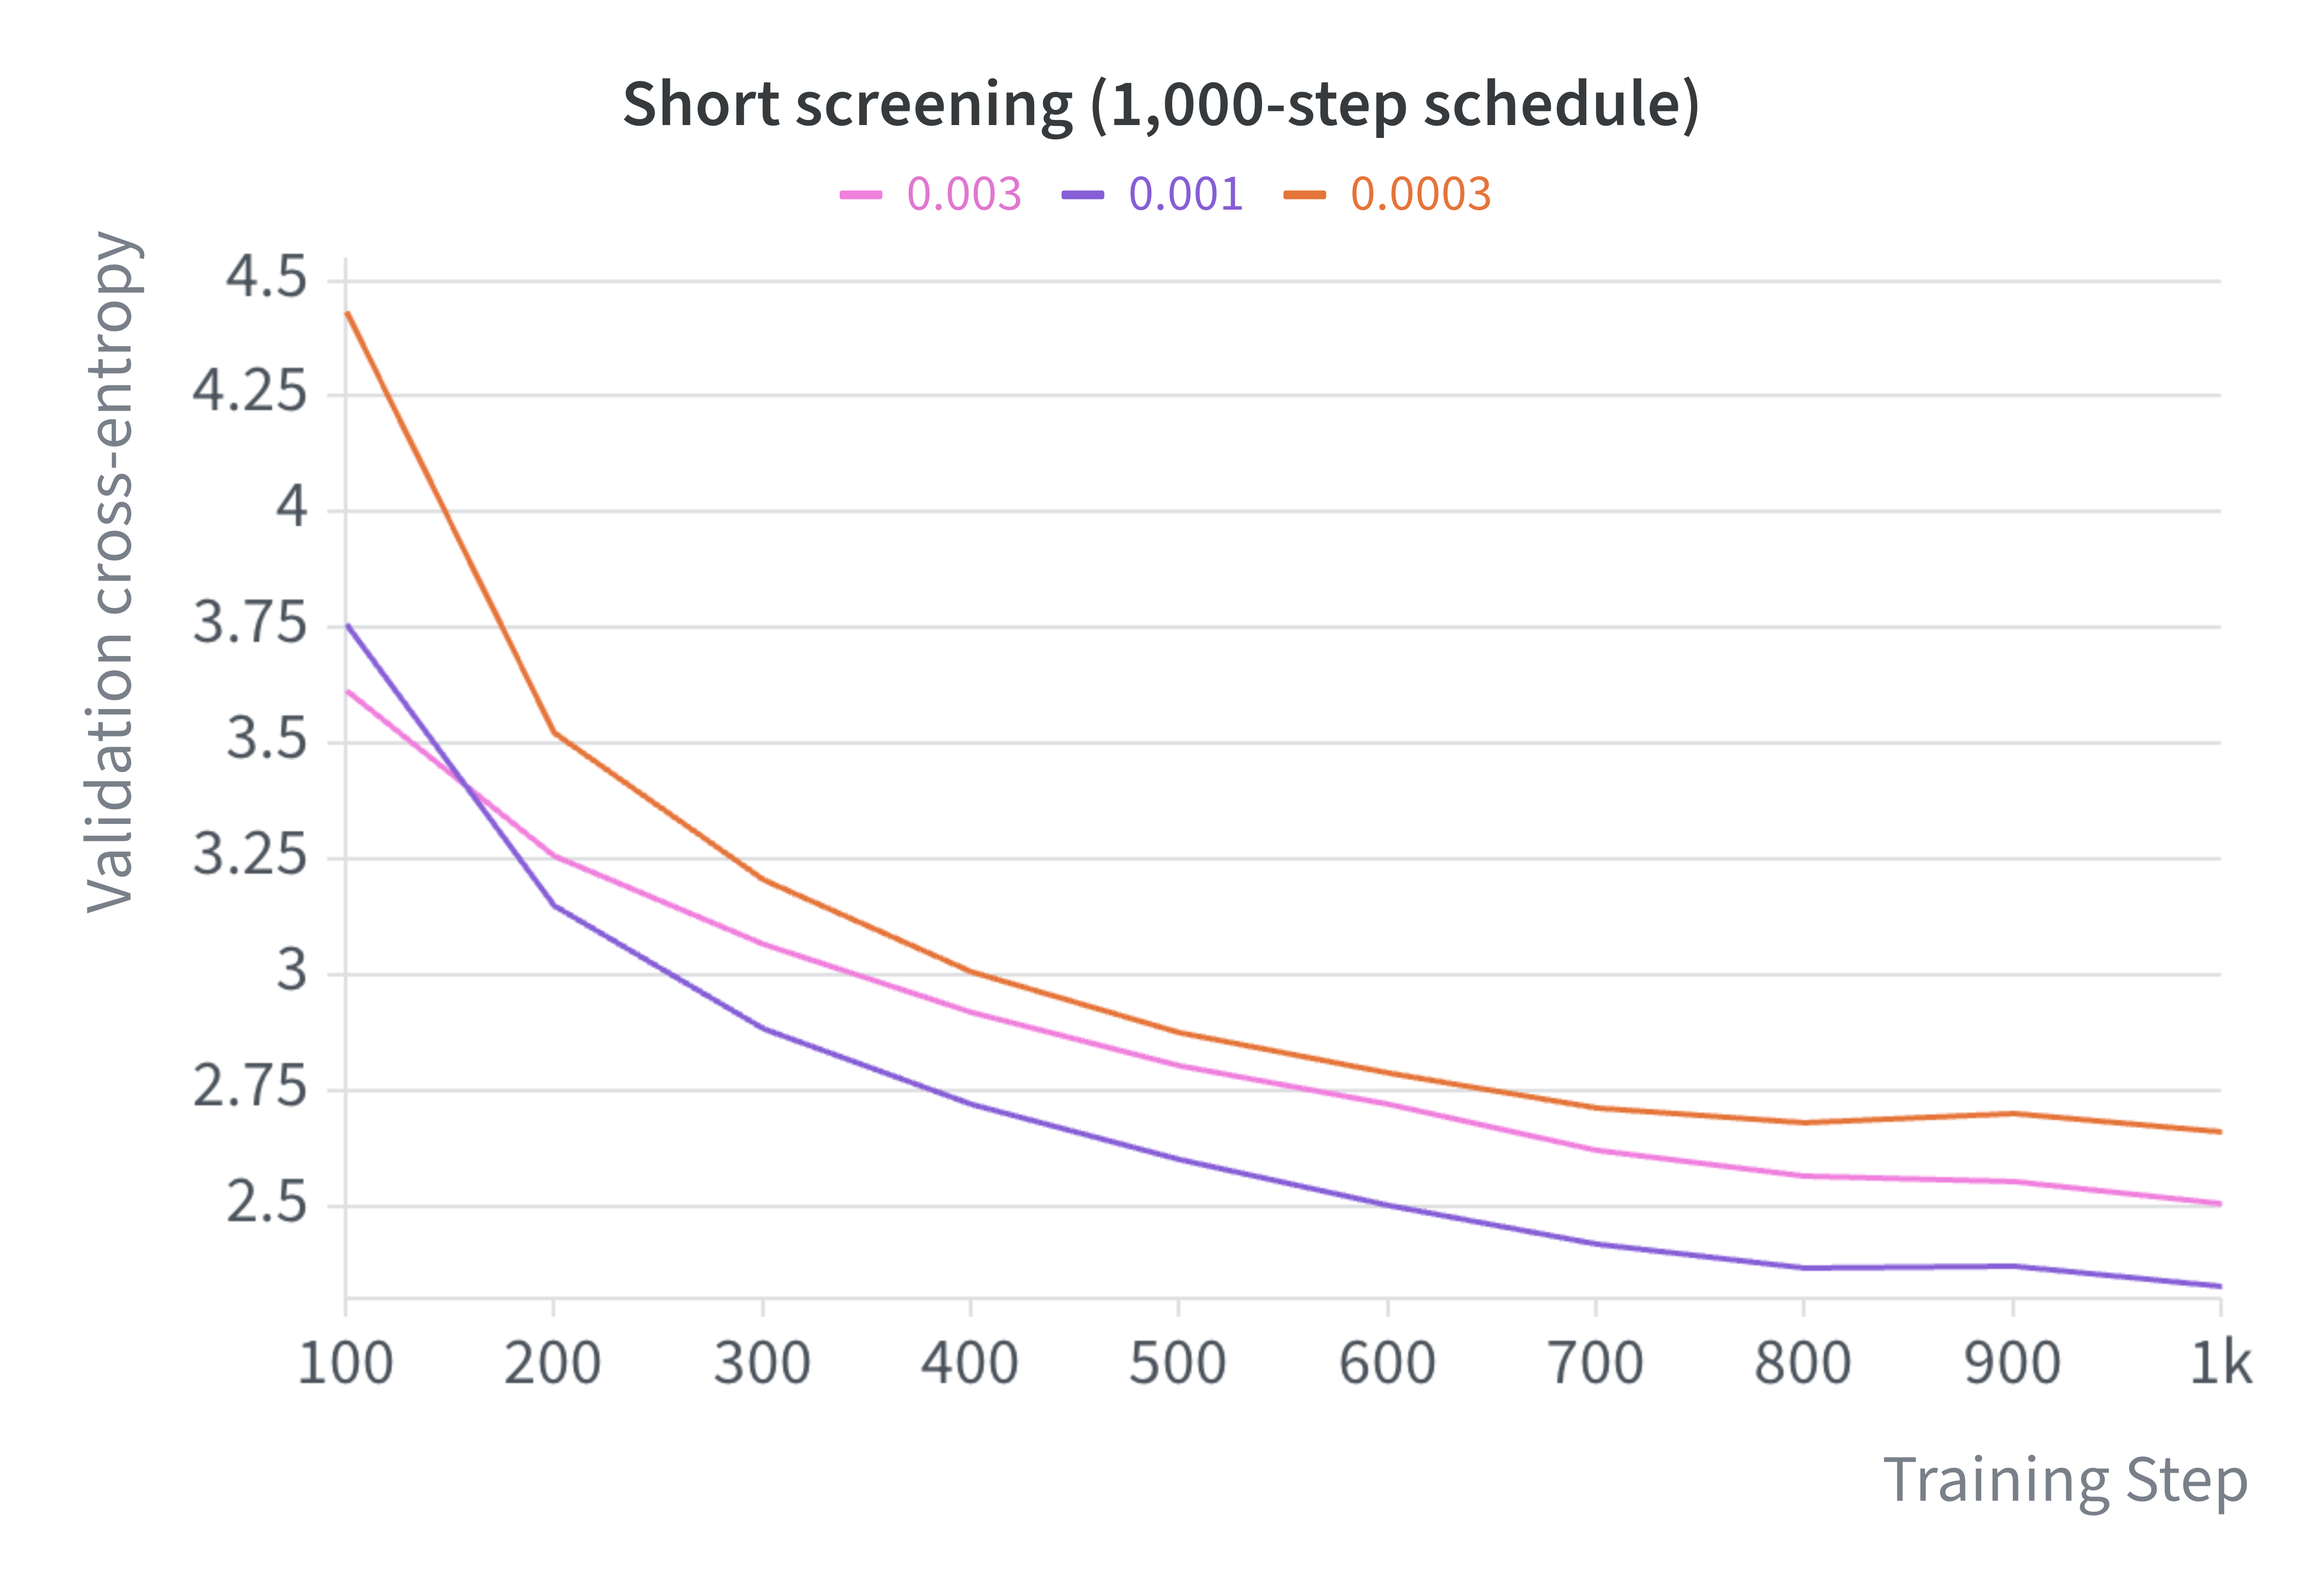
\includegraphics[width=0.49\textwidth]{figures/learning_rate_screening.png}\hfill
    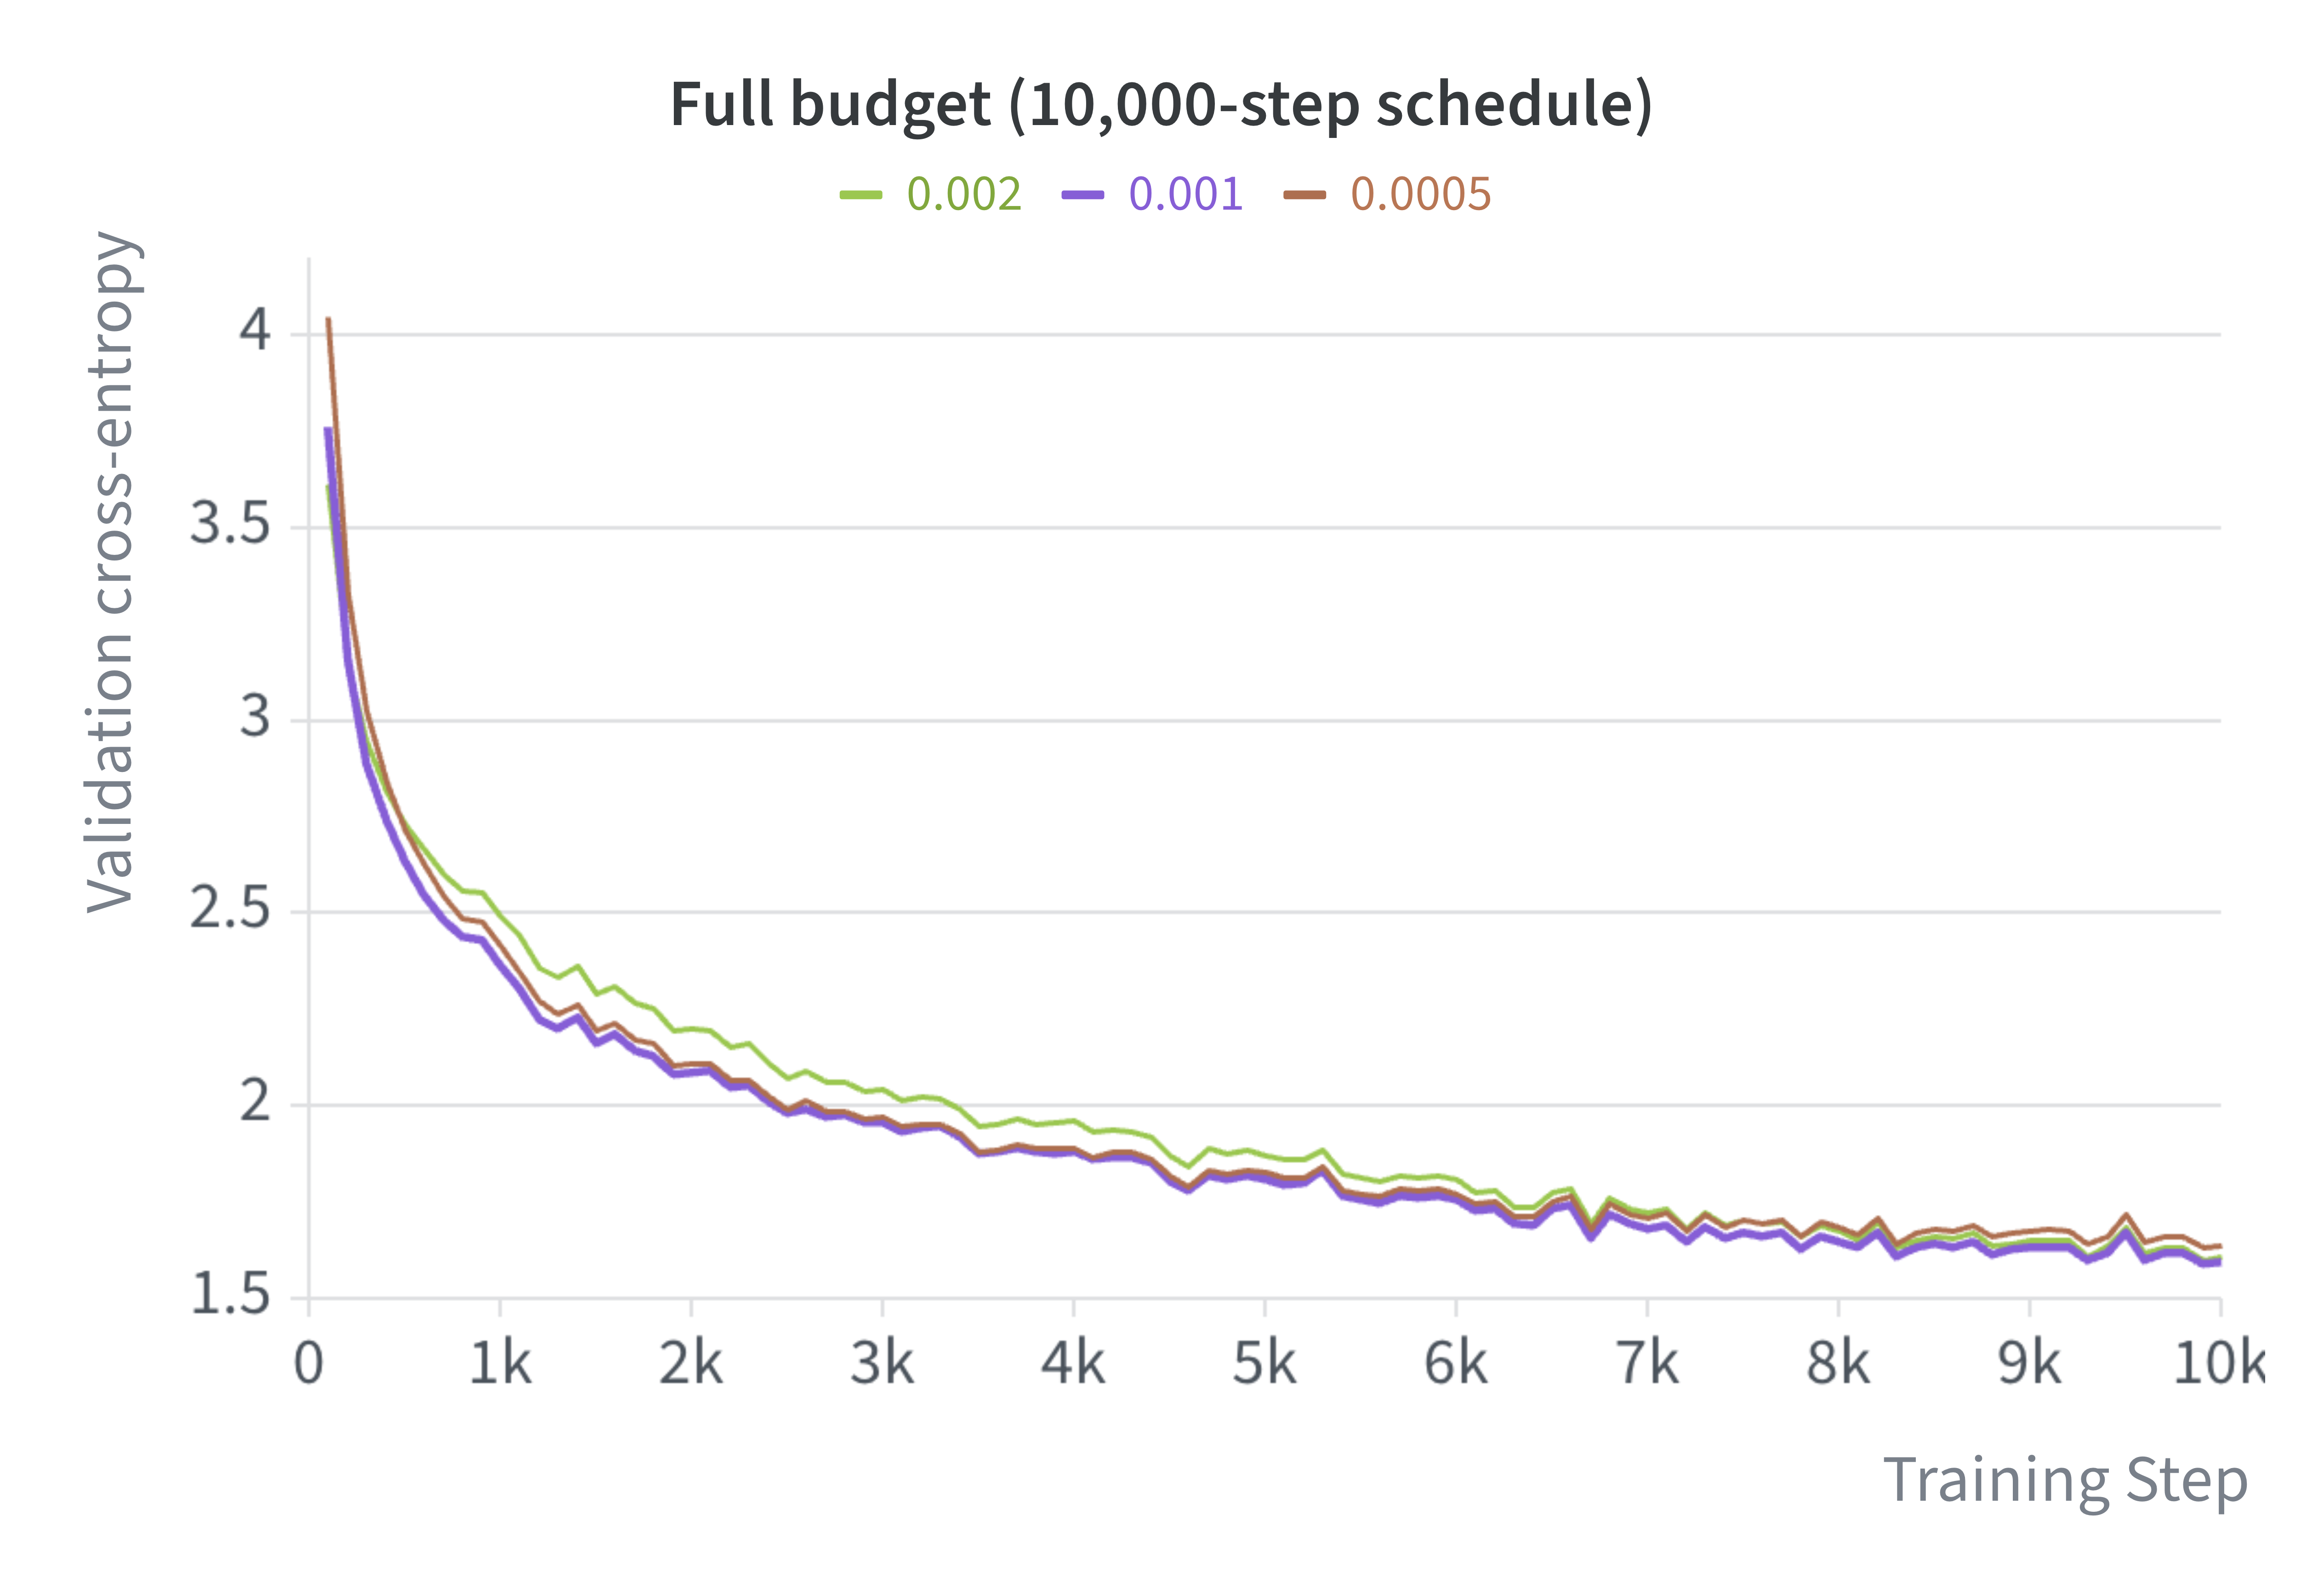
\includegraphics[width=0.49\textwidth]{figures/learning_rate_full_budget.png}
    \caption{W\&B validation curves for short screening (left) and
    full-budget comparisons (right), with smoothing disabled.
    Legends show peak learning rates. The low-resource validation target is 2.00.}
    \label{fig:lr_sweep}
\end{figure}

\begin{table}[H]
    \centering
    \small
    \begin{tabular}{@{}rrrrr@{}}
        \toprule
        Peak LR & Minimum LR & Final val loss & Best sampled val loss & Final PPL \\
        \midrule
        $5\times10^{-4}$ & $5\times10^{-5}$ & 1.6402 & 1.6343 & 5.16 \\
        $1\times10^{-3}$ & $1\times10^{-4}$ & \textbf{1.5966} & \textbf{1.5921} & \textbf{4.94} \\
        $2\times10^{-3}$ & $2\times10^{-4}$ & 1.6092 & 1.6010 & 5.00 \\
        \bottomrule
    \end{tabular}
    \caption{Equal-budget results after 10,000 steps (40.96M tokens).
    Final perplexity is $\exp(\text{final validation loss})$.}
    \label{tab:lr_results}
\end{table}

The best tested peak learning rate was $1\times10^{-3}$. It also had the lowest mean
validation loss over the last ten evaluations: 1.6188, compared with 1.6629
for $5\times10^{-4}$ and 1.6333 for $2\times10^{-3}$.
It outperformed these candidates at 100/100 and 98/100 corresponding evaluation
points, respectively. The final model reached validation loss 1.5966, meeting
the MPS low-resource target of 2.00; the best sampled loss was 1.5921 at step
9,900. I retained the final checkpoint and selected peak/minimum learning rates
$10^{-3}/10^{-4}$ for subsequent ablations. These are single-seed results over
three full-budget candidates, rather than evidence of a global optimum.

\newpage
\textbf{(b) High learning rates and stability.}

I increased the peak learning rate to $10^{-2}$, $3\times10^{-2}$, $10^{-1}$,
$0.3$, and $0.5$, keeping the other training settings fixed, including gradient
clipping. These fresh runs retained the 10,000-step cosine horizon and were
manually stopped at steps 1,040, 1,010, 1,080, 1,070, and 1,010, respectively.
Thus, these are early stability probes, not full-budget performance estimates.
Figure~\ref{fig:lr_divergence} compares their first 1,000 steps, during which
the post-warmup learning rates remained close to their peaks.

\begin{figure}[H]
    \centering
    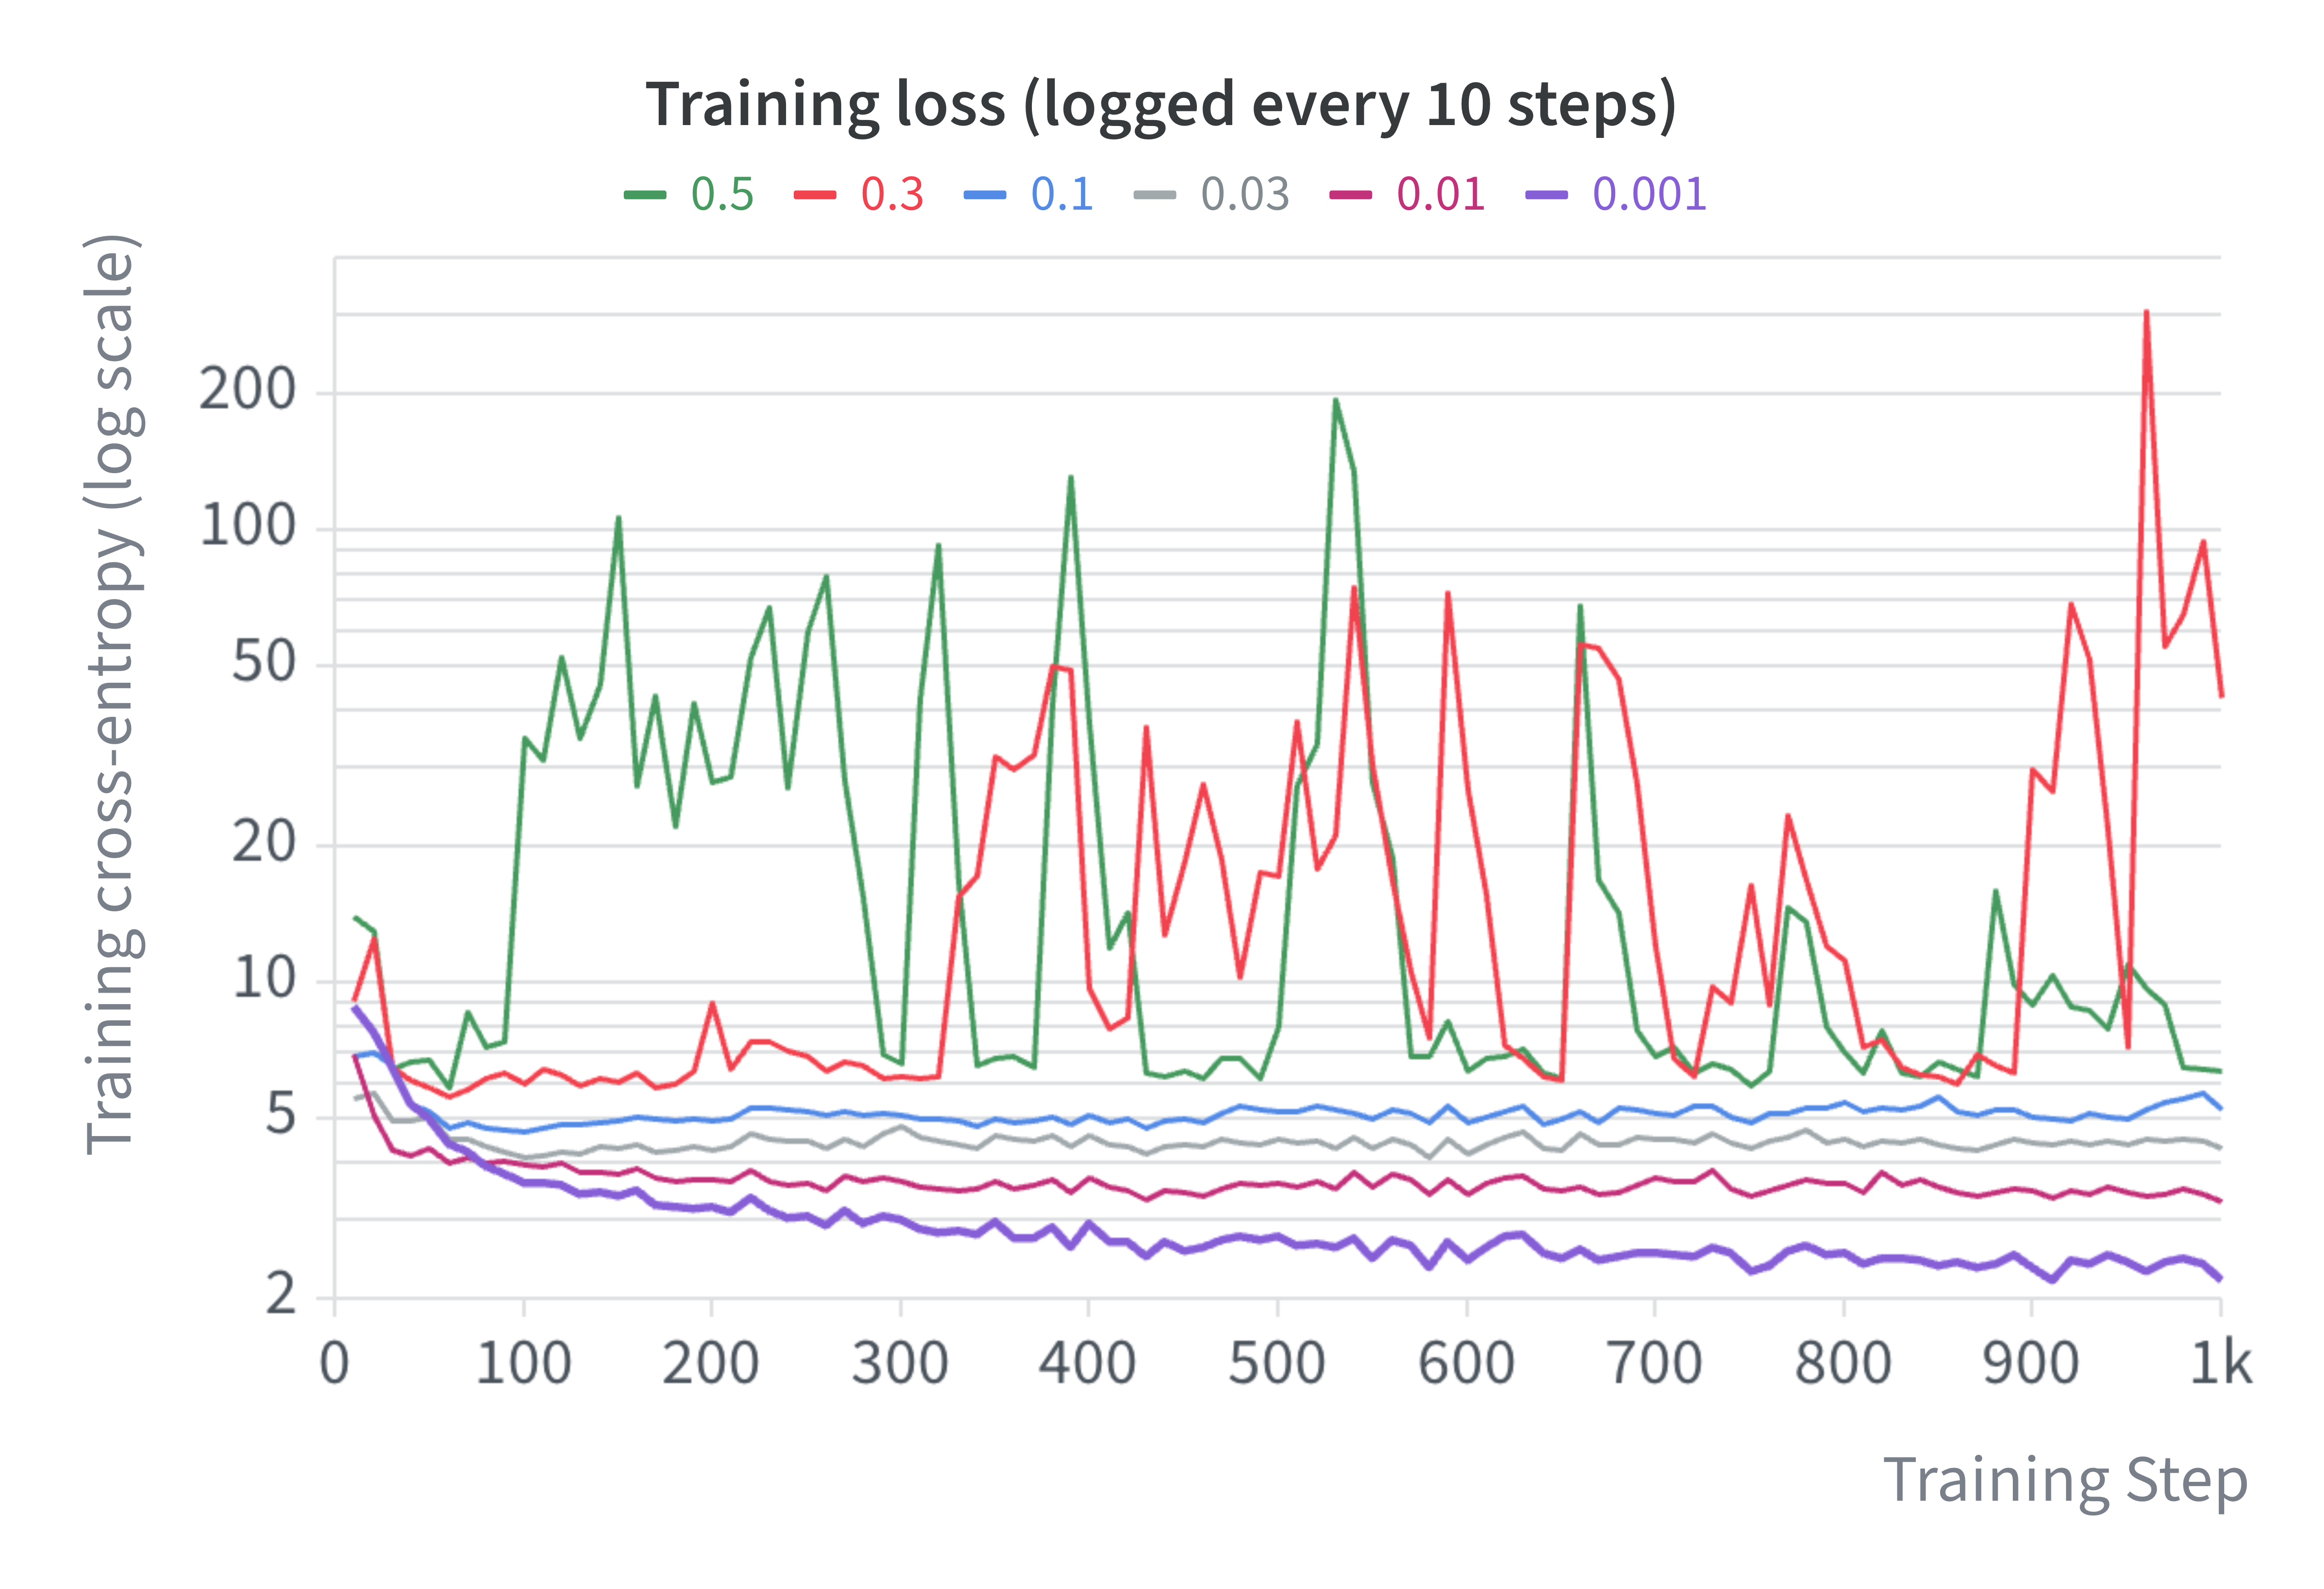
\includegraphics[width=0.49\textwidth]{figures/learning_rate_divergence_train.png}\hfill
    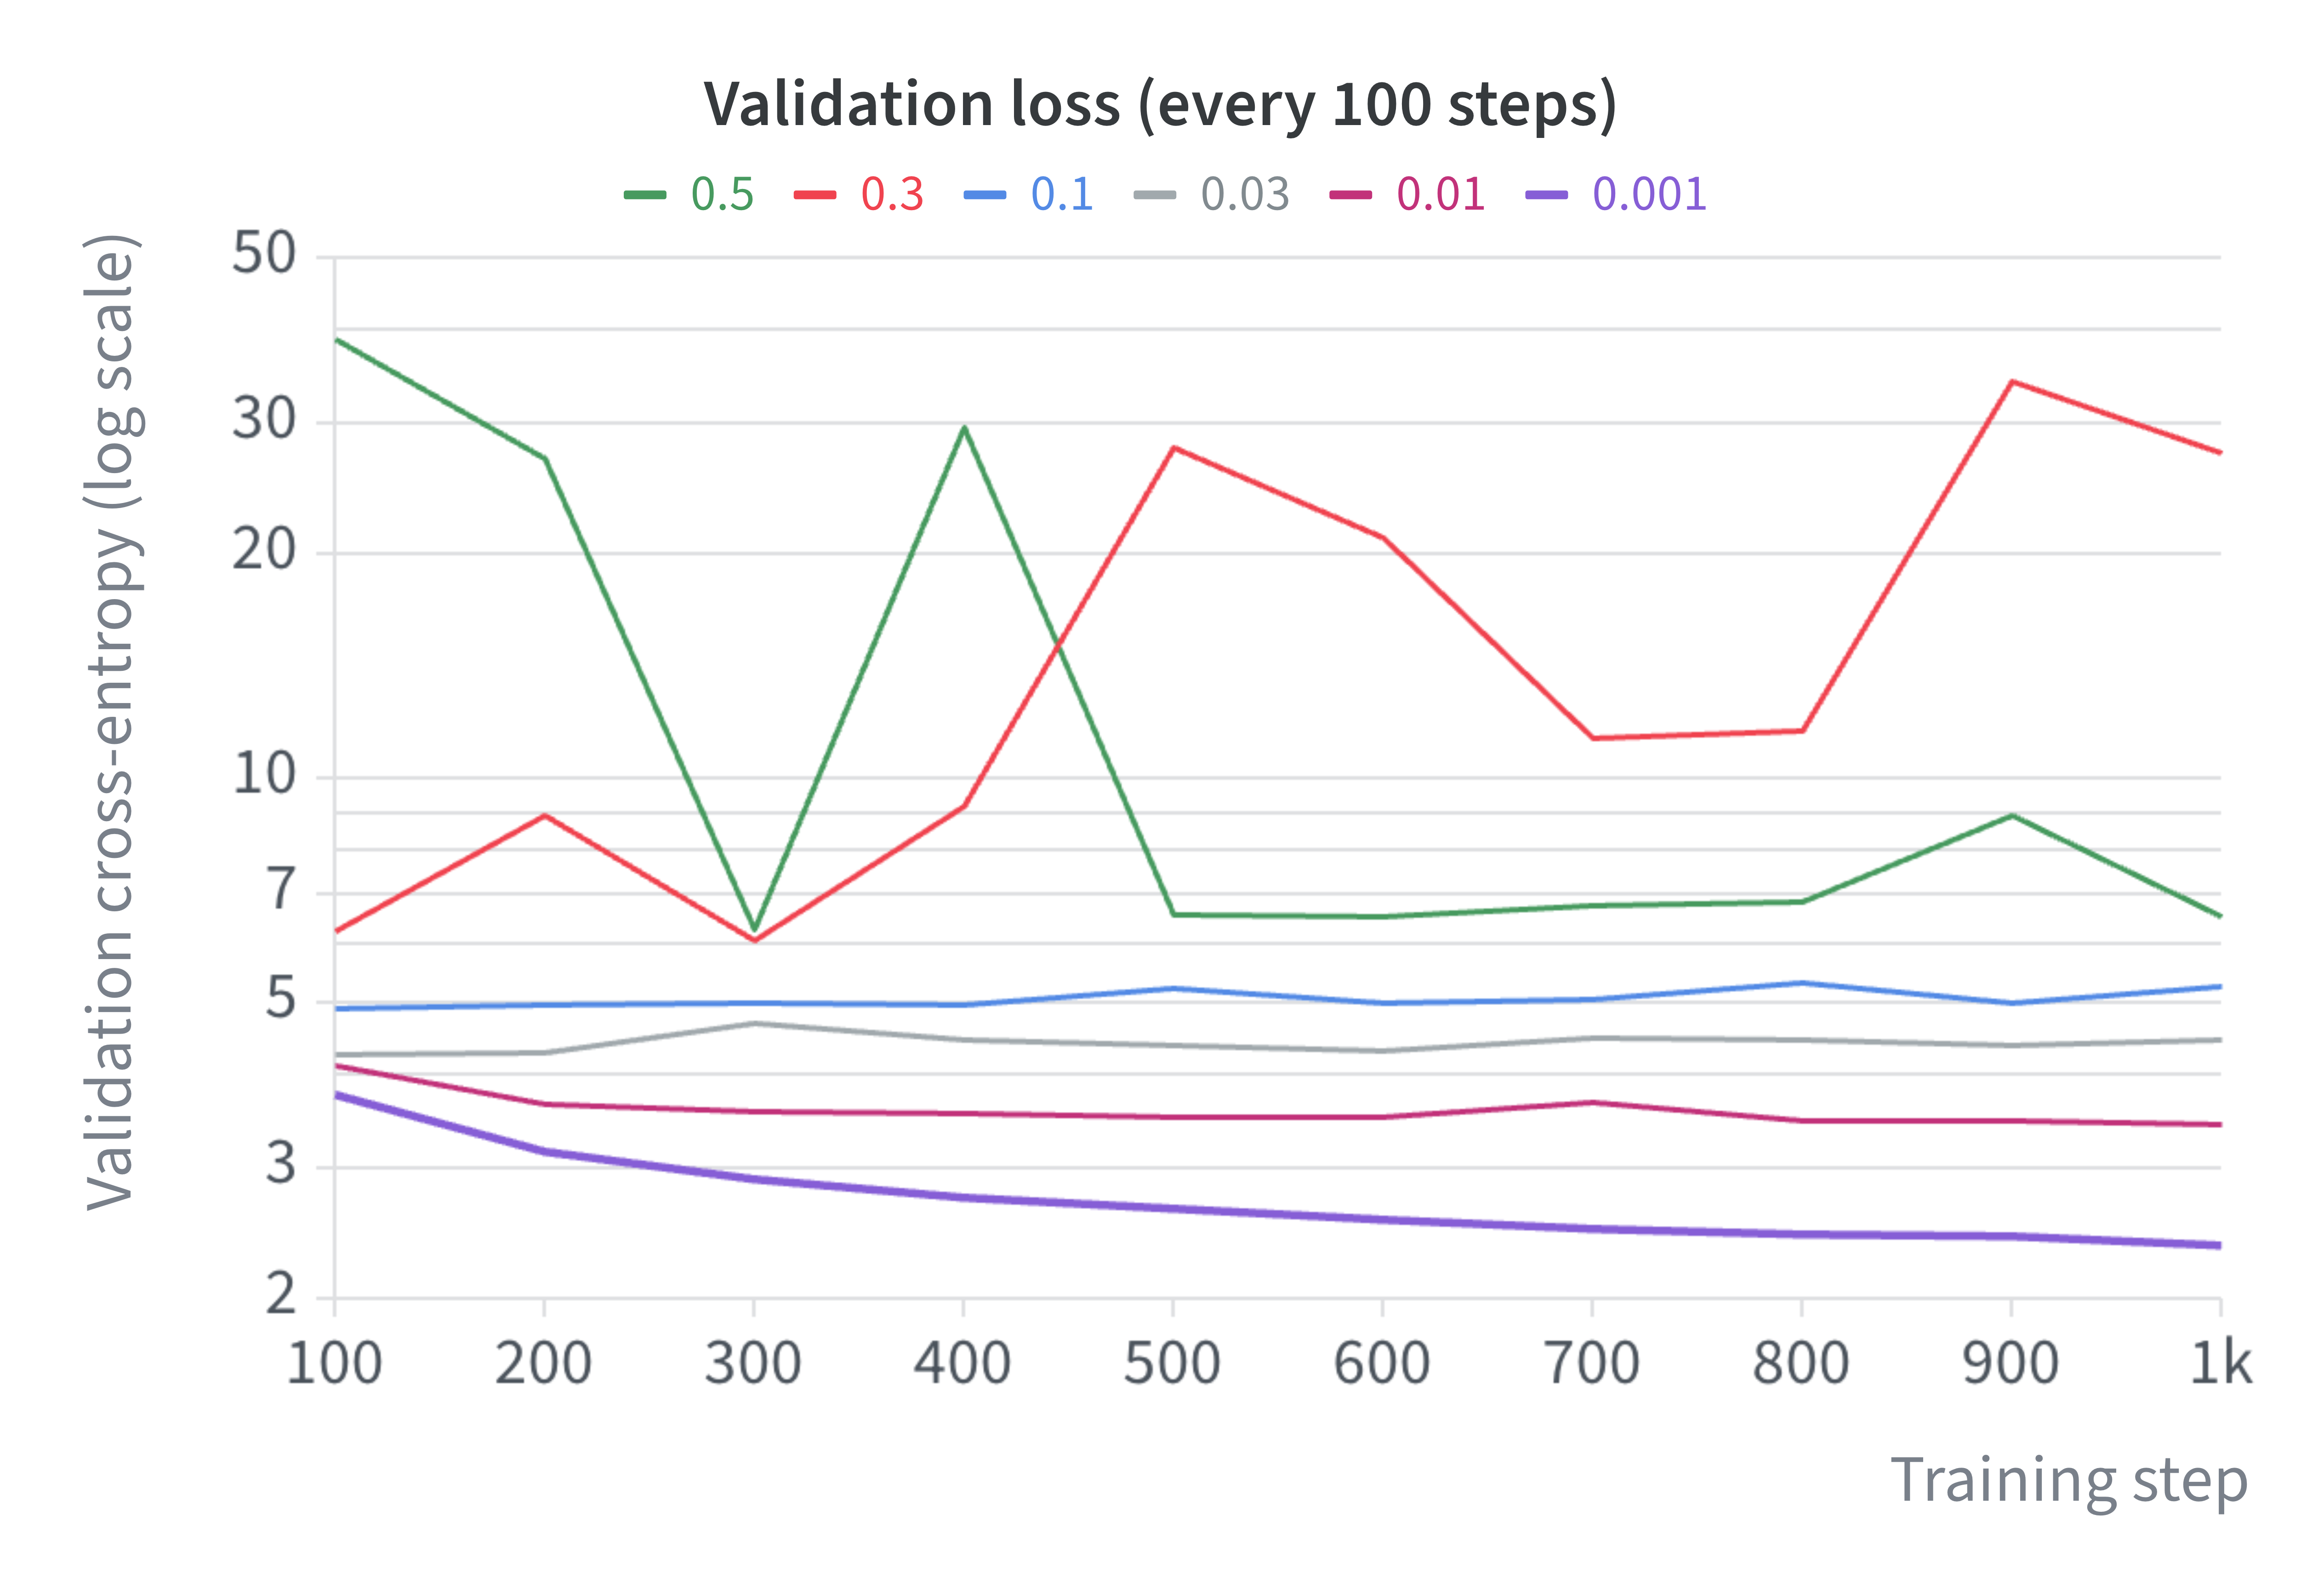
\includegraphics[width=0.49\textwidth]{figures/learning_rate_divergence_val.png}
    \caption{W\&B training (left) and validation (right) curves over the first
    1,000 steps, with smoothing disabled and logarithmic loss axes.
    Legends show peak learning rates; the $0.001$ curve is the full baseline
    restricted to this window. Warmup lasts 100 steps.}
    \label{fig:lr_divergence}
\end{figure}

\begin{table}[H]
    \centering
    \small
    \begin{tabular}{@{}rrl@{}}
        \toprule
        Peak LR & Val loss at step 1,000 & Observed behavior \\
        \midrule
        $10^{-3}$ & 2.3642 & Consistent improvement \\
        $10^{-2}$ & 3.4377 & Slow improvement \\
        $3\times10^{-2}$ & 4.4470 & High-loss plateau and oscillation \\
        $10^{-1}$ & 5.2528 & High-loss plateau and oscillation \\
        $0.3$ & 27.3223 & Repeated loss explosions \\
        $0.5$ & 6.5385 & Repeated loss explosions and recovery \\
        \bottomrule
    \end{tabular}
    \caption{High-LR probes compared at the same training step and token budget.}
    \label{tab:lr_stability}
\end{table}

The $10^{-2}$ run still learned, but much more slowly than the baseline;
$0.03$ and $0.1$ largely stalled. At $0.3$, training loss repeatedly exploded,
reaching a logged maximum of 305.5062 at step 960; validation loss reached
27.8814 at step 500 and 34.2393 at step 900.
At $0.5$, the logged training-loss maximum was 194.4761 at step 530, and
validation loss reached 38.9796 at step 100. These runs demonstrate optimization
divergence in the operational sense of repeated loss explosions and failure
to converge reliably. All logged values remained finite and losses sometimes
recovered: this is not evidence of NaN/Inf or monotonic, unbounded divergence.
The relatively low last validation loss for $0.5$ does not erase its earlier
instability.

In this search, increasing the learning rate beyond $10^{-3}$ did not accelerate
convergence: it first slowed learning and eventually caused severe instability.
The best full-budget candidate was well below the peaks showing loss explosions,
so these results do not support identifying it with a sharp ``edge of stability.''
The precise stability boundary was not located; the probes used one seed and
only about 1,000 steps, and the observed behavior depends on warmup, clipping,
and the other fixed settings.


\problem{batch\_size\_experiment}{Batch size variations}{1}

\deliverable{Learning curves for runs with different batch sizes.}

\begin{figure}[H]
    \centering
    % \includegraphics[width=0.8\textwidth]{figures/batch_size_experiment.png}
    \fbox{\parbox{0.8\textwidth}{\centering\vspace{2cm} Batch size experiment learning curves \\ \textit{(insert figure here)}\vspace{2cm}}}
    \caption{Learning curves for different batch sizes on TinyStories.}
    \label{fig:batch_size}
\end{figure}

\deliverable{A few sentences discussing your findings on batch sizes and their impacts on training.}

\textit{Findings:} % TODO: your findings


\problem{generate}{Generate text}{1}

\deliverable{Text dump of at least 256 tokens of text (or until the first \texttt{<eos>} token), and a brief comment on fluency.}

\textbf{Setup.} We used the final TinyStories baseline checkpoint trained
for 10,000 updates at batch size 16 (40.96M tokens), with peak/floor learning
rates $10^{-3}/10^{-4}$. Generation used MPS, seed 42, top-$p=0.9$, and a
limit of 256 new tokens, stopping earlier if EOS was sampled. The CLI omits
the terminal EOS from the displayed text. The prompt, checkpoint, seed, and
top-$p$ were fixed while temperature varied across $0.7$, $1.0$, and $1.3$.
Each text below includes the prompt.

\textbf{Generated text, temperature $0.7$.}
\begin{quote}
Once upon a time, there was a little girl named Lily. She loved to play outside in the snow. One day, she saw a big, pretty flower that was blooming in the sun. Lily thought the flower was very pretty.

Lily wanted to show her friends the flower. She took a big step and danced around. She saw her friends, the bees, and the bees. They all danced together, and Lily felt happy.

But then, a mean fox came to the garden. The fox wanted to take the flower from Lily and her friends. The fox was not nice to take the flower. He took the flower and ran away. Lily was sad and cried. She went back to her friends and told them about the fox. They all learned to be careful with the pretty flower and not let it hurt them.
\end{quote}

\textbf{Generated text, temperature $1.0$.}
\begin{quote}
Once upon a time, there was a little girl named Lily. She loved to play outside in the snow. One day, she saw a unique triangle in the snow. It was big and round. Lily was very happy and excited to play with it.

Lily picked up the triangle and put it on the ground. She played with it all day long. When it was time to go inside, she was tired but happy. So, she put the triangle in the snow and went inside to have some hot cocoa.

While she was outside, the unique triangle was starting to melt. It got bigger and bigger, and the triangle felt sad. Lily sat down under the snow and laughed. The triangle's face was gone, and the cone was gone.

From that day on, Lily and the unique triangle had many more fun playing in the snow. They made snow angels, even when it rained. And they always played in the snow together.
\end{quote}

\textbf{Generated text, temperature $1.3$.}
\begin{quote}
Once upon a time, there was a little girl named Lily. She loved to ask her mom to make some shampoo. One day, it was spoiled and was all one fun hair she could do.

Lily's mom told her to put a new red thread around like a lamp one by one. She said it would keep blue again, so Lily could have eleven wheel parties at once.

So every day. When the heel from put over all of the facereenening sizes of first, why hard about it now? But Lily resisted admiring it! They clapped for her, and she was so happy. She was able to put the oil over it every day.
\end{quote}

\textbf{Fluency and sampling.} Of these three samples, temperature $0.7$
produced the most coherent story and mostly grammatical sentences. However,
it repeated ``the bees'' and ended with a moral weakly connected to the plot.
At $1.0$, many sentences remained locally fluent, but the triangle was
described as round, grew while melting, and was followed by an unexplained
cone. At $1.3$, grammatical errors, unrelated phrases, and the malformed word
``facereenening'' made the story difficult to follow.

Two factors affect output quality. First, temperature changes the sampling
distribution: increasing it gives lower-probability tokens more weight,
potentially increasing variety while also admitting errors. Top-$p$ further
restricts the candidate set; it was held fixed here, so its effect was not
measured separately. Second, the learned model distribution matters: this
40.96M-token model can produce familiar story structures but still exhibits
repetition, semantic contradictions, and weak long-range consistency even at
the lowest tested temperature. The observed temperature ranking applies to
this prompt and seed; it does not establish a generally optimal temperature.

\FloatBarrier
\newpage
\problem{layer\_norm\_ablation}{Remove RMSNorm and train}{1}

\textbf{Common protocol for the four ablations.}
I used TinyStories and the low-resource configuration: vocabulary 10,000,
context length 256, four layers, width 512, 16 heads, and batch size 16.
Each full run started from scratch with seed 42 and trained for 10,000 updates
(40.96M tokens) on MPS. AdamW used $\beta=(0.9,0.999)$, weight decay 0.1,
and gradient clipping at 1.0. After 100 warmup updates, the learning rate
followed cosine decay from $10^{-3}$ to $10^{-4}$, except for the reduced-LR
no-RMSNorm run described below. The baseline used pre-RMSNorm, RoPE, and
SwiGLU with hidden width 1,344.

For these comparisons I trained a fresh baseline and evaluated every 100
updates on the same 20 batches of 16 validation windows (81,920 tokens),
using a private generator reset to seed 42 at each evaluation. Validation
therefore did not consume the training sampler's random state. This protocol
differs from the earlier LR sweep's random validation sampling, so I use the
new baseline throughout this section rather than directly comparing its loss
with the older baseline. Figures are exported from W\&B panels with smoothing disabled.
Training loss is the current minibatch loss logged every ten updates;
validation loss uses the fixed windows described above.
All five full runs completed with finite logged losses and finite final model
weights; their final checkpoints also gave their best sampled validation losses.

\begin{table}[H]
    \centering
    \small
    \begin{tabular}{@{}lrrrr@{}}
        \toprule
        Model & Peak LR & Parameters & Final val loss & $\Delta$ vs. baseline \\
        \midrule
        Baseline & $10^{-3}$ & 22,696,448 & \textbf{1.5879} & --- \\
        No RMSNorm & $5\times10^{-4}$ & 22,691,840 & 1.6598 & $+0.0719$ \\
        Post-norm & $10^{-3}$ & 22,696,448 & 1.6042 & $+0.0163$ \\
        NoPE & $10^{-3}$ & 22,696,448 & 1.7010 & $+0.1131$ \\
        SiLU & $10^{-3}$ & 22,827,520 & 1.6106 & $+0.0227$ \\
        \bottomrule
    \end{tabular}
    \caption{Matched-budget ablation results at step 10,000. Lower validation
    cross-entropy is better. All runs use one seed; no-RMSNorm also changes LR.}
    \label{tab:ablation_results}
\end{table}

\textbf{Removing normalization and selecting a learning rate.}
I removed every RMSNorm, including the final normalization before the output
projection. At the previously selected peak LR $10^{-3}$, an early probe
with the 10,000-step schedule became unstable: validation loss reached 7.4620
at update 300 and 2125.2192 at update 400, before recovering to 2.4755 at
update 1,000. The values remained finite; this was a transient loss explosion,
not persistent unbounded divergence. This probe was stopped early and is not
a full-budget result.

I then screened peaks $3\times10^{-4}$ and $5\times10^{-4}$ with the same
long schedule. Neither showed comparable spikes in the logged window;
$5\times10^{-4}$ had lower loss at all ten corresponding evaluations,
ending at 2.4873 versus 2.5967 at update 1,000. I selected
$5\times10^{-4}$ with floor $5\times10^{-5}$ for a fresh full run.
This is the selected stable candidate among the short screens, rather than
a proven full-budget optimum.

\begin{figure}[H]
    \centering
    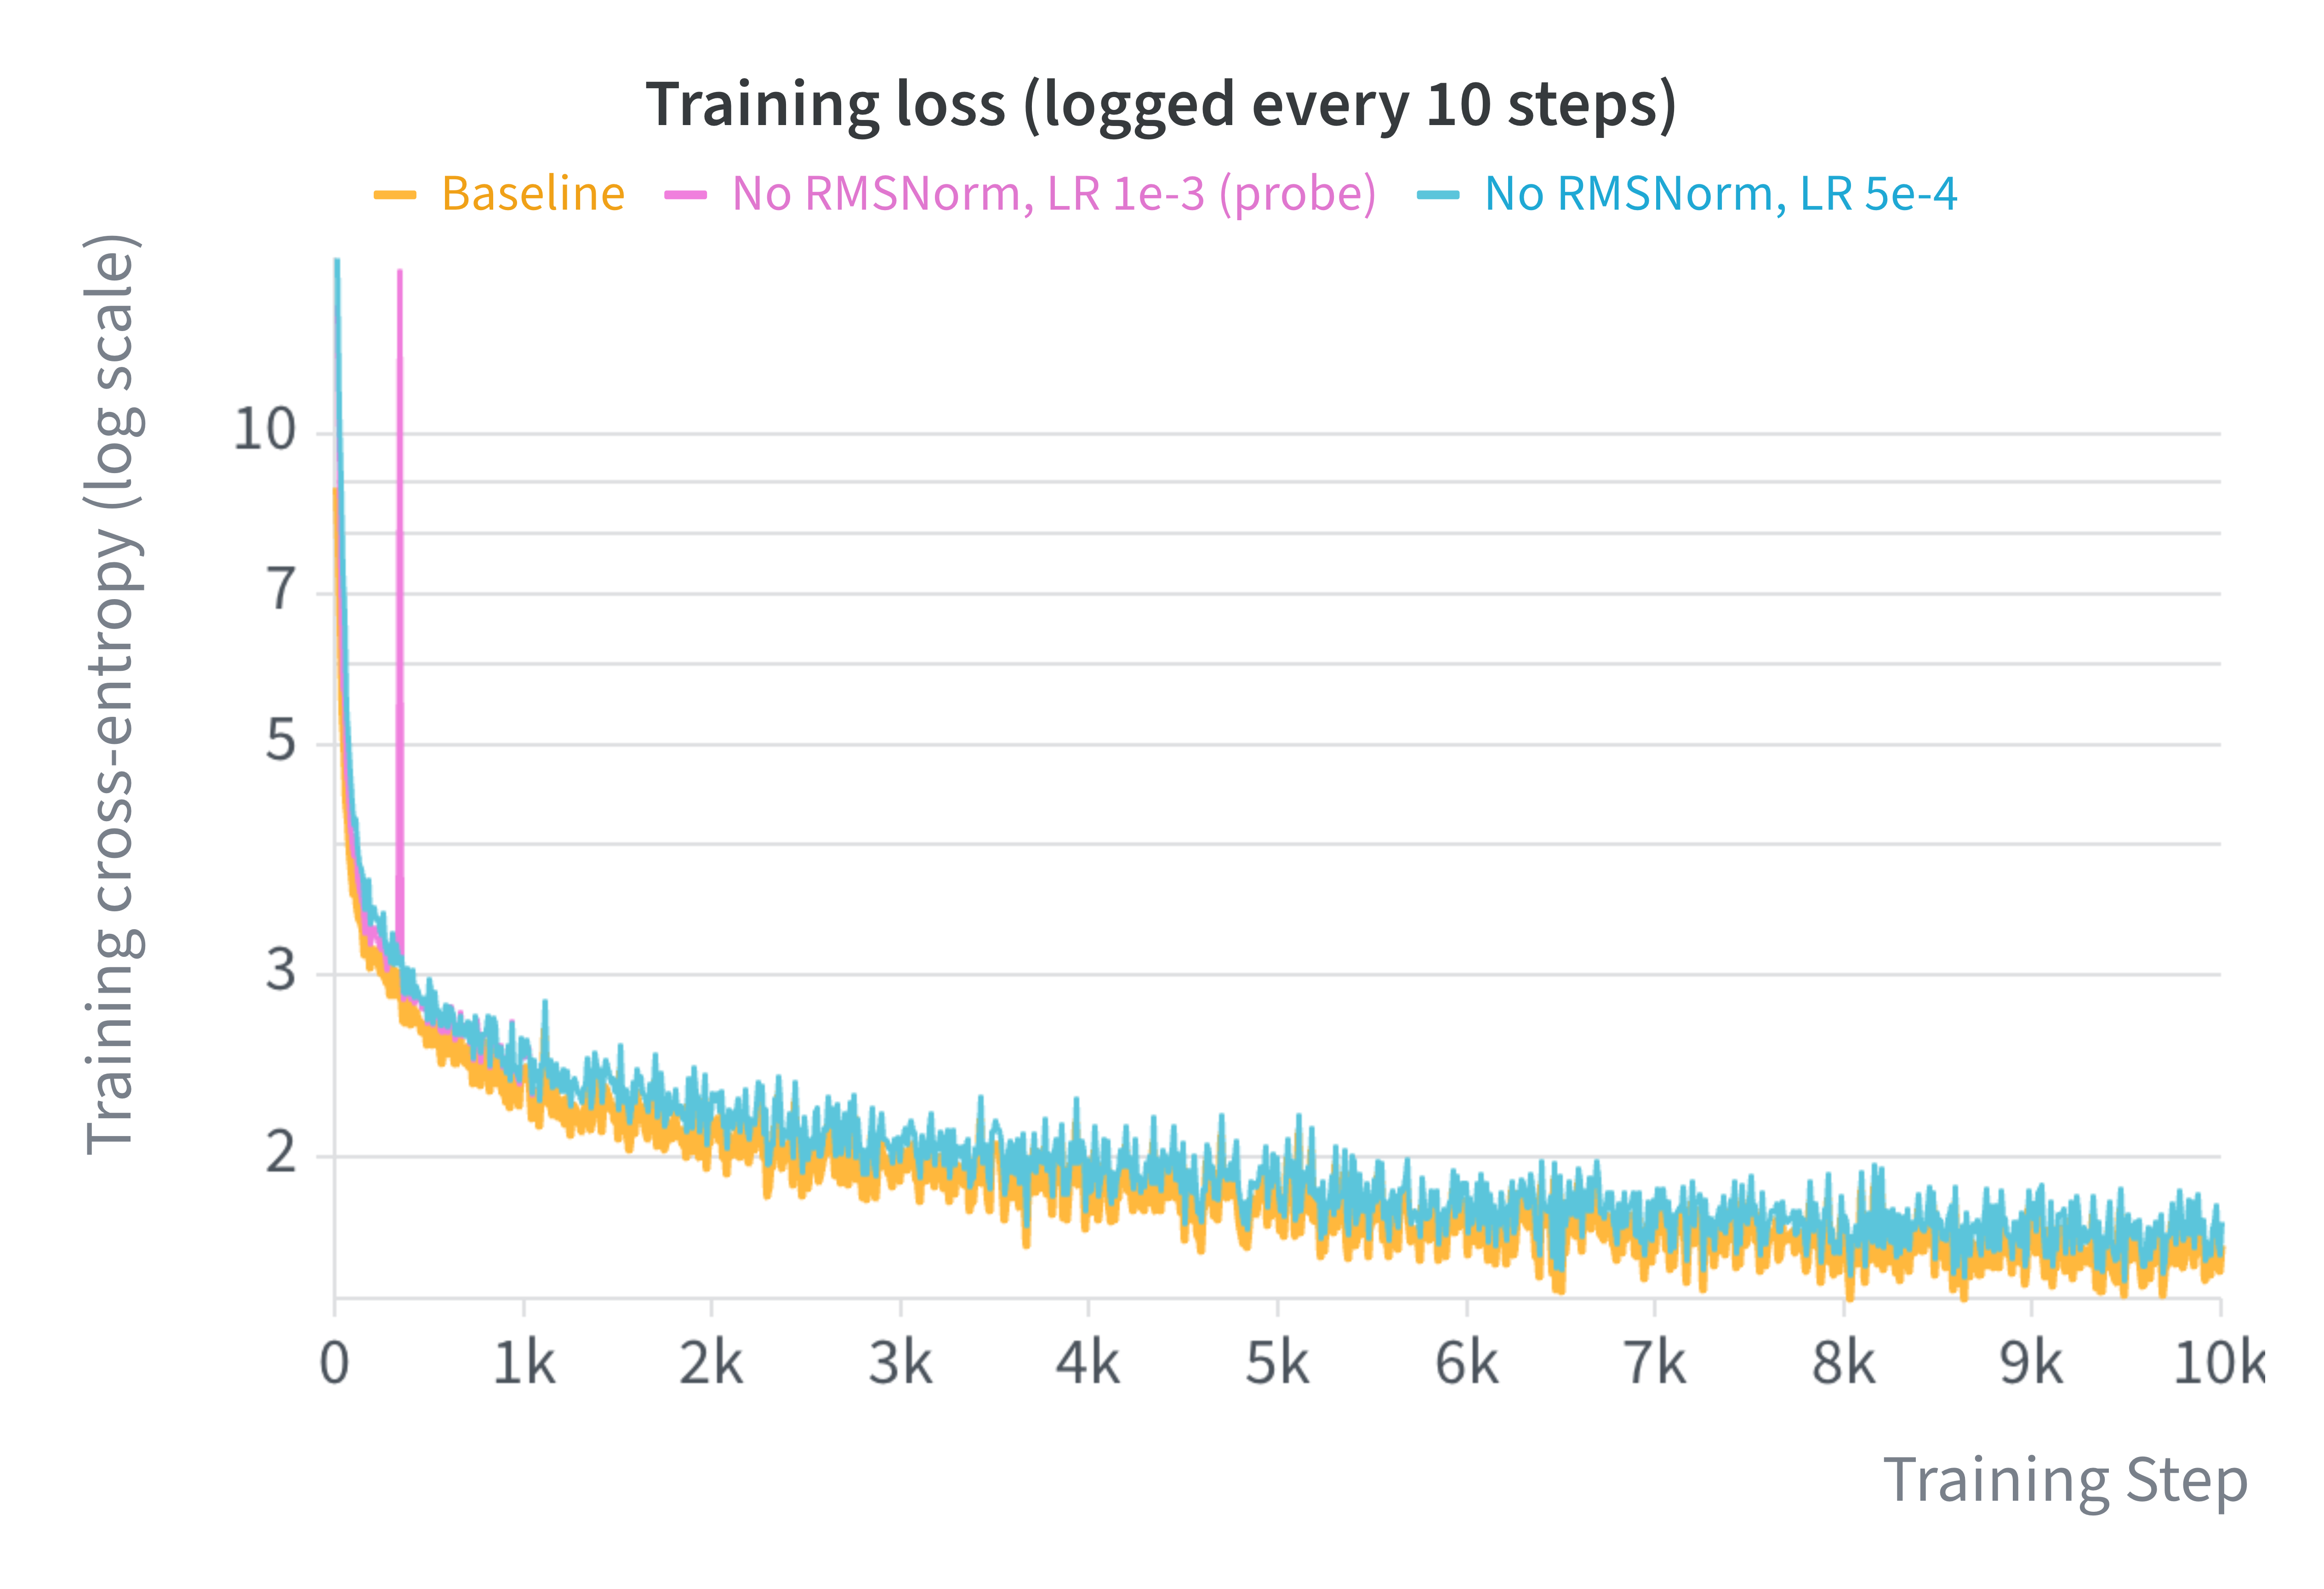
\includegraphics[width=0.49\textwidth]{figures/rmsnorm_train.png}\hfill
    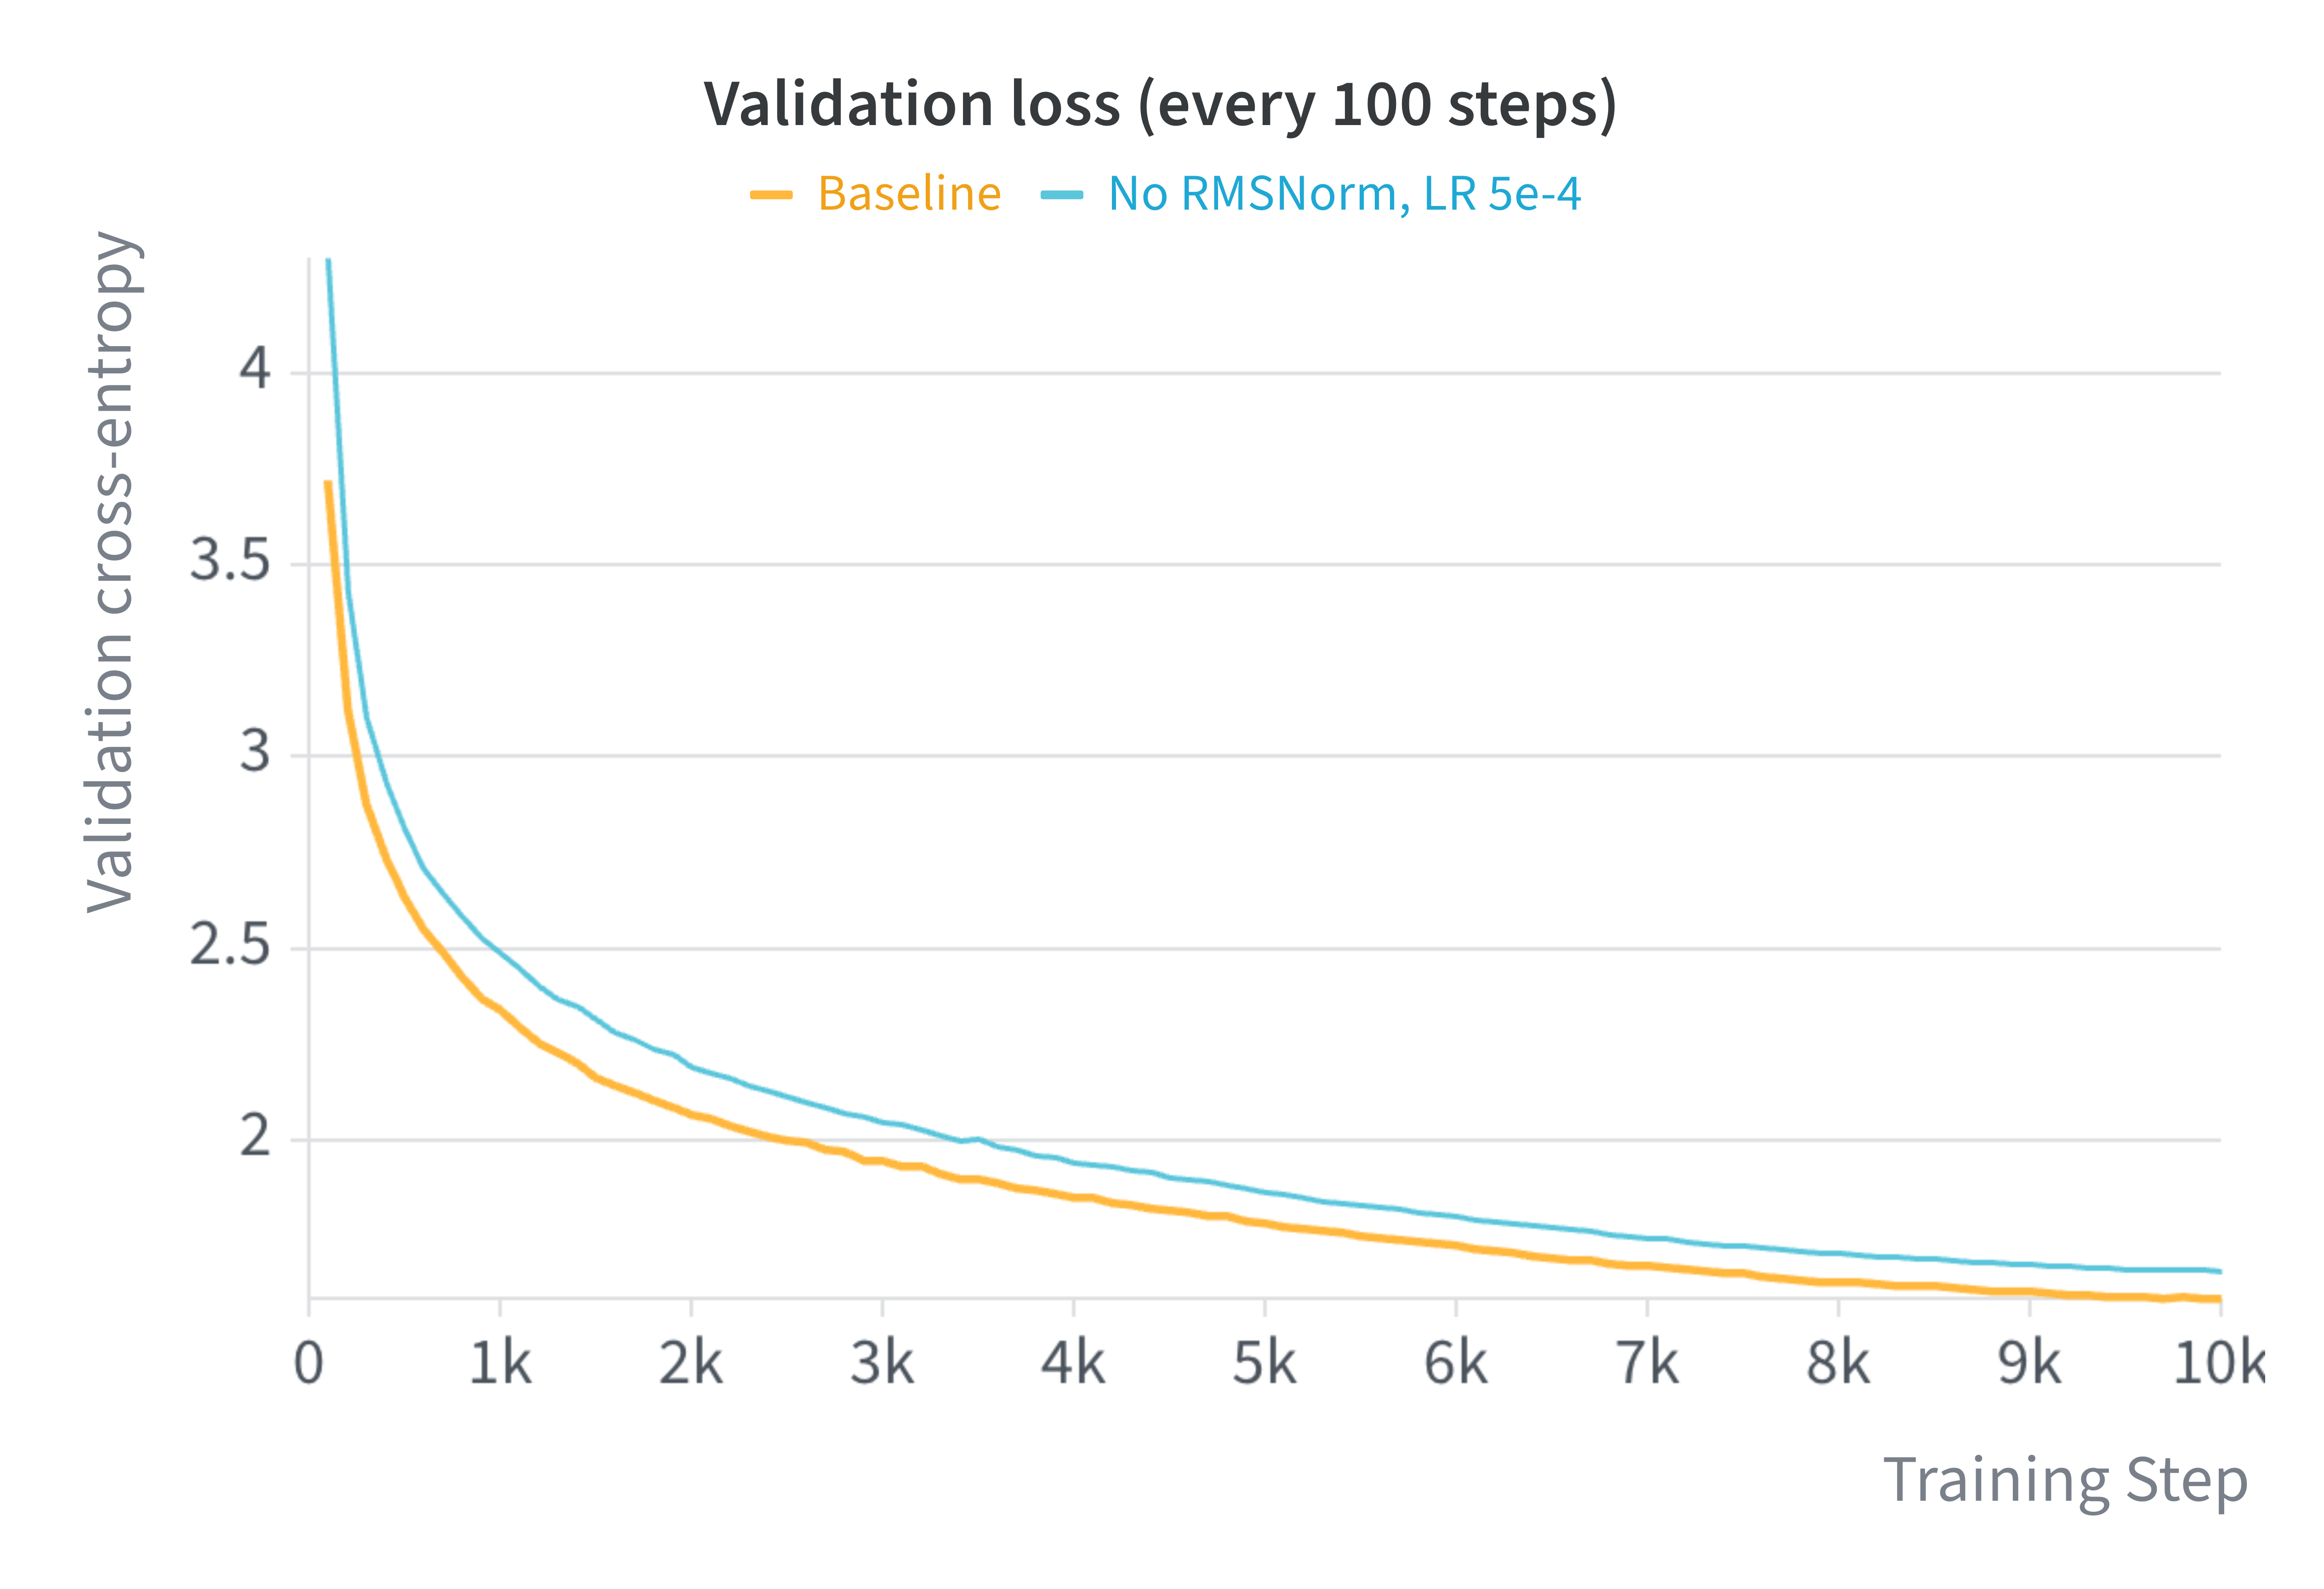
\includegraphics[width=0.49\textwidth]{figures/rmsnorm_val.png}
    \caption{RMSNorm ablation: W\&B training loss (left, logarithmic loss axis)
    and validation loss (right, linear loss axis). The training panel includes
    the early $10^{-3}$ no-RMSNorm probe, which ends near update 1,000;
    the validation panel compares only the complete baseline and reduced-LR
    no-RMSNorm runs. Legends give peak LR; floors are one tenth of peak.}
    \label{fig:layer_norm_ablation}
\end{figure}

The reduced-LR full run remained stable at the logged evaluations and reached
1.6598, compared with 1.5879 for the baseline. Its validation loss was higher
at all 100 matched evaluation points. Thus, normalization allowed stable
training at the larger tested LR, while reducing LR made training without
normalization practical in this setting. The final gap of 0.0719 reflects
both the architecture and the different LR schedule; it does not isolate the
causal effect of RMSNorm alone.

\newpage
\problem{pre\_norm\_ablation}{Implement post-norm and train}{1}

I moved each block's two RMSNorms after its attention and feed-forward
residual additions, retaining the final model RMSNorm. Model size, learning
rate, and the remaining common settings were unchanged.

\begin{figure}[H]
    \centering
    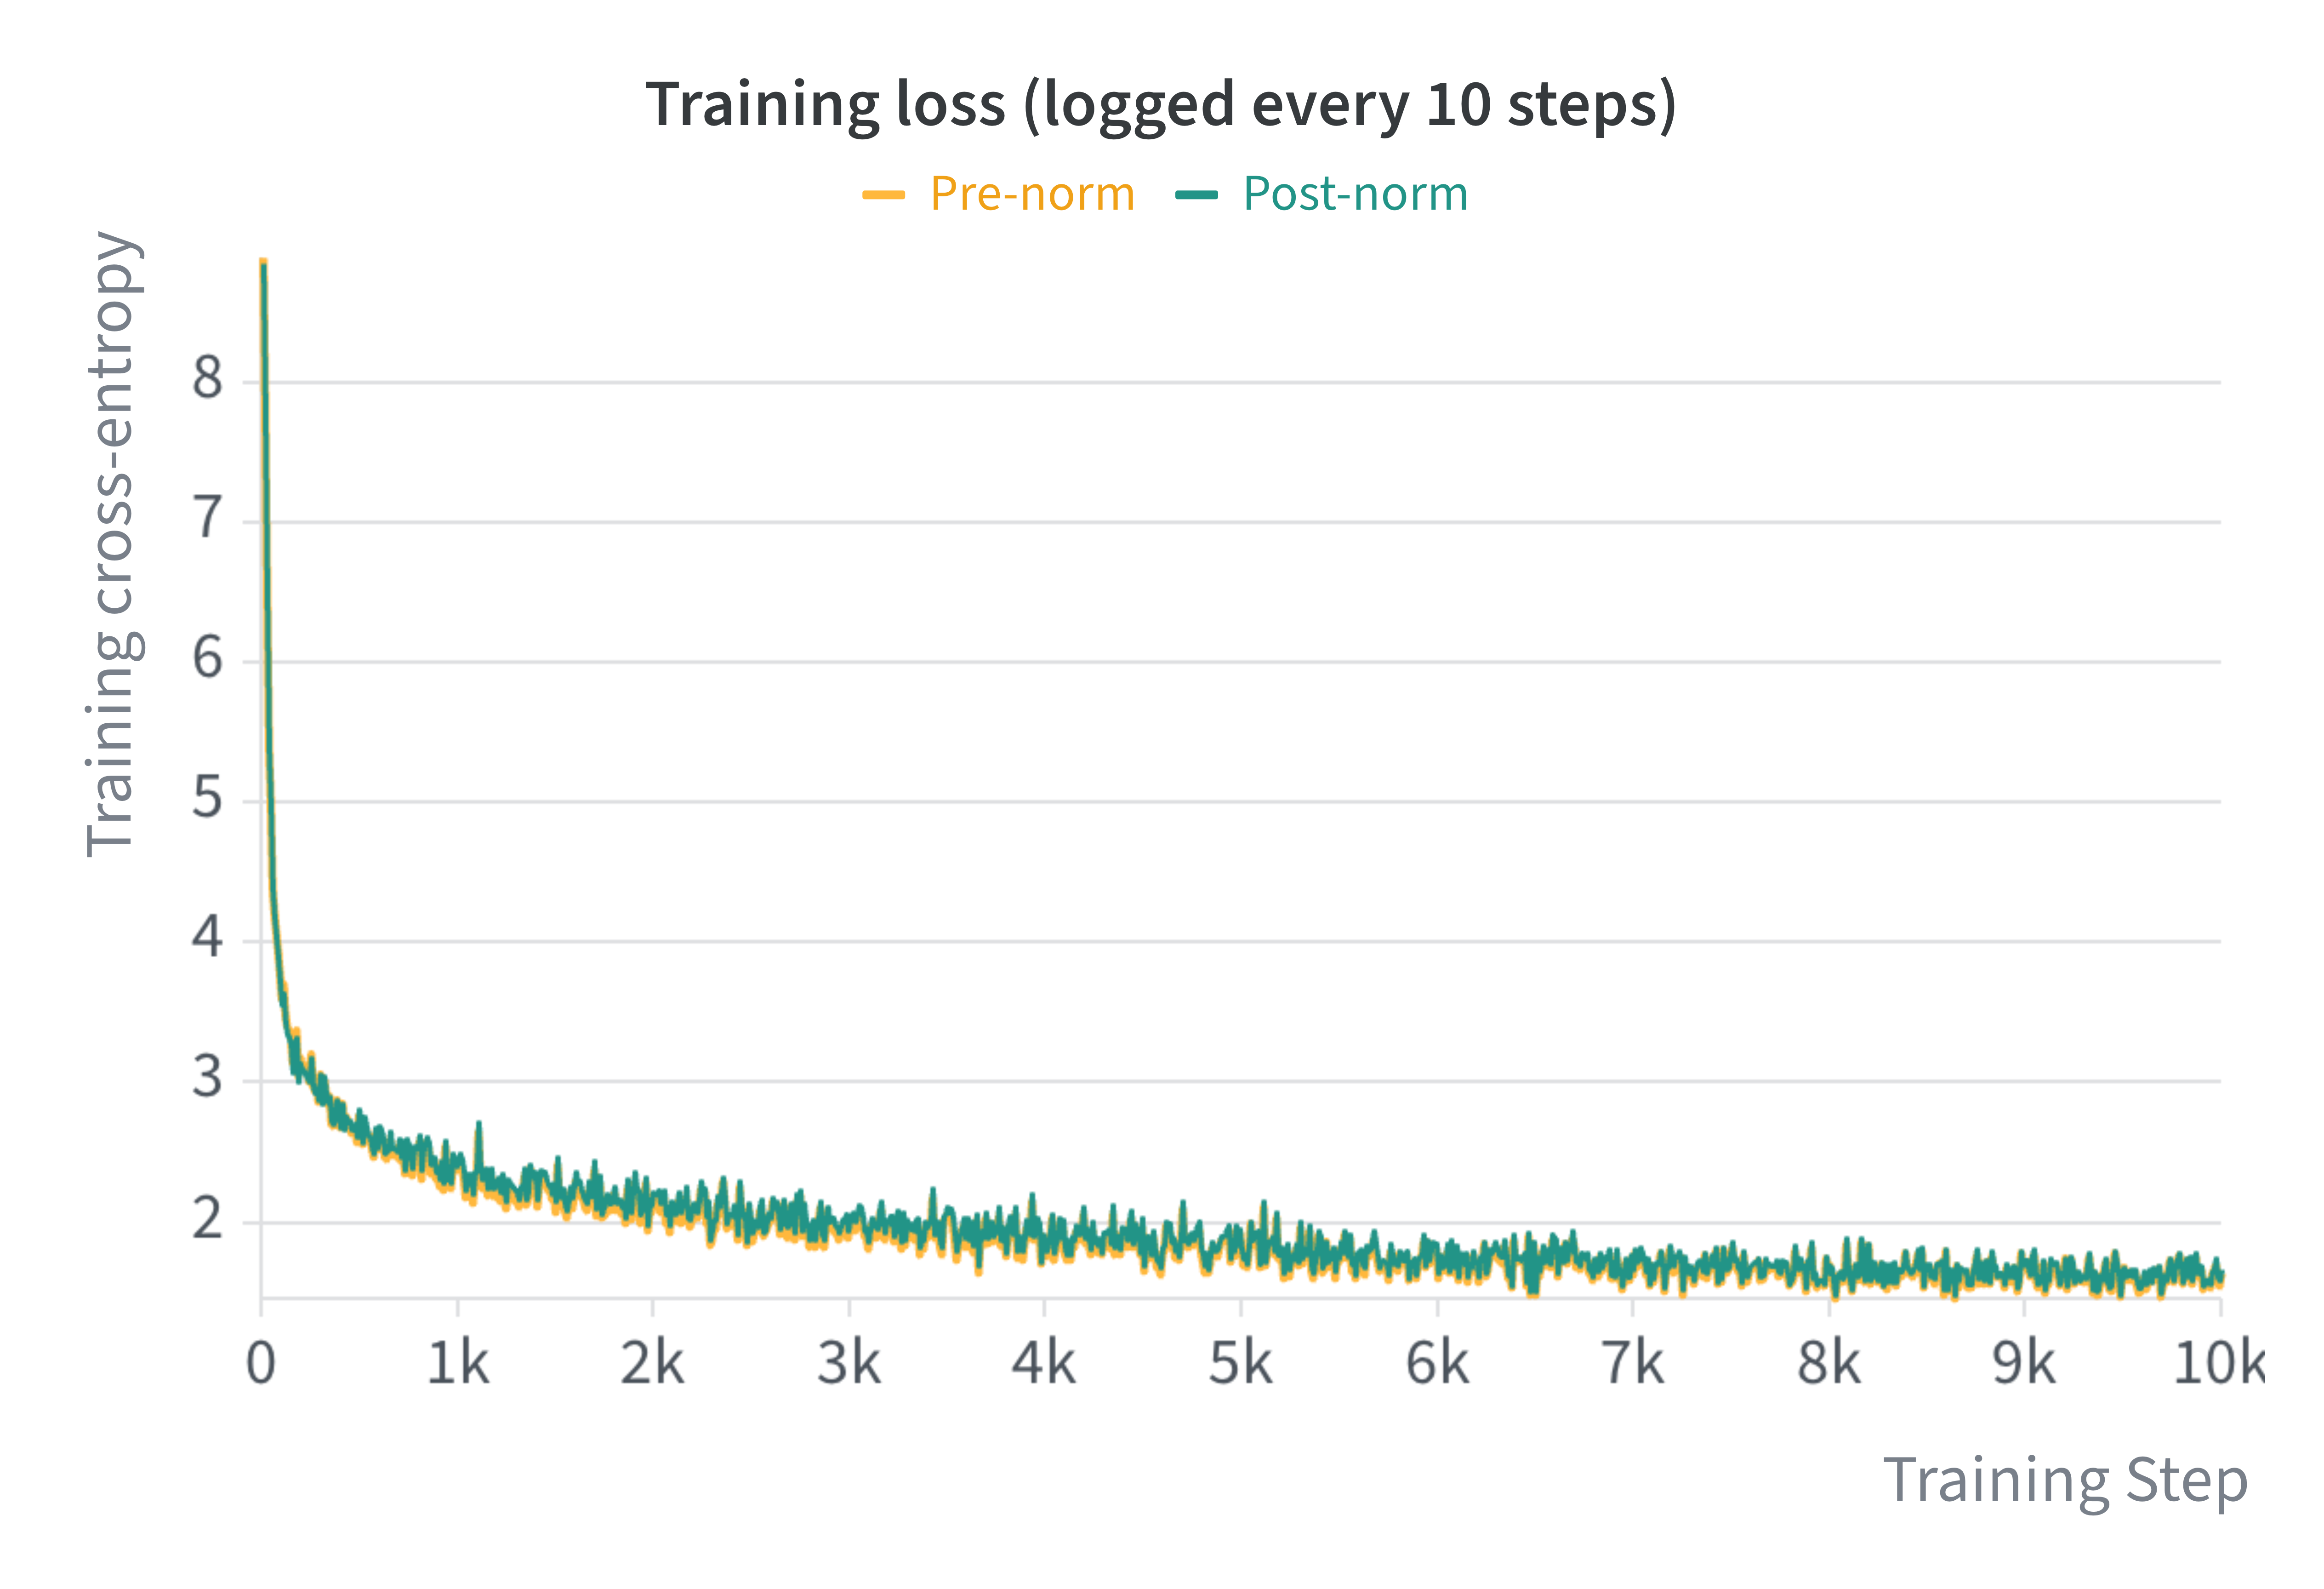
\includegraphics[width=0.49\textwidth]{figures/pre_post_norm_train.png}\hfill
    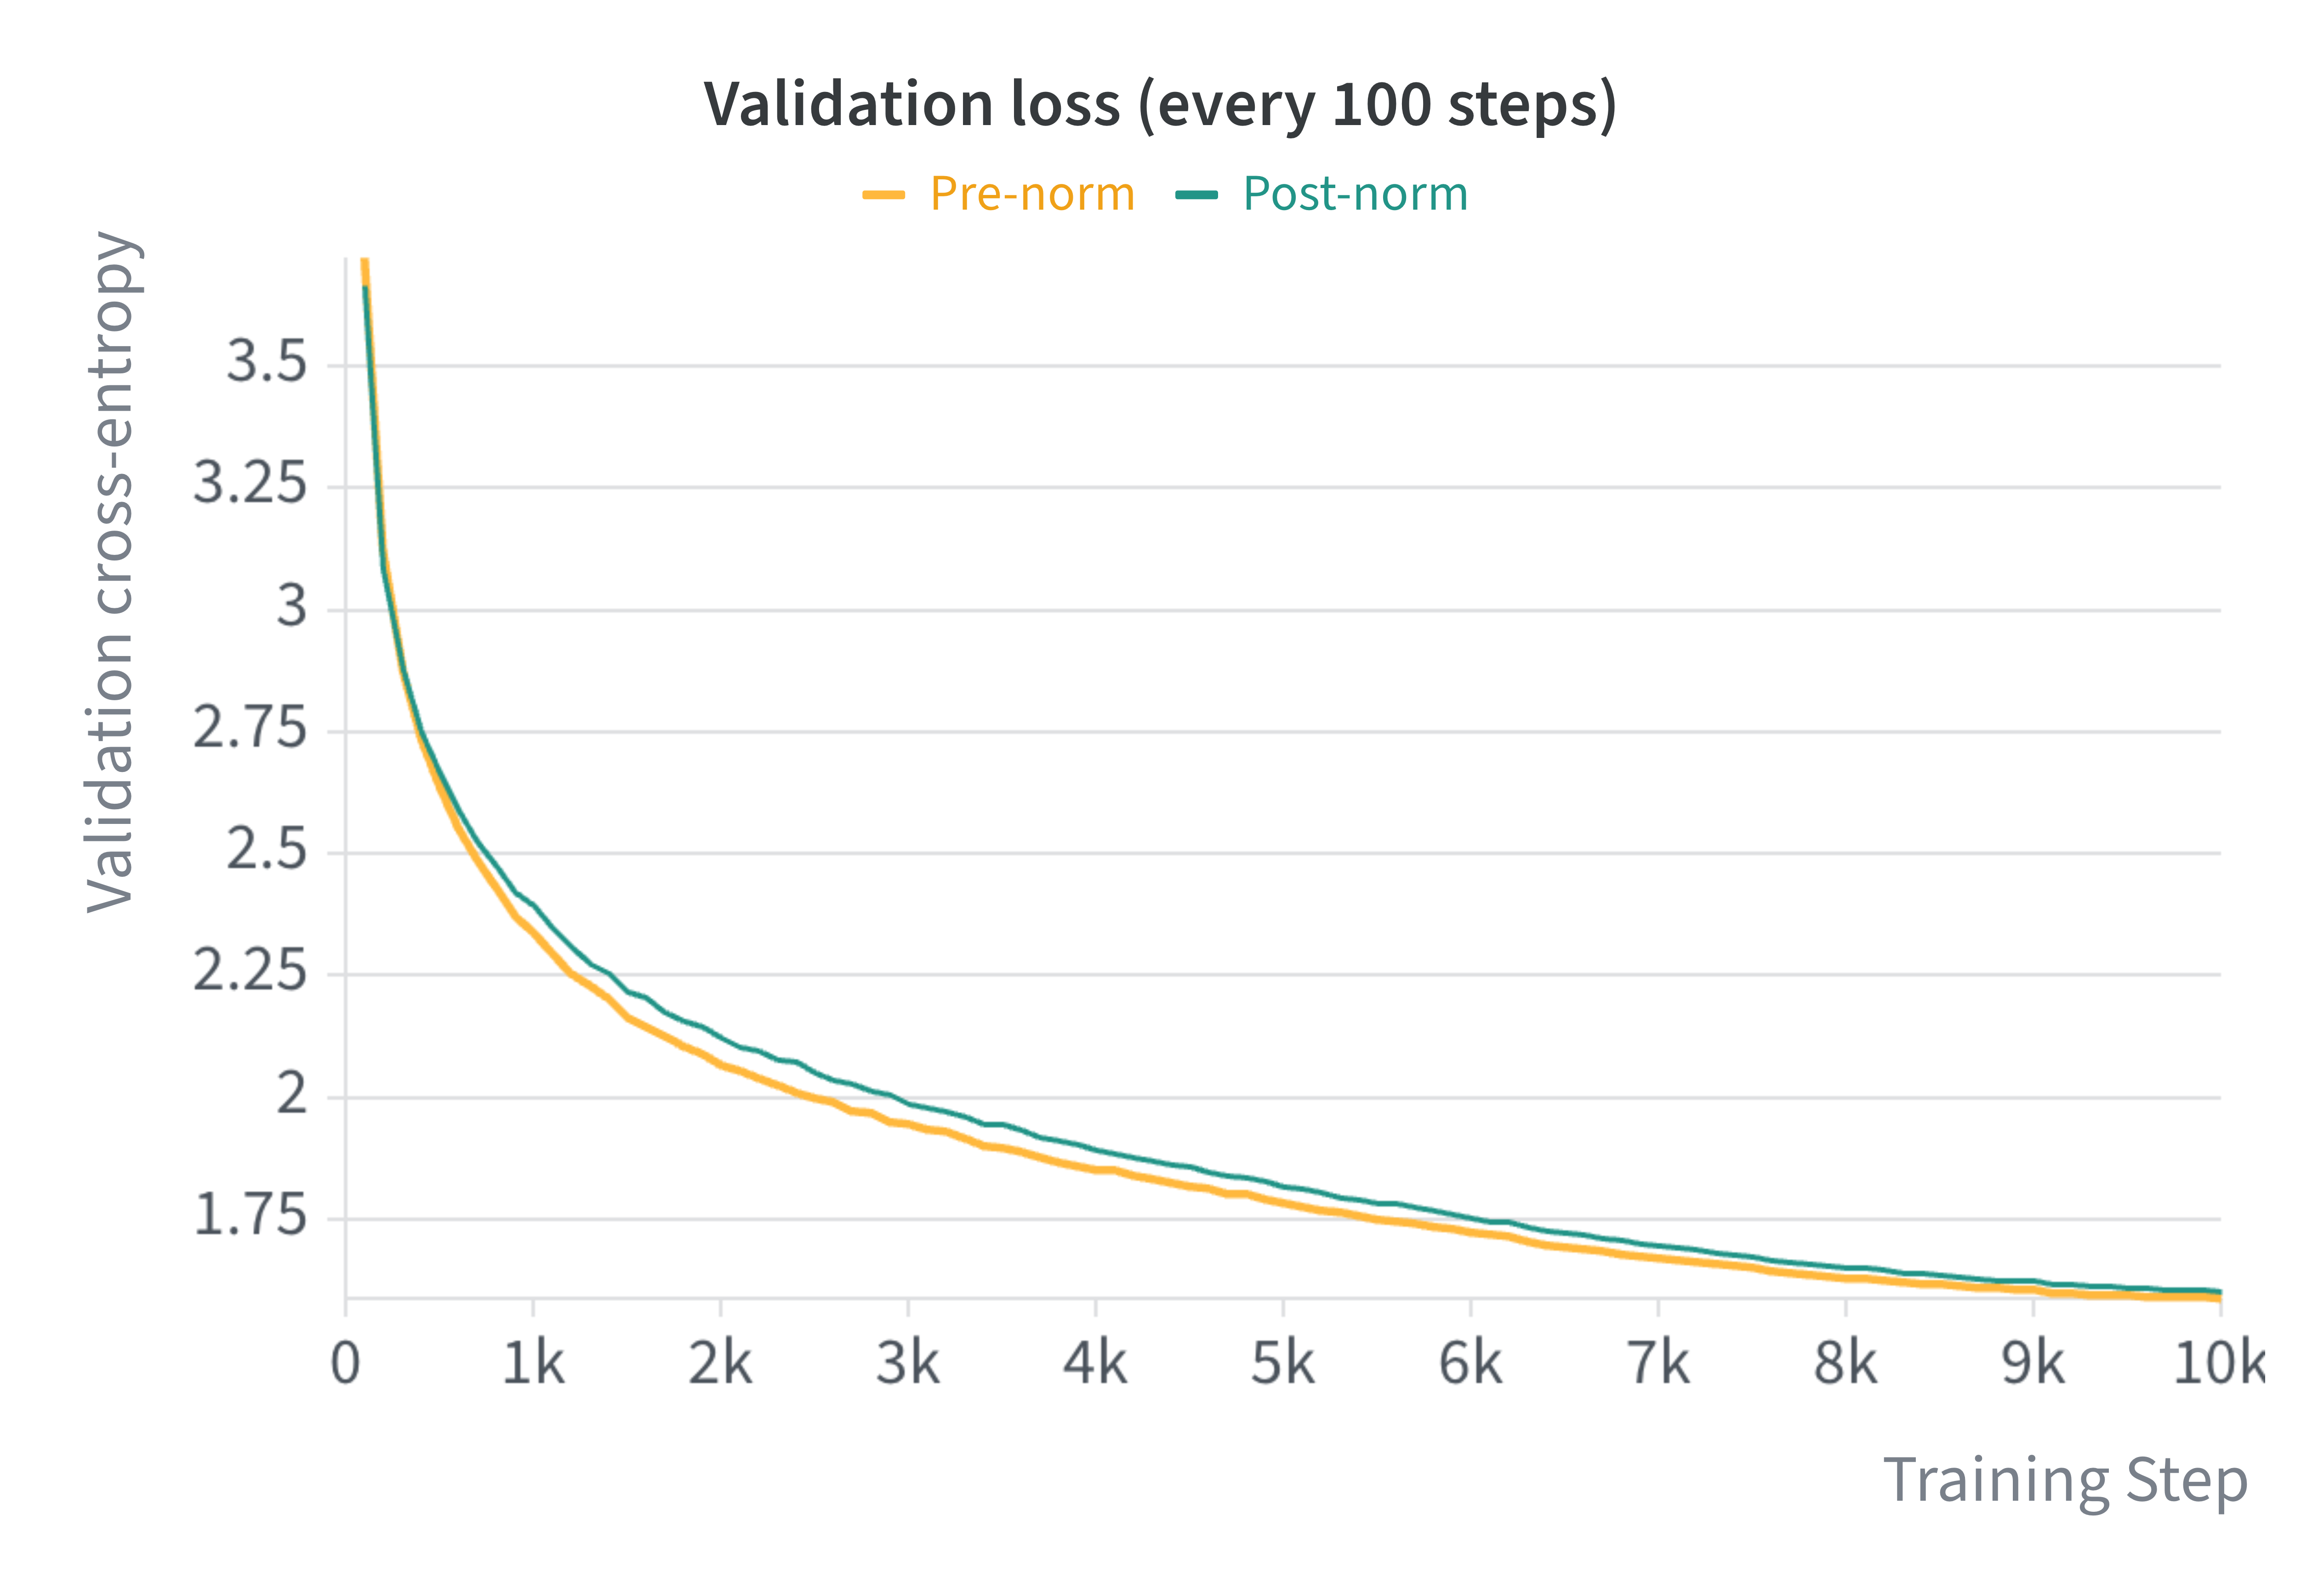
\includegraphics[width=0.49\textwidth]{figures/pre_post_norm_val.png}
    \caption{Pre-norm versus post-norm W\&B training loss (left) and validation
    loss (right), both at peak LR $10^{-3}$. Both panels cover the full run.}
    \label{fig:pre_norm_ablation}
\end{figure}

Both variants trained without comparable loss explosions. Post-norm was
slightly better at the first two evaluations, but had higher validation loss
at the remaining 98 evaluations. It ended at 1.6042 versus 1.5879 for
pre-norm, a gap of 0.0163. Pre-norm therefore performed slightly better
under this shared schedule; post-norm was still trainable in this four-layer
model. This single-seed comparison does not establish that post-norm is
inherently unstable or that the small final gap is statistically significant.

\problem{no\_pos\_emb}{Implement NoPE}{1}

I removed RoPE from every attention layer while retaining the causal mask.
This changes no trainable parameter counts; all other common settings,
including the LR schedule, were fixed.

\begin{figure}[H]
    \centering
    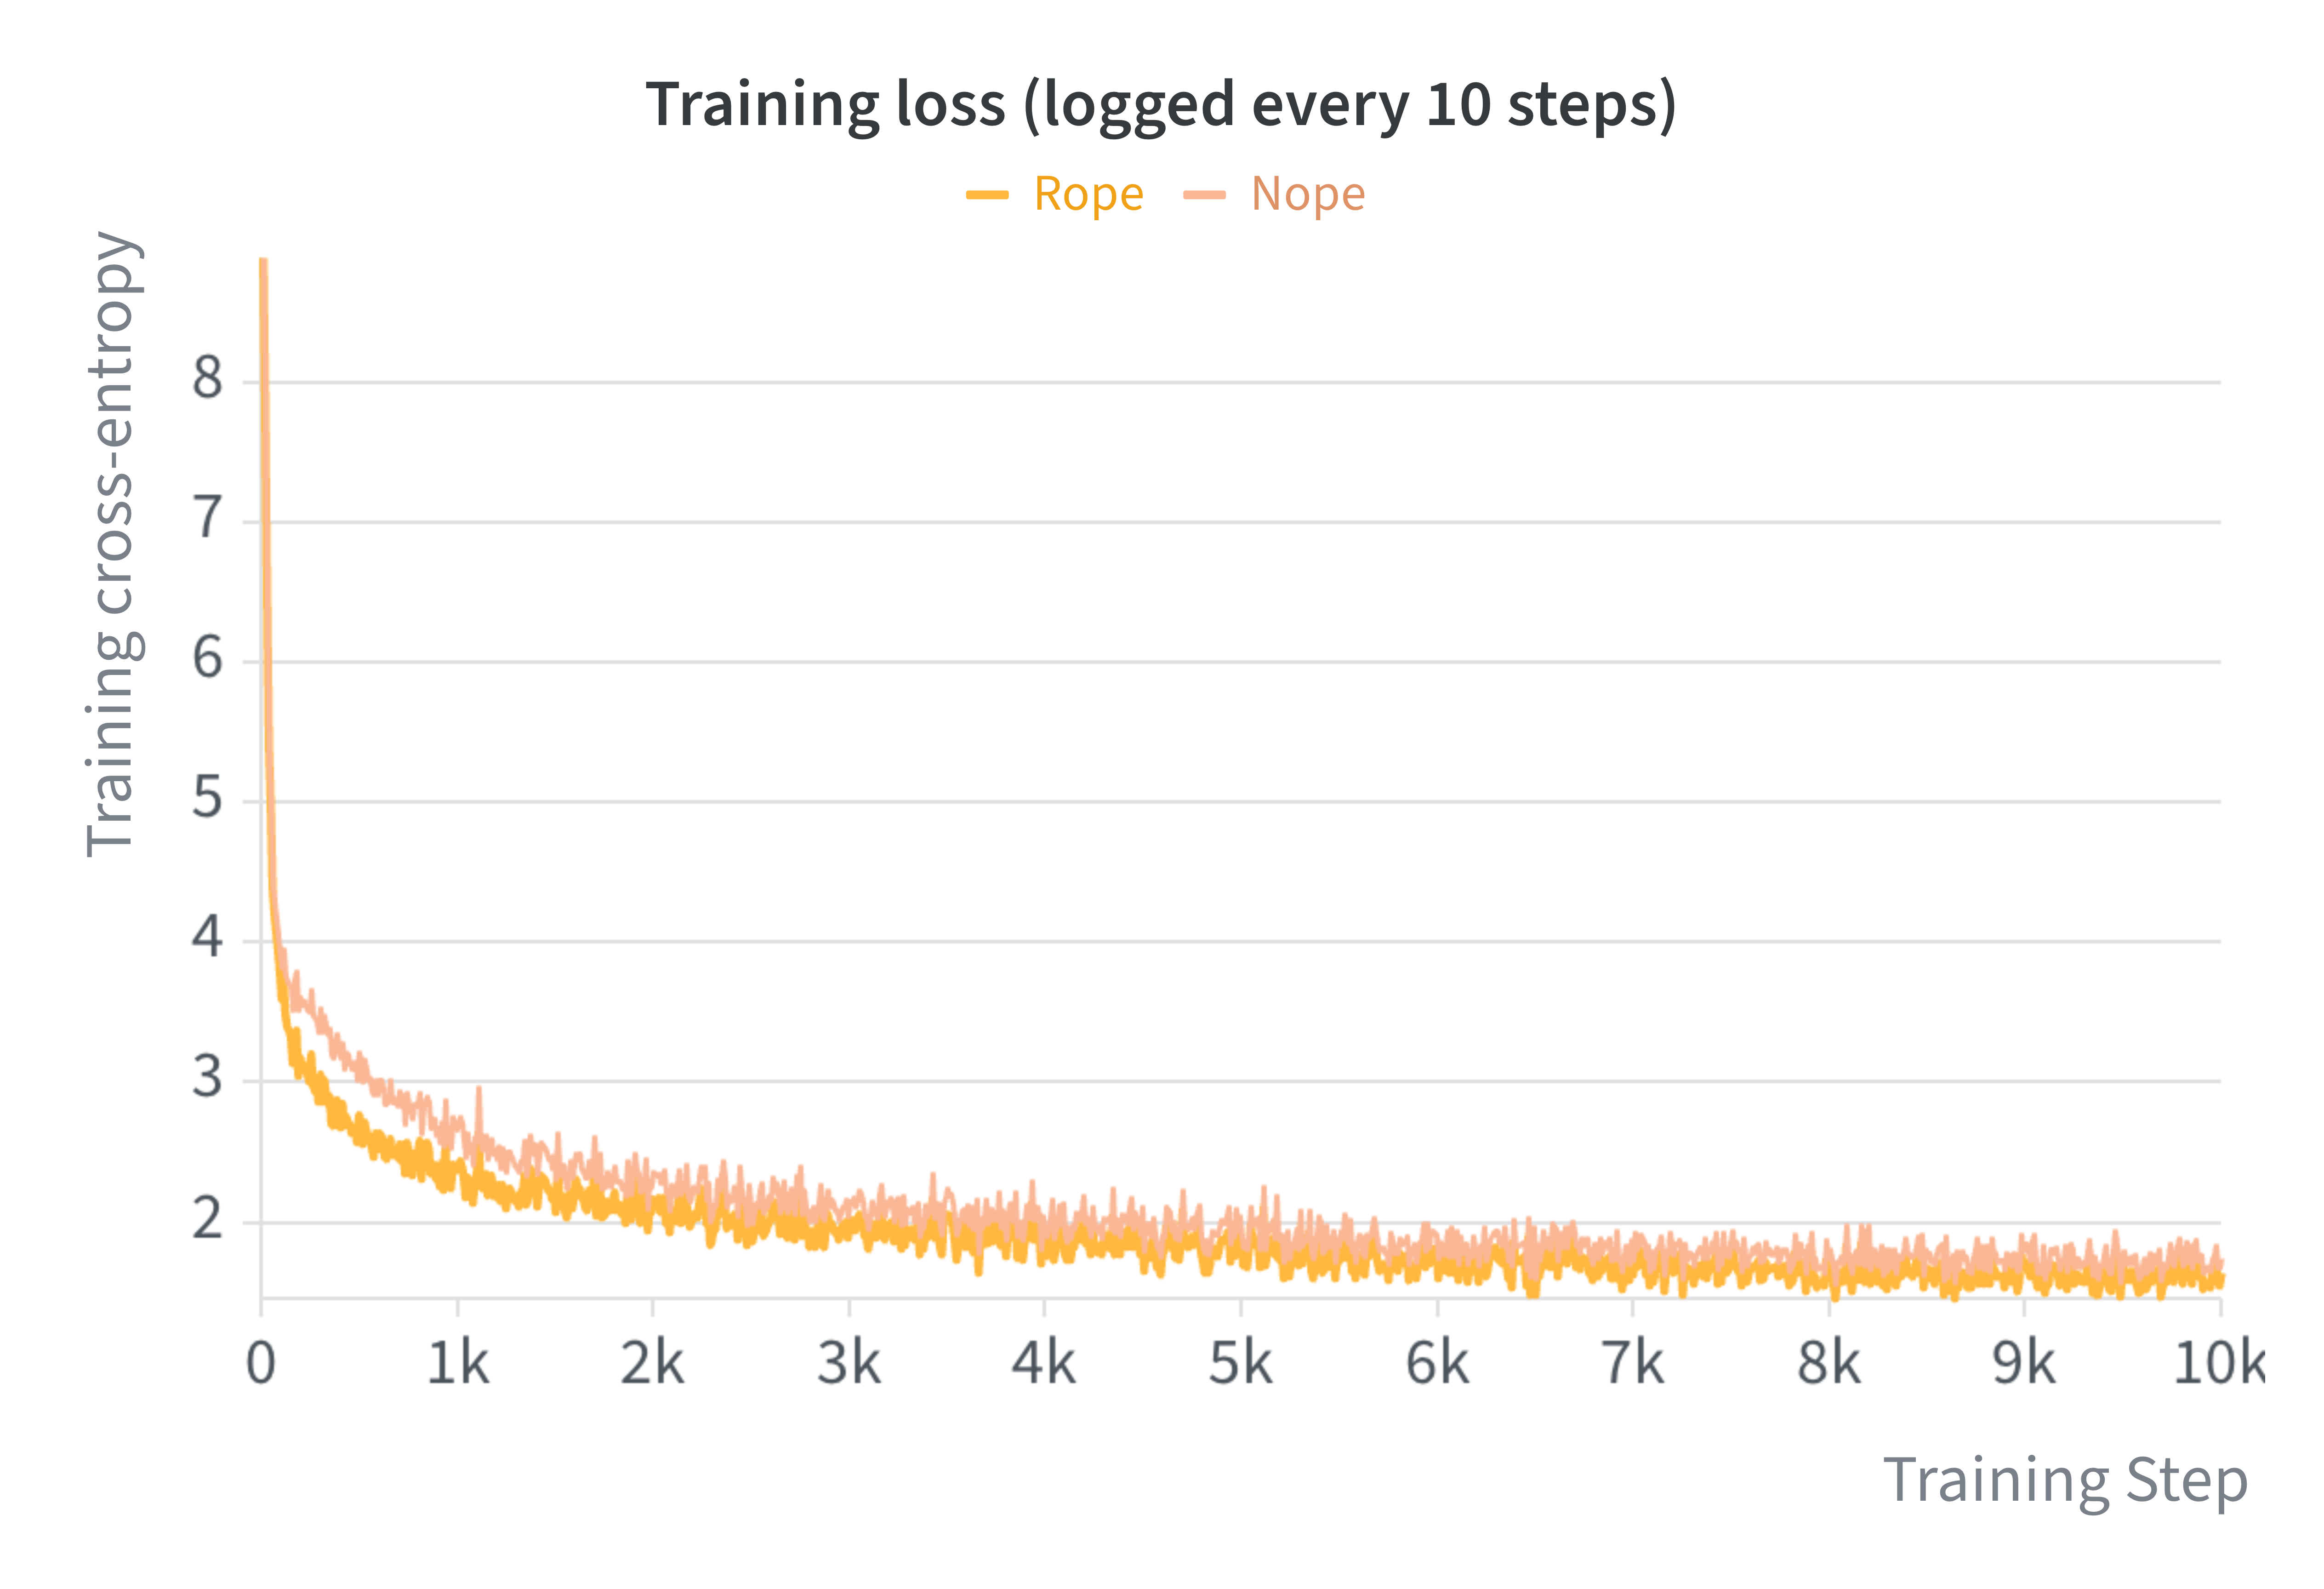
\includegraphics[width=0.49\textwidth]{figures/rope_nope_train.png}\hfill
    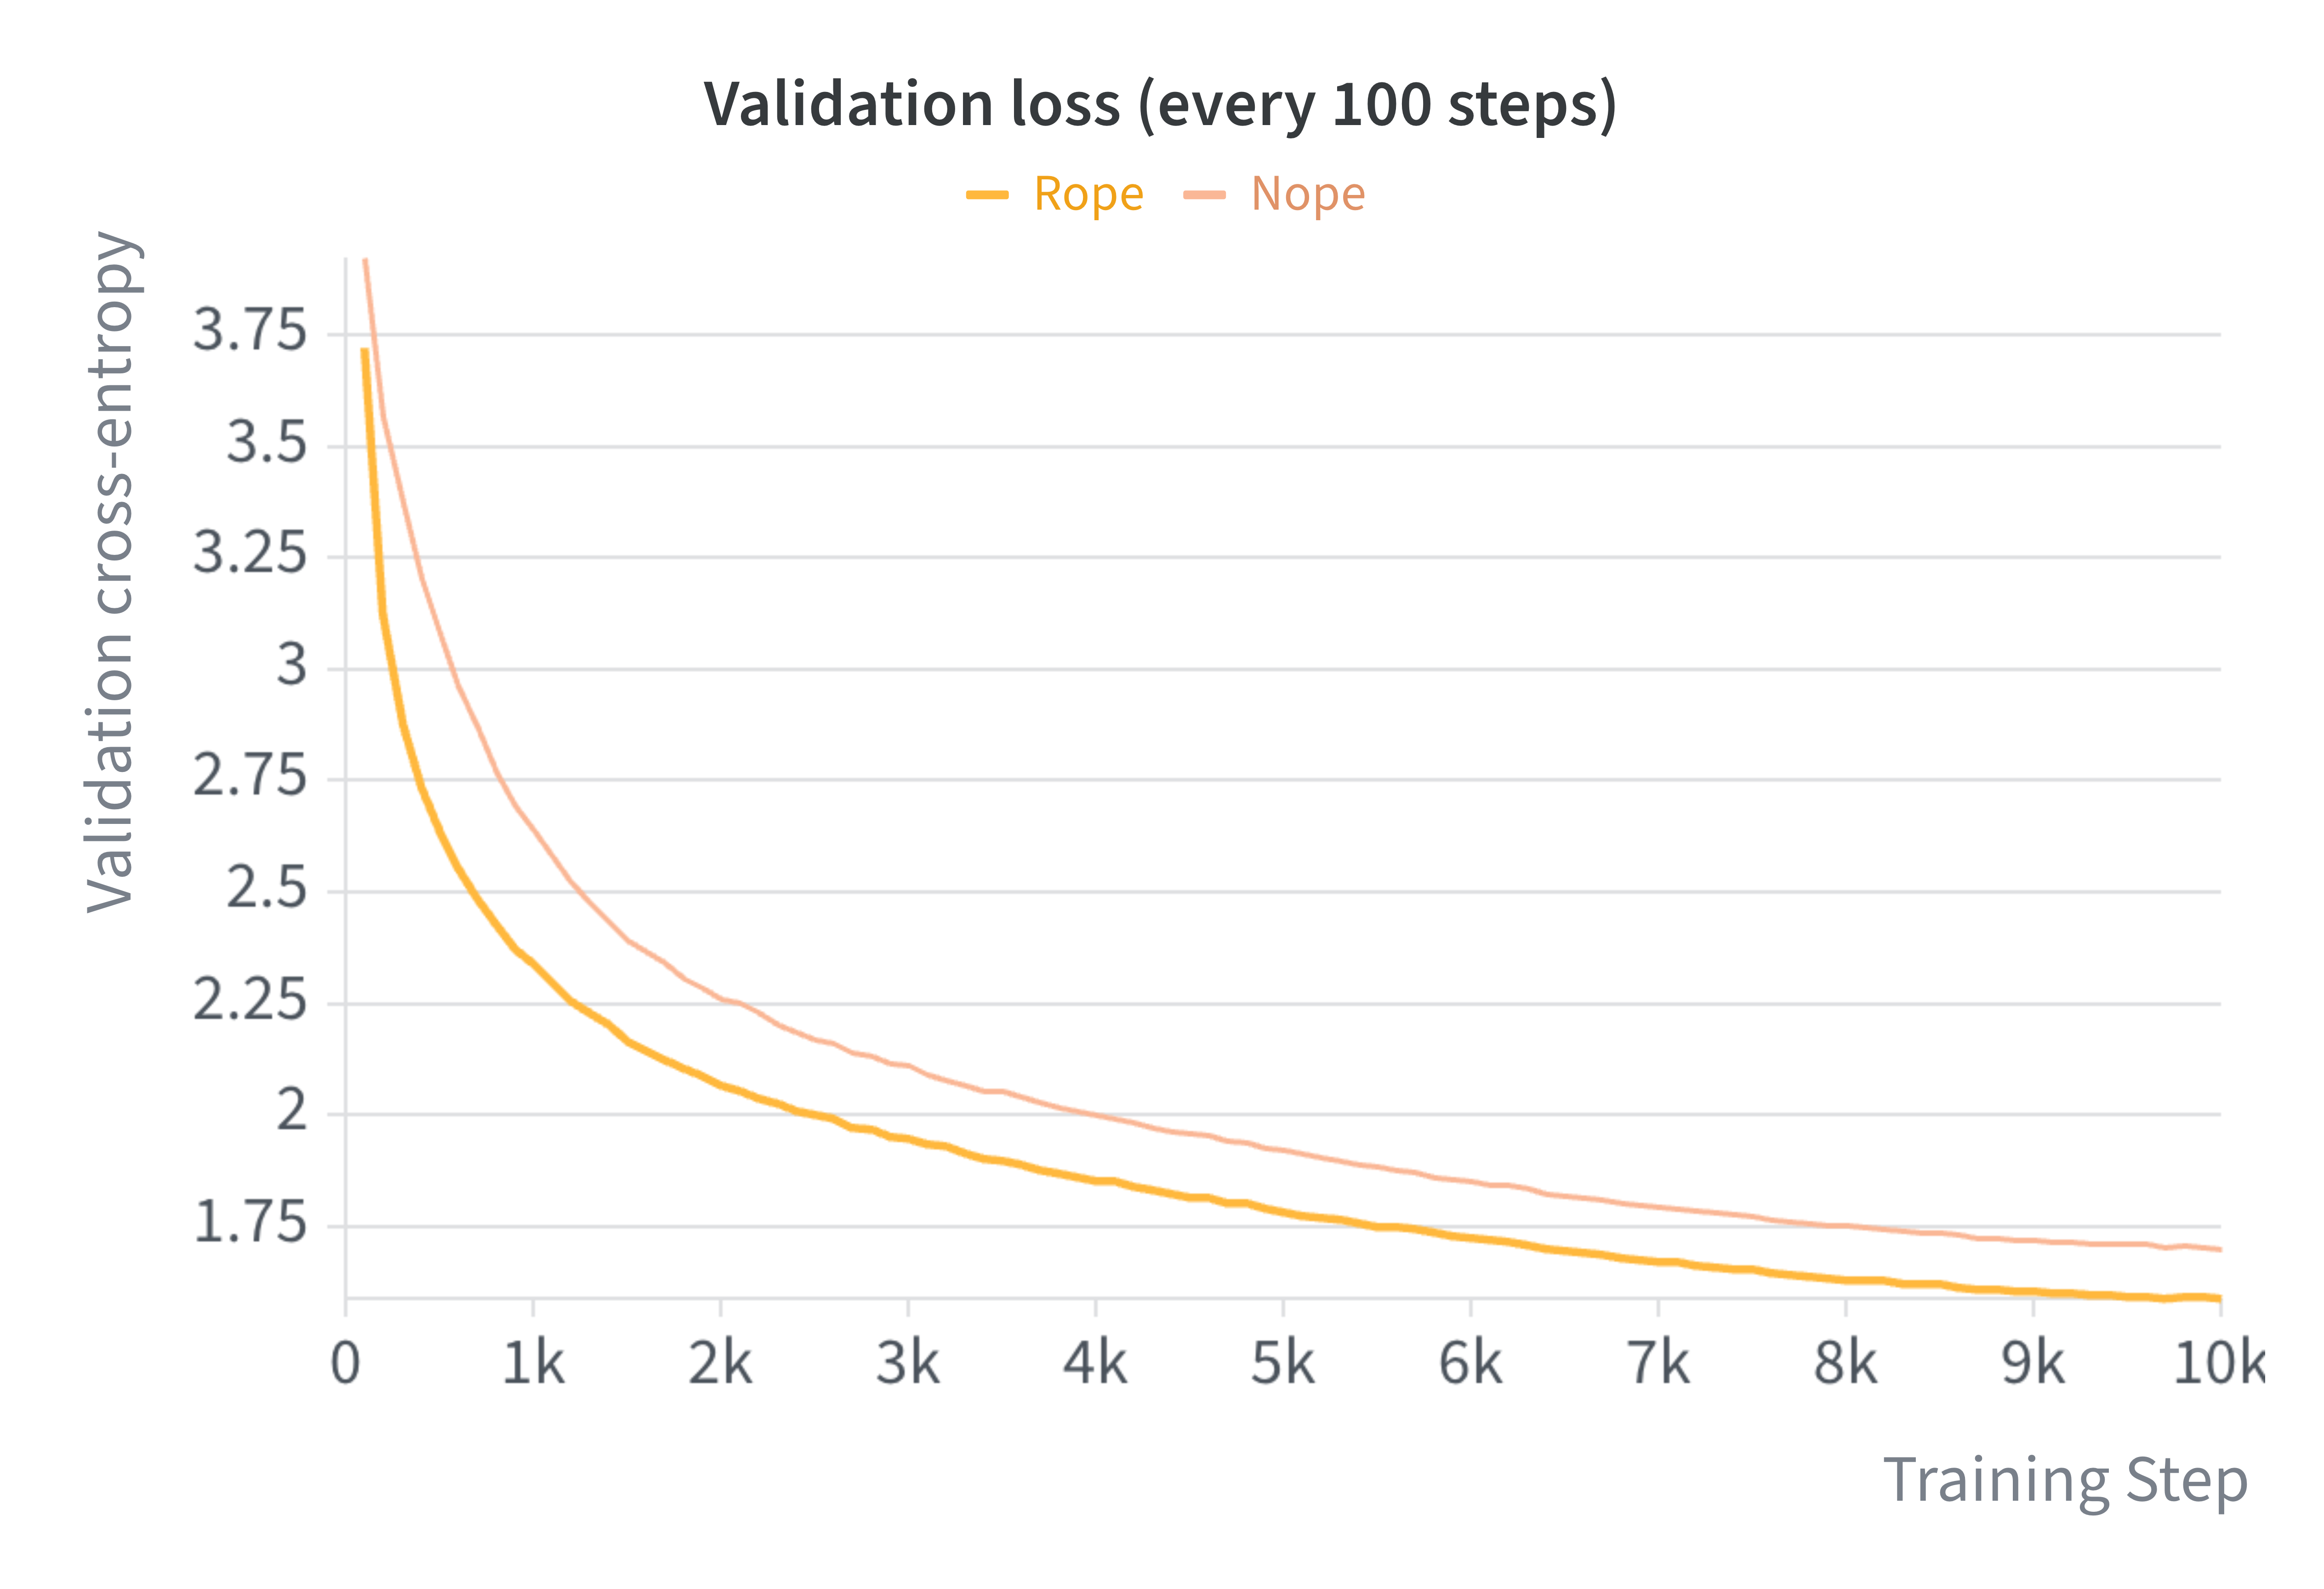
\includegraphics[width=0.49\textwidth]{figures/rope_nope_val.png}
    \caption{RoPE versus NoPE W\&B training loss (left) and validation loss
    (right). Both panels cover the full run; causal masking is present in
    both models.}
    \label{fig:nope_vs_rope}
\end{figure}

NoPE learned stably but had higher loss at all 100 matched evaluations.
It reached 1.7010 versus 1.5879 for RoPE, a gap of 0.1131, the largest
observed gap among these four architecture variants. Removing explicit
position information therefore hurt performance under this training budget.
The model still learned without RoPE; the result does not imply that a
causally masked Transformer cannot represent positional information.
These measurements concern context length 256 and do not test length
extrapolation or establish an optimal LR for NoPE.

\problem{swiglu\_ablation}{SwiGLU vs.\ SiLU}{1}

I replaced the gated feed-forward network with
$\operatorname{FFN}_{\mathrm{SiLU}}(x)=W_2\operatorname{SiLU}(W_1x)$.
The SiLU hidden width was $4d_{\mathrm{model}}=2048$, compared with 1344
for SwiGLU. This approximately matches the feed-forward parameter budget:
$2\times512\times2048=2{,}097{,}152$ versus
$3\times512\times1344=2{,}064{,}384$ weights per block.
Total model sizes were 22,827,520 and 22,696,448 parameters, respectively,
a difference of about 0.58\%. All other common settings were fixed.

\begin{figure}[H]
    \centering
    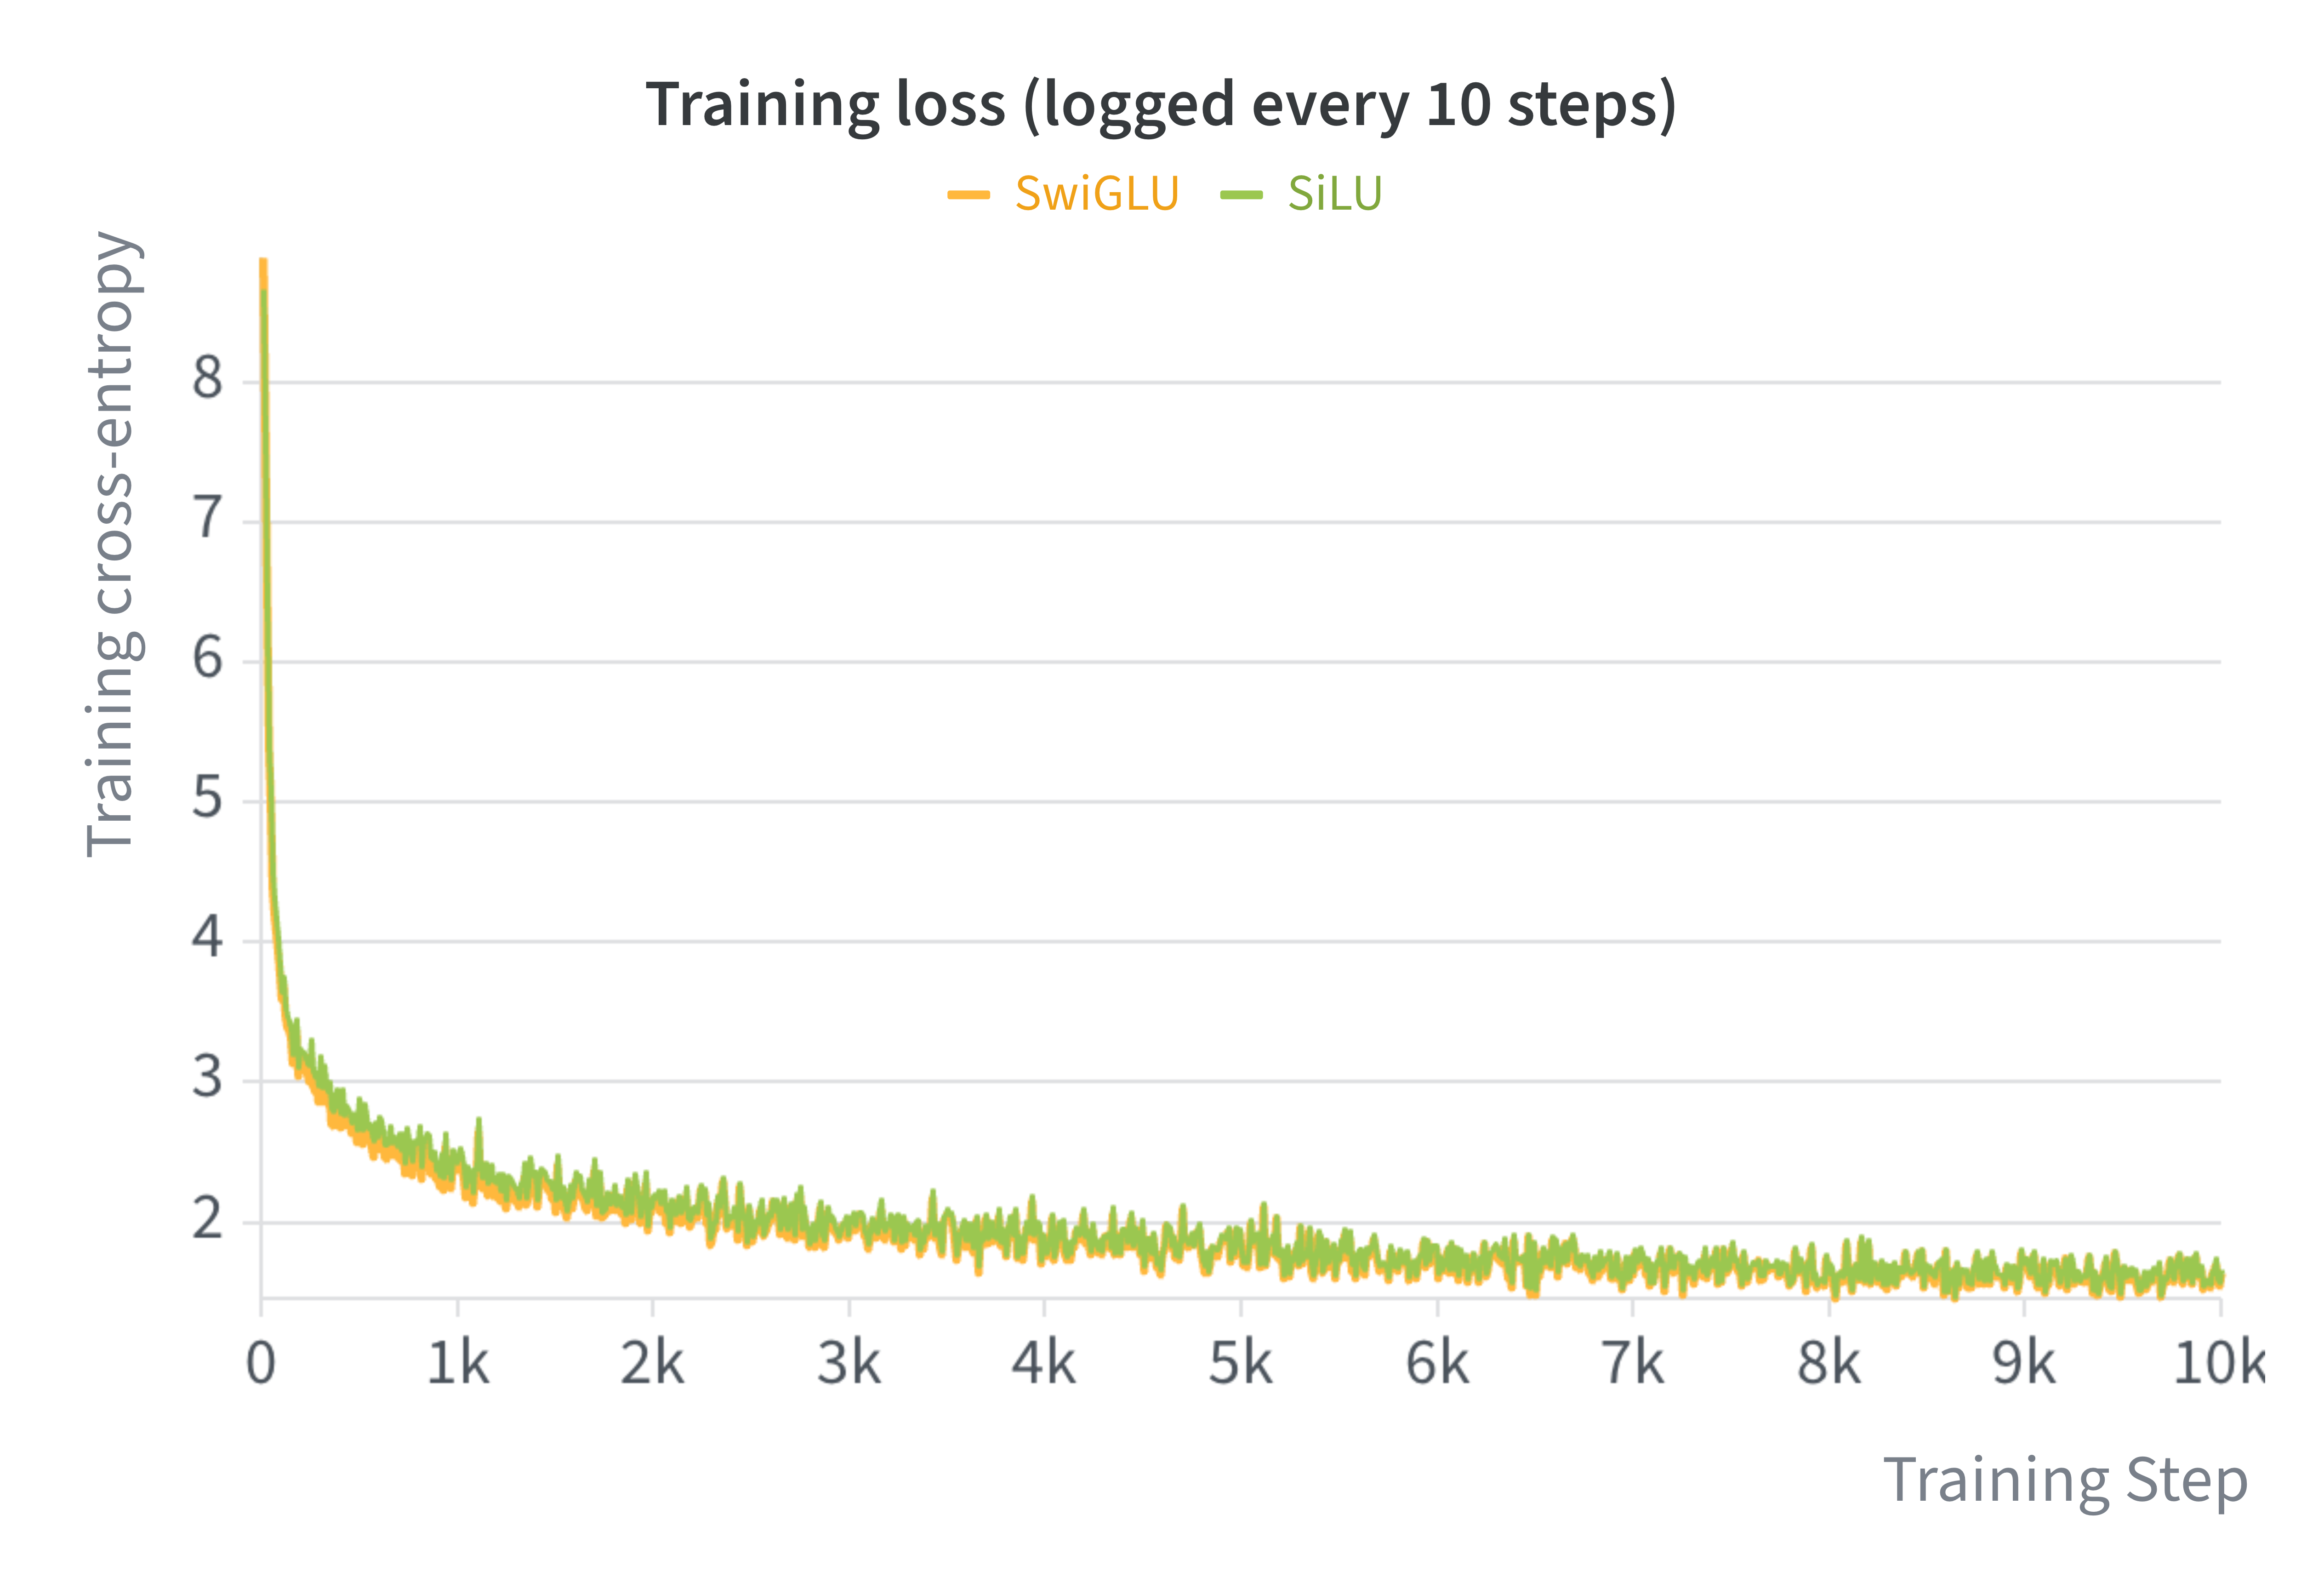
\includegraphics[width=0.49\textwidth]{figures/swiglu_silu_train.png}\hfill
    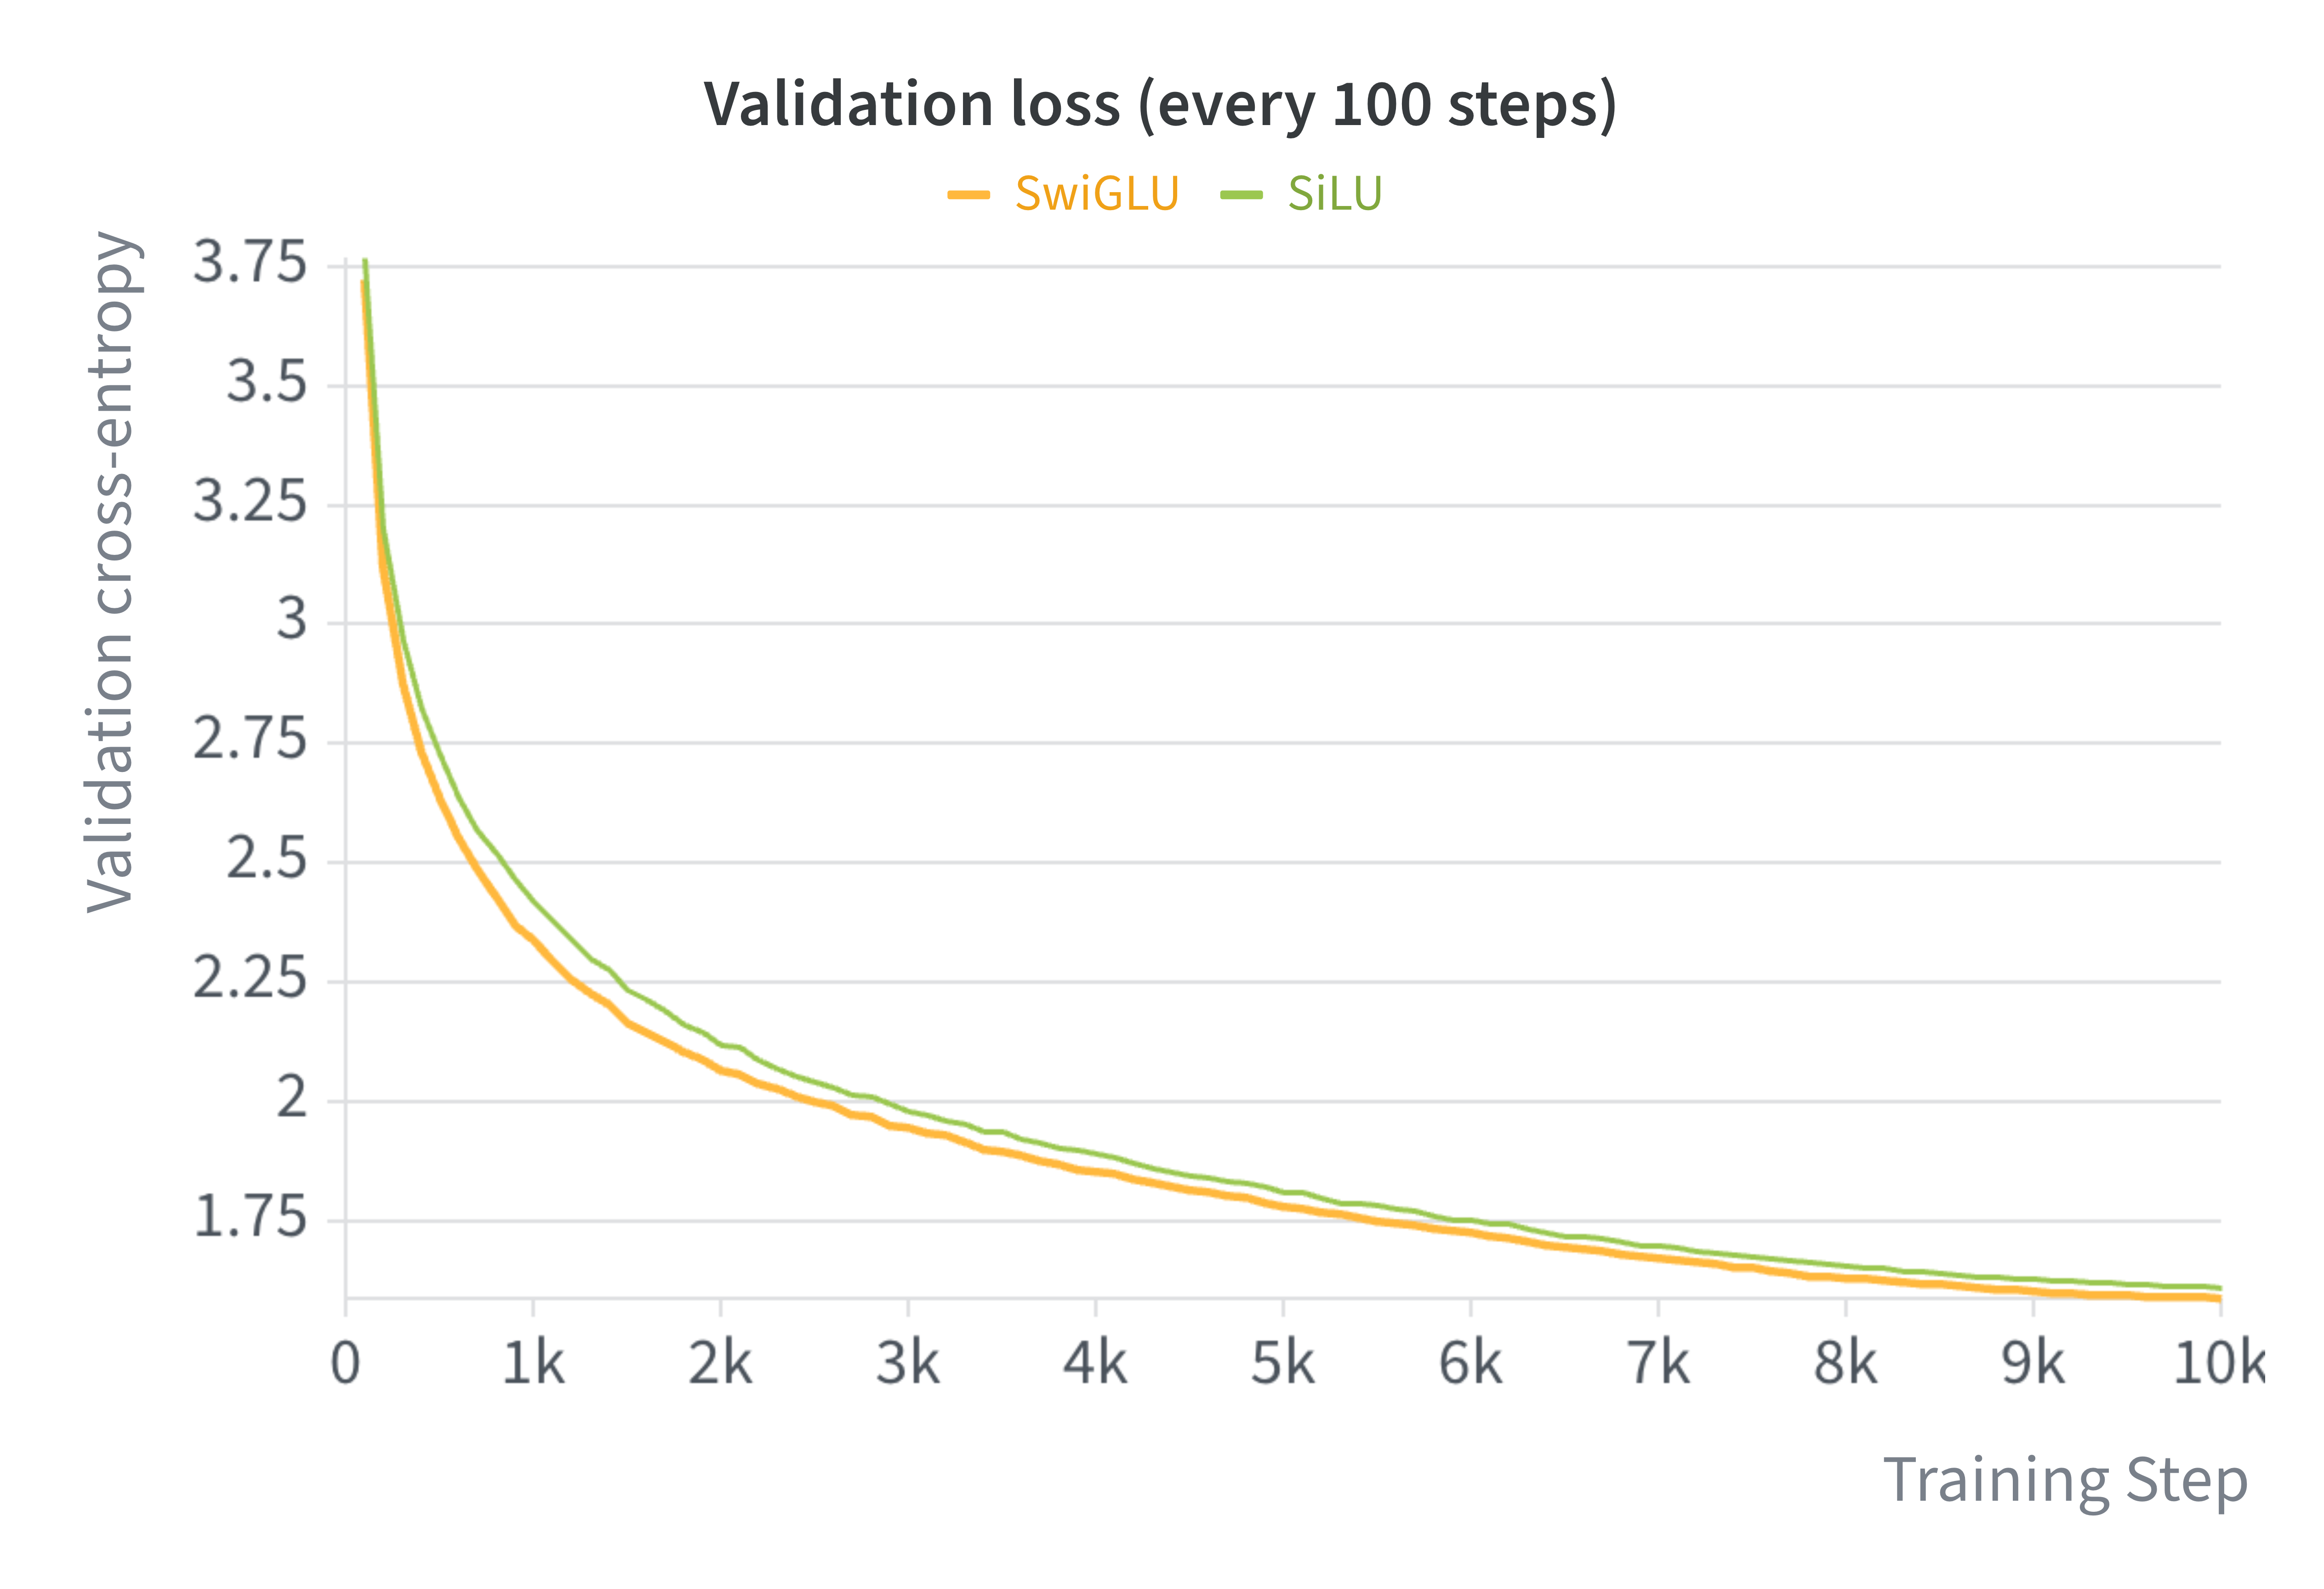
\includegraphics[width=0.49\textwidth]{figures/swiglu_silu_val.png}
    \caption{SwiGLU versus SiLU W\&B training loss (left) and validation loss
    (right), with approximately matched parameter counts. Orange denotes
    SwiGLU and green denotes SiLU in both panels.}
    \label{fig:swiglu_vs_silu}
\end{figure}

Both variants trained stably. SiLU had higher loss at every matched evaluation
and ended at 1.6106, compared with 1.5879 for SwiGLU, a gap of 0.0227.
The gated network performed modestly better in this run despite having
slightly fewer parameters, consistent with a benefit from gating at this
budget. Because only one seed and a shared LR schedule were tested, this
is an observed advantage for the chosen configuration, not a claim of
statistical significance or universal superiority.

\FloatBarrier
\Needspace{35\baselineskip}
\problem{main\_experiment}{Experiment on OWT}{2}
\label{prob:owt}

OWT used the standard TinyStories backbone, batch 16, context 256, and
80,000 updates (327.68M tokens), retaining its 32k tokenizer. Final loss
was 3.8596, also the lowest sampled value. Compared with low-resource
OWT's 4.4561, the longer recipe improved by 0.5965 nats per token.
Settings are in Appendix~\ref{app:standard_protocol}.

\begin{table}[htbp]
    \centering\small
    \begin{tabular}{@{}lrrrr@{}}
        \toprule
        Dataset & Updates & Final val loss & Best sampled loss & Time (min) \\
        \midrule
        TinyStories & 80,000 & 1.3245 & 1.3240 at 79,200 & 66.85 \\
        OWT & 80,000 & 3.8596 & 3.8596 at 80,000 & 79.45 \\
        \bottomrule
    \end{tabular}
    \caption{Standard-budget results from the saved logs. Times are the last
    logged training elapsed times, including intervening evaluation/saving but
    excluding startup and final evaluation/checkpoint overhead.}
    \label{tab:standard_results}
\end{table}

\begin{figure}[htbp]
    \centering
    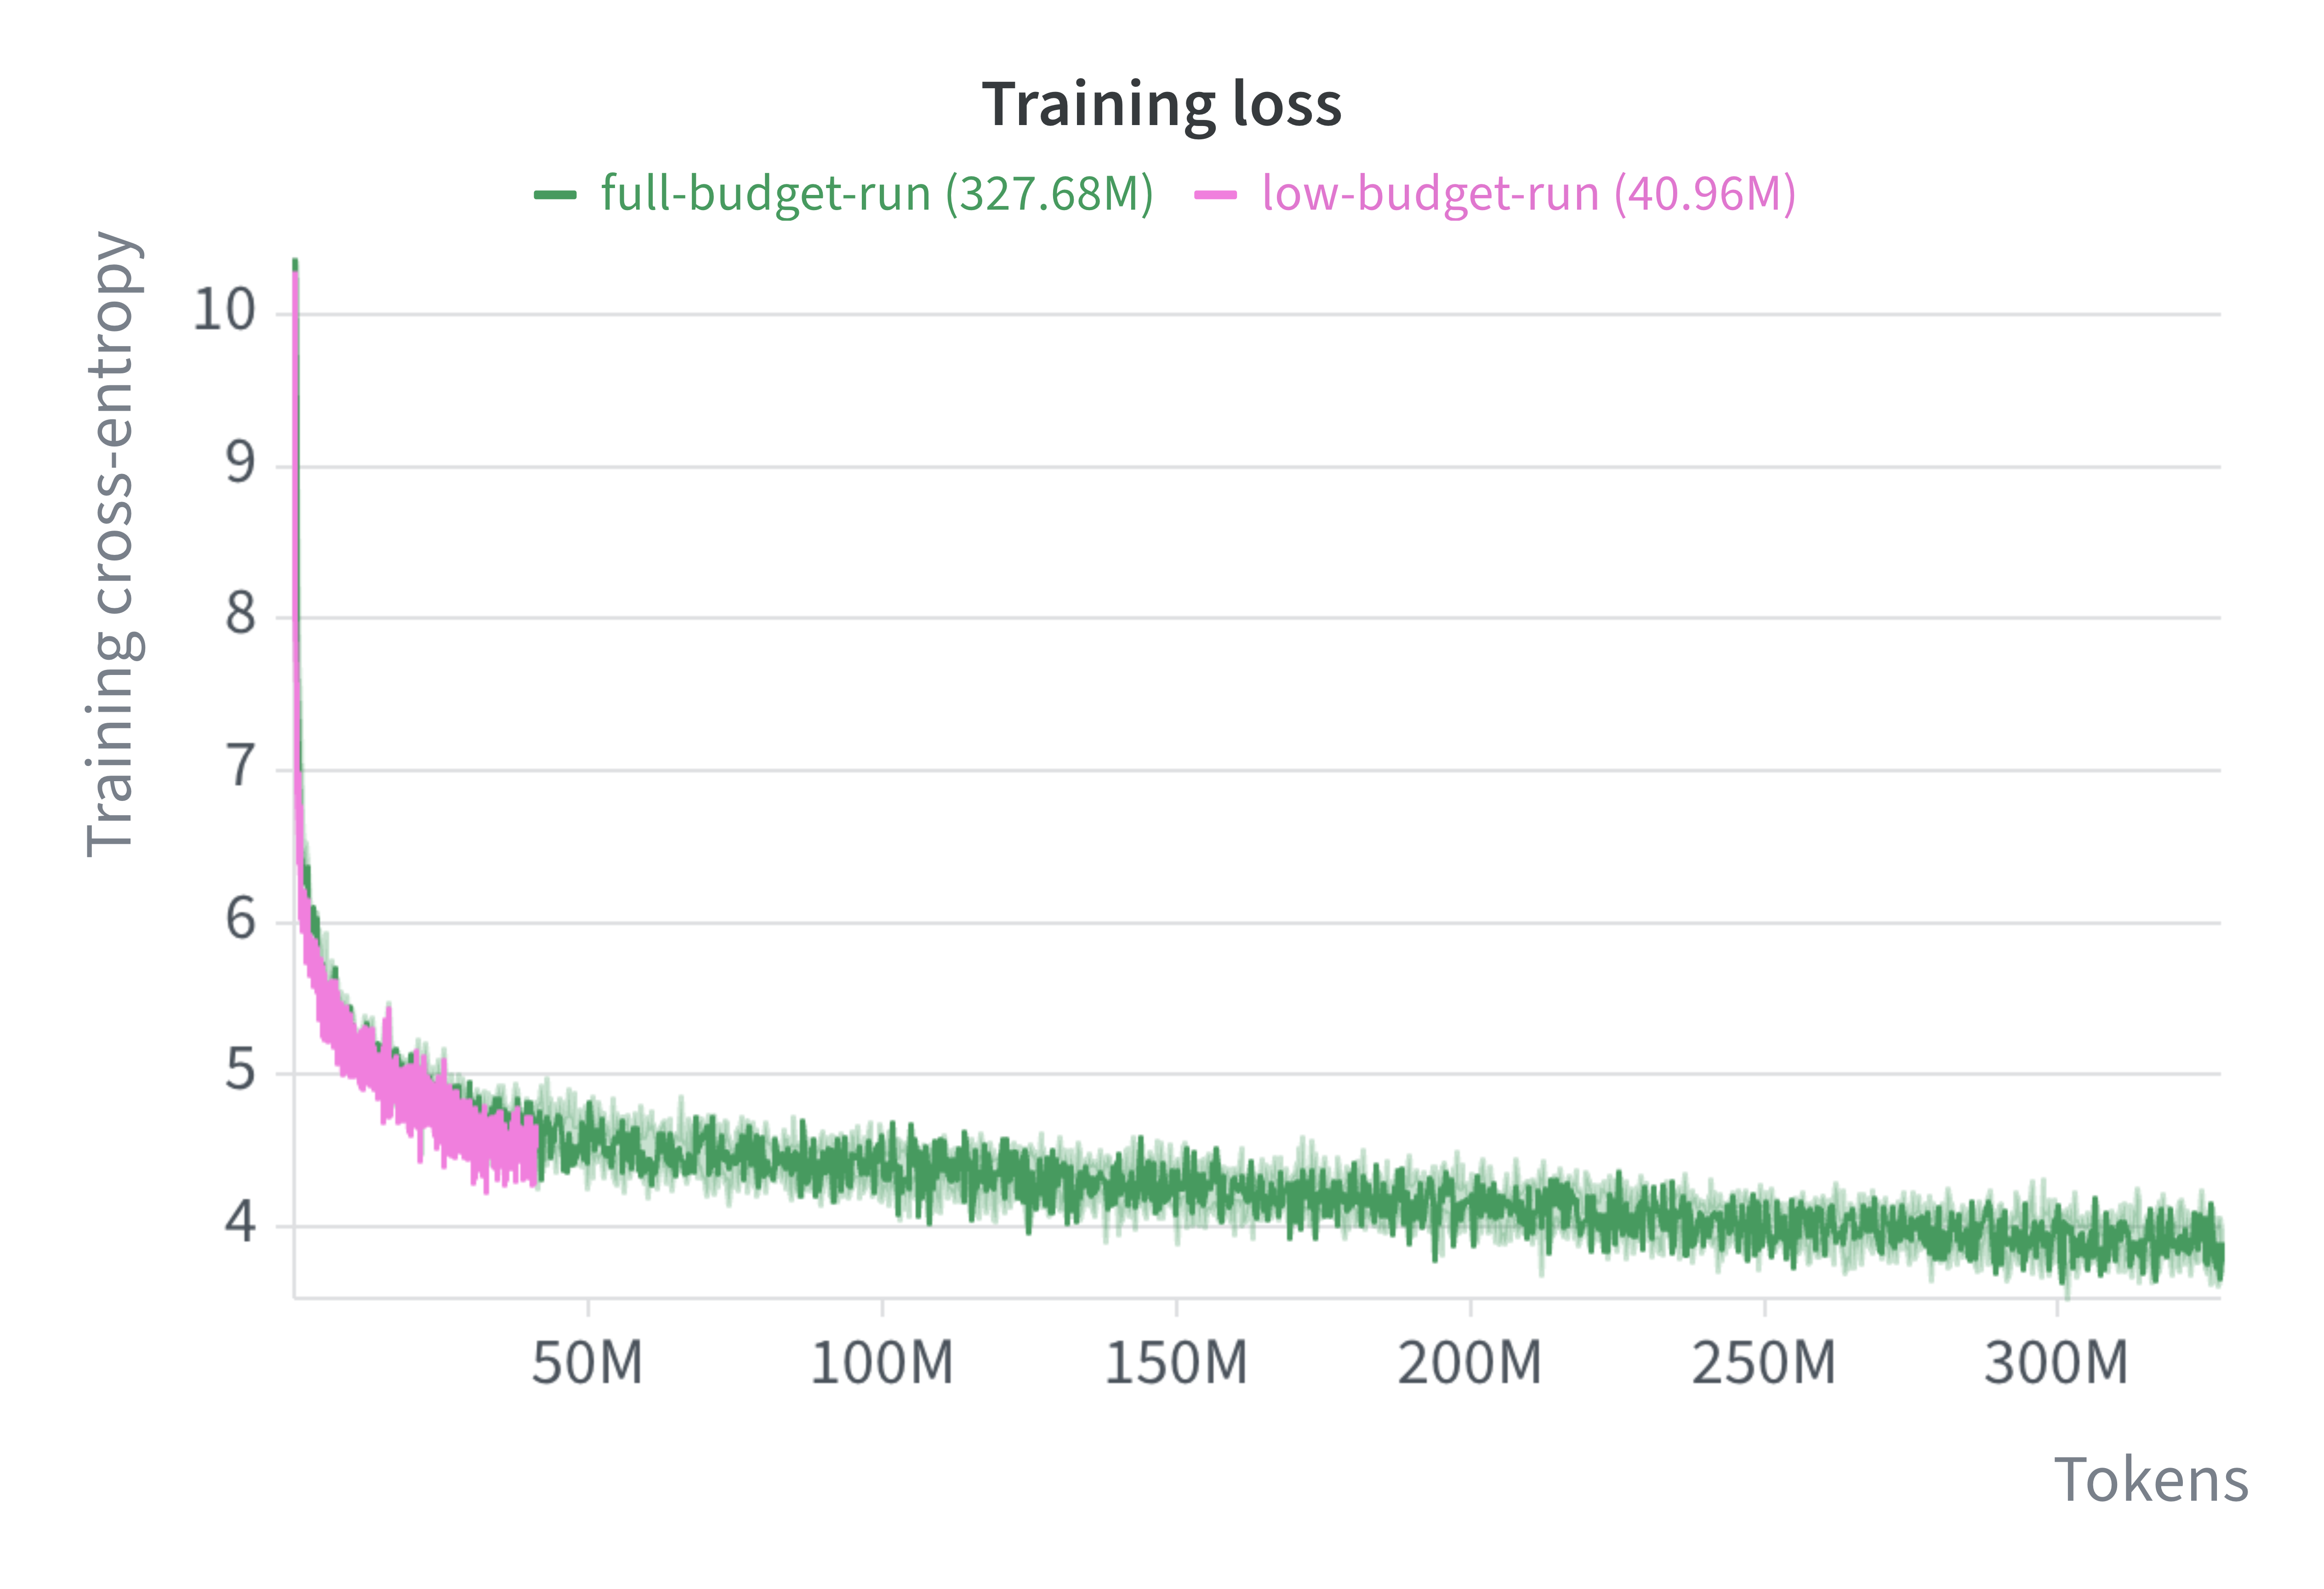
\includegraphics[width=0.49\textwidth]{figures/owt_full_train.png}\hfill
    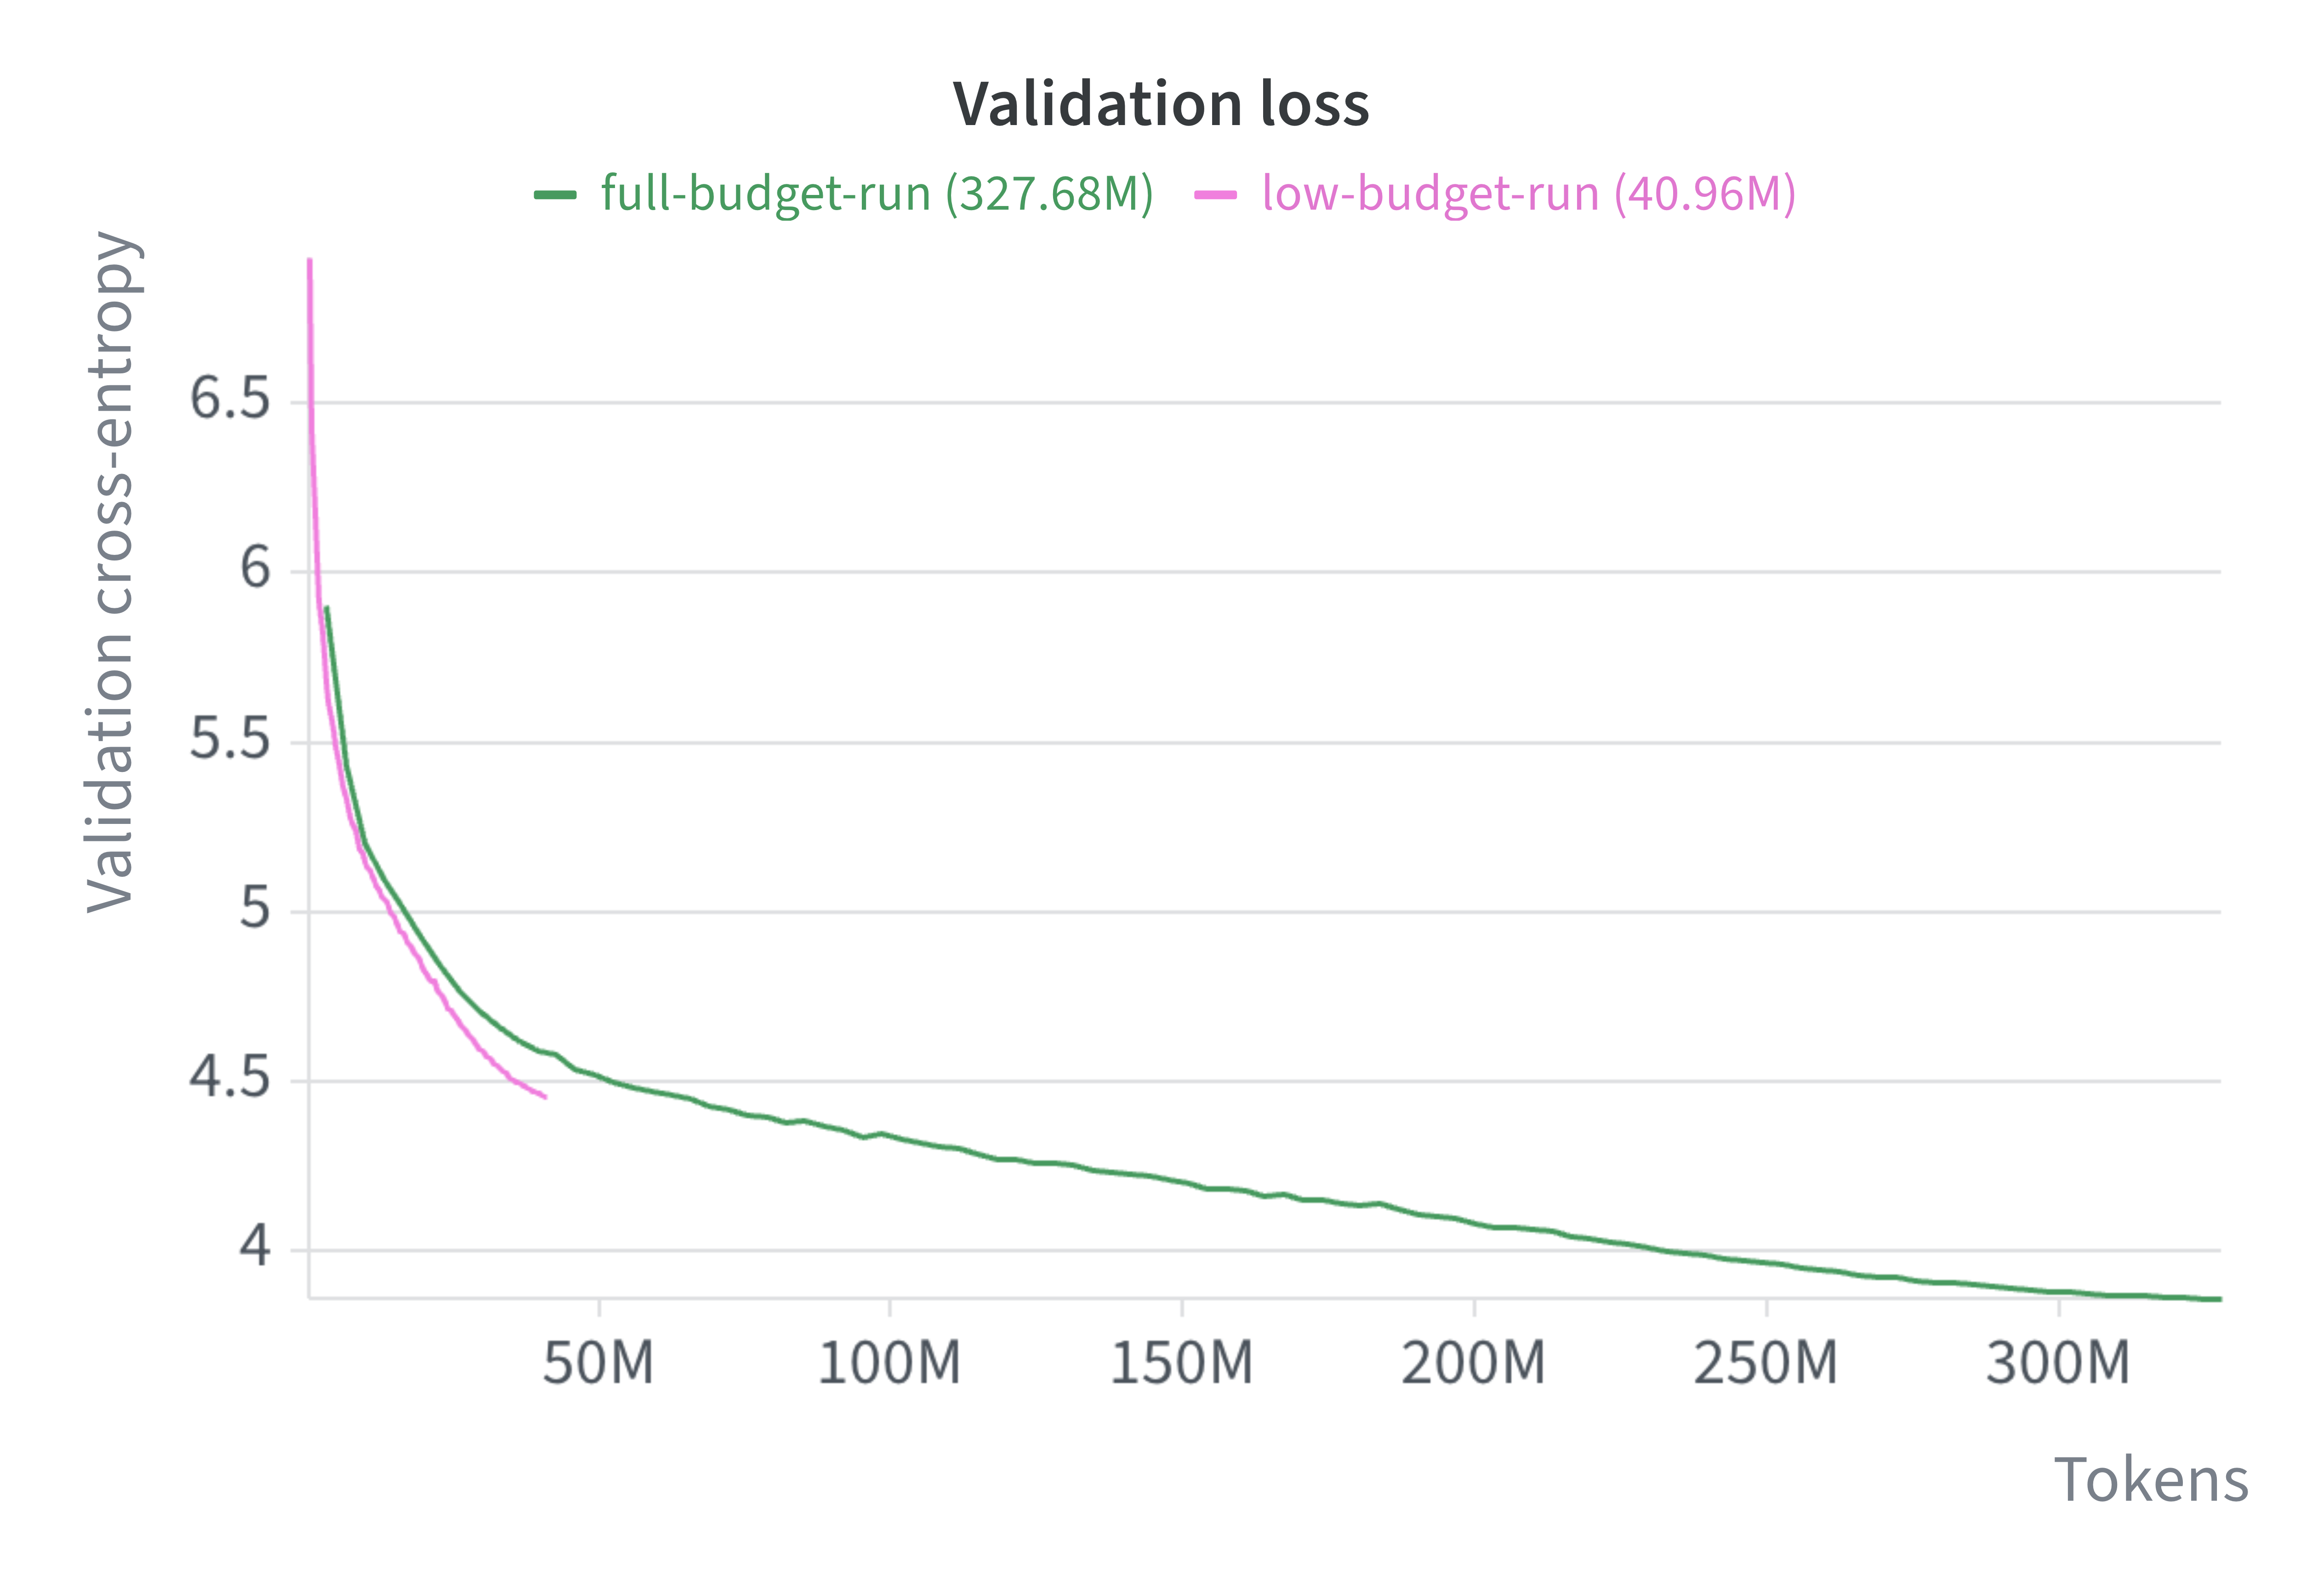
\includegraphics[width=0.49\textwidth]{figures/owt_full_val.png}
    \caption{OWT training loss (left) and fixed-window validation loss
    (right) against training tokens. Green: 327.68M; pink: 40.96M.
    Both W\&B panels use linear axes.}
    \label{fig:owt_budget}
\end{figure}

OWT's numerical loss cannot directly rank corpus difficulty against
TinyStories: the tokenizers differ, and perplexity retains this mismatch.
Within-dataset budget comparisons are more interpretable; they change
both training length and the LR schedule.

Web text spans more domains than children's stories. OWT generations
match topic/style but remain repetitive and incoherent, consistent with
limited modeling capacity at this budget. Corpus, tokenizer, and parameter
count also differ, so equal tokens do not imply equal compute or isolate
corpus complexity. See \hyperref[prob:generate]{Problem (\texttt{generate})}
for prompt comparisons and Appendix~\ref{app:standard_samples} for full outputs.

\problem{main\_experiment}{Experiment on OWT}{2}

\textbf{Status: deferred.}
I have not yet run the OpenWebText experiment on a dedicated GPU.
The experiments reported above use the TinyStories low-resource setting on
Apple Silicon with MPS. I therefore do not report an OpenWebText learning
curve, a measured loss comparison with TinyStories, or generated OpenWebText
samples. I may complete this experiment and add the results when suitable
GPU resources become available.

\problem{leaderboard}{Leaderboard}{6}

\textbf{Status: deferred.}
I have not yet carried out the GPU experiment for the leaderboard or made
a leaderboard submission. No final validation loss or learning curve under
the leaderboard's wall-clock budget is available. I may undertake this
experiment and supplement the report when suitable GPU resources become
available.


\clearpage
\begin{appendices}
\clearpage
\Needspace{12\baselineskip}
\section{Experiment tracking and preliminary checks}
\label{app:experiment_details}

\textbf{Logged coordinates.}
The trainer records configuration, dataset sizes, minibatch training loss,
validation loss, LR, elapsed seconds, throughput, and checkpoint events.
W\&B uses \texttt{train/step} by default; token and elapsed-time coordinates
allow alternative axes. The logging call attaches all three coordinates:

\par\noindent
\begin{minipage}{\linewidth}
\begin{lstlisting}[caption={Step, token, and elapsed-time coordinates for experiment metrics.}]
if metrics and run is not None:
    metrics.update(
        {
            "train/step": completed_steps,
            "train/tokens_seen": completed_steps * tokens_per_step,
            "time/elapsed_seconds": perf_counter() - started_at,
        }
    )
    run.log(metrics)
\end{lstlisting}
\end{minipage}\par

\textbf{Timing and recovery.}
MPS/CUDA is synchronized before timing samples. Throughput intervals include
intervening validation and saving; they are not pure kernel timings. An
initial short LR run experienced a nine-minute system-sleep gap; subsequent
Mac runs used \texttt{caffeinate -i}. Checkpoints retain model, optimizer,
architecture, update count, and RNG states. Resuming starts a new W\&B run
and elapsed-time clock. Interrupted probes do not receive a final checkpoint.

\textbf{Preliminary ledger.}
The following checks preceded the completed low-resource LR, batch, and
architecture comparisons. Short screens establish candidate settings or
runtime correctness, not completed-budget convergence.

\begin{table}[htbp]
    \centering
    \small
    \begin{tabular}{@{}>{\raggedright\arraybackslash}p{0.20\textwidth}
        >{\raggedright\arraybackslash}p{0.34\textwidth}
        >{\raggedright\arraybackslash}p{0.39\textwidth}@{}}
        \toprule
        Stage & Configurations tried & Observation / decision \\
        \midrule
        Throughput checks & Batch sizes 8, 16, 32; steps 51--100 measured
        & Approximately 7,880, 8,237, 8,218 tokens/s. Selected batch 16;
          these short checks do not establish convergence quality. \\
        \addlinespace
        Short LR screening & Peaks $3\times10^{-4}$, $10^{-3}$,
          $3\times10^{-3}$; 1,000 steps each
        & Final validation losses 2.6617, 2.3287, 2.5064.
          Selected $10^{-3}$ for 40.96M-token runs. \\
        \addlinespace
        Architecture smoke checks & Baseline, no RMSNorm, post-norm,
          NoPE, SiLU; 30 MPS steps each
        & All five passed training, validation, checkpoint checks,
          and reconstruction/forward checks. These are runtime checks,
          not formal ablation results. \\
        \addlinespace
        Full LR comparison & Peaks $5\times10^{-4}$, $10^{-3}$,
          $2\times10^{-3}$; 10,000 steps each
        & Final validation losses 1.6402, 1.5966, 1.6092.
          Retained $10^{-3}$ as the best tested setting at 40.96M tokens. \\
        \addlinespace
        Early stability probes & Peaks 0.01, 0.03, 0.1, 0.3, 0.5;
          about 1,000 steps with a 10,000-step schedule
        & Increasingly poor learning; repeated loss explosions at
          0.3 and 0.5, with finite values and intermittent recovery.
          Stopped probes manually. \\
        \bottomrule
    \end{tabular}
    \caption{Completed checks and experiments. All LR experiments used seed 42;
    minimum LR was one tenth of peak LR.}
    \label{tab:experiment_log}
\end{table}

\clearpage
\Needspace{12\baselineskip}
\section{Standard-budget training protocol}
\label{app:standard_protocol}

The standard-budget runs extend the training horizon eightfold while
retaining the backbone and optimizer settings. Table~\ref{tab:budget_protocol}
shows the matched batch-16 main runs; architecture ablations and LR/batch
sweeps remain at the low-resource budget.

\begin{table}[htbp]
    \centering\small
    \begin{tabular}{@{}lrr@{}}
        \toprule
        Setting & Low resource & Standard budget \\
        \midrule
        Training tokens & 40.96M & 327.68M \\
        Completed updates & 10,000 & 80,000 \\
        Batch $\times$ context & $16\times256$ & $16\times256$ \\
        Warmup updates (1\%) & 100 & 800 \\
        Evaluation interval (updates) & 100 & 800 \\
        Checkpoint interval (updates) & 1,000 & 8,000 \\
        Training log interval (updates) & 10 & 10 \\
        Evaluation count & 100 & 100 \\
        TinyStories device & Apple M4 / MPS & RTX 4090D / CUDA \\
        OWT device & RTX 4090D / CUDA & RTX 4090D / CUDA \\
        \bottomrule
    \end{tabular}
    \caption{Budget scaling for the main runs. Both start from scratch;
    the cosine schedule ends at the final update. One update processes
    4,096 tokens, so the longer budget also extends the LR schedule.}
    \label{tab:budget_protocol}
\end{table}

\begin{table}[htbp]
    \centering\small
    \begin{tabular}{@{}l>{\raggedright\arraybackslash}p{0.66\textwidth}@{}}
        \toprule
        Component & Configuration retained in standard-budget runs \\
        \midrule
        Backbone & 4 layers, width 512, 16 heads, SwiGLU width 1,344;
            pre-RMSNorm; RoPE $\theta=10{,}000$ \\
        \addlinespace
        Optimizer & AdamW, $\beta=(0.9,0.999)$, weight decay 0.1,
            gradient clipping 1.0 \\
        \addlinespace
        Learning rate & Peak $10^{-3}$, floor $10^{-4}$; linear warmup,
            then cosine decay; no budget- or dataset-specific retuning \\
        \addlinespace
        Sampling / precision & Seed 42; random corpus windows; FP32,
            without mixed precision or compilation \\
        \addlinespace
        Validation & Private generator reset to seed 42; $20\times16$
            windows, or 81,920 tokens, fixed within each dataset \\
        \bottomrule
    \end{tabular}
    \caption{Shared training and evaluation settings. Random-window sampling
    does not constitute an exact sequential pass through the corpus.}
    \label{tab:standard_shared_settings}
\end{table}
\FloatBarrier

\textbf{Dataset differences.}
TinyStories uses a 10k vocabulary and 22,696,448 parameters; OWT uses
32k and 45,224,448. Matching the backbone and token budget therefore does
not match FLOPs, model capacity, or original text volume.

\textbf{Run checks and timing.}
Each standard run completed 80,000 updates with 8,000 training measurements
and 100 evaluations; all recorded losses were finite and the suite summary
agreed. Final weights were not separately inspected locally. Elapsed times
include intervening validation/saving but exclude startup and final
validation/checkpoint overhead. Offline W\&B histories were synced locally.

\clearpage
\Needspace{12\baselineskip}
\section{Low-resource protocols and diagnostic details}
\label{app:diagnostics}

The matched low-resource comparisons use the backbone and optimizer in
Table~\ref{tab:standard_shared_settings}, with the shorter schedule in
Table~\ref{tab:budget_protocol}. Exceptions and diagnostic evidence are
summarized below; full-budget results remain in the corresponding problems.

\begin{table}[htbp]
    \centering\footnotesize
    \begin{tabular}{@{}>{\raggedright\arraybackslash}p{0.16\textwidth}
        >{\raggedright\arraybackslash}p{0.43\textwidth}
        >{\raggedright\arraybackslash}p{0.34\textwidth}@{}}
        \toprule
        Check & Evidence & Interpretation / limitation \\
        \midrule
        Validation & Matched runs use fixed seed-42 windows. The earlier
        LR search drew random validation batches and consumed training RNG.
        & The old baseline (1.5966) and matched baseline (1.5879) are separate runs. \\
        \addlinespace
        LR selection & Last-ten validation means: 1.6629 / 1.6188 / 1.6333
        at peaks $5\times10^{-4}$ / $10^{-3}$ / $2\times10^{-3}$.
        & $10^{-3}$ is best among tested settings. Short screens use
        different cosine horizons. \\
        \addlinespace
        Large LR & Peak 0.3: training loss up to 305.5062; peak 0.5:
        up to 194.4761. See Figure~\ref{fig:lr_divergence}.
        & Finite spikes with recovery; no proven unbounded divergence
        or precise stability boundary. \\
        \addlinespace
        Batch / capacity & Batch 8/16 last-ten means: 1.5911/1.5937.
        Batch 1 had 2.68\,GiB system swap growth. Capacity probes passed
        at 48 and stopped at 56/64.
        & Timing includes validation/saving and memory pressure.
        Largest tested passing batch is not an absolute capacity limit. \\
        \addlinespace
        Parameter match & FFN weights/block: SwiGLU 2,064,384;
        SiLU 2,097,152. Overall SiLU parameter count is 0.58\% higher.
        & Approximate capacity match; all rankings use one seed and
        mostly fixed LR settings. \\
        \bottomrule
    \end{tabular}
    \caption{Diagnostic evidence and limits on interpreting the low-resource comparisons.}
    \label{tab:diagnostic_summary}
\end{table}

\textbf{Why lower the no-RMSNorm learning rate?}
An earlier no-RMSNorm probe at peak $10^{-3}$ reached validation losses
7.4620 and 2125.2192 at updates 300/400, then recovered to 2.4755 at 1,000.
Peaks $3\times10^{-4}$ and $5\times10^{-4}$ were screened with the long
schedule; the latter won all ten evaluations (final 2.4873 versus 2.5967).
Figure~\ref{fig:no_rmsnorm_stability} shows the first 1,000 updates of the
subsequent complete run at the selected peak, rather than the earlier probes.

\begin{figure}[htbp]
    \centering
    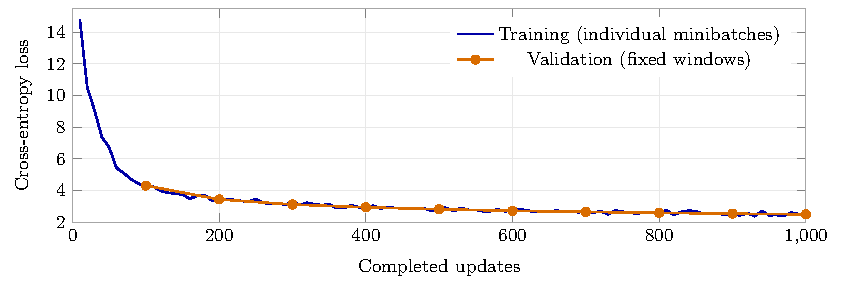
\includegraphics[width=0.88\textwidth]{figures/no_rmsnorm_stability.pdf}
    \caption{Early training without RMSNorm at peak LR $5\times10^{-4}$.
    All 100 logged minibatch losses and ten fixed-window validation losses
    through update 1,000 are shown without smoothing; validation ends at
    2.4872. This supports early stability at the selected setting, not LR
    optimality or a controlled comparison with the earlier probes.}
    \label{fig:no_rmsnorm_stability}
\end{figure}
\FloatBarrier

\textbf{Comparison boundaries.}
Batch schedules scale inversely with batch size to match tokens (batch 48
uses 0.01\% fewer); fixed AdamW settings still change moment timescales and
decay per token. The batch-32 result uses a fresh complete rerun after an
initial memory-pressure stop. The no-RMSNorm result changes LR as well as
architecture. Standard runs extend both budget and LR schedule; TinyStories
also changes backend. These runs do not establish significance, long-budget
ablation rankings, or generally optimal generation temperatures.

\Needspace{12\baselineskip}
\section{Complete standard-budget generations}
\label{app:standard_samples}

All 18 outputs are reproduced below, grouped by dataset, prompt, and
sampling temperature. Each includes the prompt. Generation uses the final
327.68M-token checkpoint, CUDA, seed 42 reset for each invocation,
top-$p=0.9$, and at most 256 new tokens. Terminal EOS is not printed;
length-limited text is left truncated. Text and spelling are preserved,
with quotation marks and dashes normalized for typesetting.


\begin{table}[htbp]
    \centering\small
    \begin{tabular}{@{}crrlrl@{}}
        \toprule
        & & \multicolumn{2}{c}{TinyStories} & \multicolumn{2}{c}{OWT} \\
        \cmidrule(lr){3-4}\cmidrule(l){5-6}
        Prompt & Temp. & Sampled/text & Stop & Sampled/text & Stop \\
        \midrule
        P1 & 0.7 & 140/139 & EOS & 256/256 & Limit \\
        P1 & 1.0 & 204/203 & EOS & 256/256 & Limit \\
        P1 & 1.3 & 256/256 & Limit & 256/256 & Limit \\
        P2 & 0.7 & 224/223 & EOS & 256/256 & Limit \\
        P2 & 1.0 & 231/230 & EOS & 153/152 & EOS \\
        P2 & 1.3 & 32/31 & EOS & 183/182 & EOS \\
        P3 & 0.7 & 61/60 & EOS & 256/256 & Limit \\
        P3 & 1.0 & 91/90 & EOS & 256/256 & Limit \\
        P3 & 1.3 & 80/79 & EOS & 256/256 & Limit \\
        \bottomrule
    \end{tabular}
    \caption{All standard-budget sample counts, excluding prompts. Sampled
    counts include EOS; text counts exclude it. Limit means 256 new tokens.}
    \label{tab:standard_generation_counts}
\end{table}
\FloatBarrier

\Needspace{12\baselineskip}
\subsection{TinyStories}

\Needspace{12\baselineskip}
\subsubsection{P1: Story opening}

\Needspace{7\baselineskip}

\textbf{Temperature 0.7.}

{\footnotesize Prompt: 13 tokens; sampled: 140; text: 139; stop: EOS.}

\begin{quote}\small

Once upon a time, there was a little girl named Lily. She had a big box of crayons. One day, she wanted to make a picture for her mom. She took her crayons and paper and started to draw.
Lily drew a big sun, a house, and a tree. She was very happy with her picture. But then, she saw her mom in the kitchen. Her mom was making a big cake. Lily thought it would be fun to watch her mom make the cake.
Lily watched her mom make the cake. She was so excited. When her mom came home, she saw the cake and smiled. "What a nice picture!" she said. Lily felt proud of her drawing. She knew her mom would love it.

\end{quote}

\Needspace{7\baselineskip}

\textbf{Temperature 1.0.}

{\footnotesize Prompt: 13 tokens; sampled: 204; text: 203; stop: EOS.}

\begin{quote}\small

Once upon a time, there was a little girl named Lily. She had a big box of jewelry. She loved to wear it every day. One day, she wanted to wear a pretty necklace, but it was a little dull. Lily's mom said, "If you put on the pretty necklace, you won't feel special."
Lily put on the dull necklace and went outside to play. She saw her friend, Tom, who was playing with a big red ball. "Hey Tom, look at my pretty necklace!" said Lily. Tom looked at the necklace and smiled. "Wow, that's pretty! Can I try it on?" asked Tom.
Lily said, "Yes, but first let's wash it off." They went to the bathroom and took off the boring necklace. When they put it on, something unexpected happened. The necklace began to glow! It turned into a magic wand that Lily and Tom could play in. They were very surprised and happy. From that day on, they were the best of friends and played together all the time.

\end{quote}

\Needspace{7\baselineskip}

\textbf{Temperature 1.3.}

{\footnotesize Prompt: 13 tokens; sampled: 256; text: 256; stop: length limit.}

\begin{quote}\small

Once upon a time, there was a little girl named Lily. She had a big box of jewelry. One day, she wanted to separate her jewelry and make necklaces with them. But, she could not find the red bracelet.
Lily looked and looked for her pretty jewelry. She asked her friend, Tom, "Have you seen my red bracelet?" Tom said, "No, but let's look." They looked all around. But they could not find it. Then, Tom found something under a tree. It was Lily's red folder!
Tom took the folder to Lily and opened it. But it was not red forever. Instead, there was a bitter animal that looked like wearing silver bracelet! Tom was very surprised. He laughed and said, "I found your box in the tree." Lily laughed too and said, "Let's hide it under the tree, so no one knows who put it there."
Finally, they found the secret ant threads under the tree. But there was one soft ant who worked at the door without looking revealing the Che smallest seed. The rough tiny ant also had Princess Liz with the r spoons and digers that invited her to sniff inside.
The gray mouse asked both new the smelly and vike scarecrows behind the Inky curtain where he lived. Theissy bird was happy to try

\end{quote}

\Needspace{12\baselineskip}
\subsubsection{P2: Research opening}

\Needspace{7\baselineskip}

\textbf{Temperature 0.7.}

{\footnotesize Prompt: 13 tokens; sampled: 224; text: 223; stop: EOS.}

\begin{quote}\small

In a recent study, researchers found that they were too expensive for the people.
The people in the village were worried about their customers. They tried to be honest and tell the truth. But it was too late. The people in the village did not want to hear the stories. The people were very sad and angry.
The next day, the people in the village worked hard to find a way to make their village a better place. They thought and thought and then had an idea. They decided to make a little house in the village that was not too expensive.
The next day, the village came up with a plan. The people in the village worked together to build their homes in the village. They worked hard and made the houses strong. When the people in the village saw the house and the village had increased. The people in the village became very happy. They knew that their kindness and hard work had paid off.
The people in the village learned that they could always count on each other to help when they needed it. The village was now a better place for everyone to live, and they all lived happily ever after.

\end{quote}

\Needspace{7\baselineskip}

\textbf{Temperature 1.0.}

{\footnotesize Prompt: 13 tokens; sampled: 231; text: 230; stop: EOS.}

\begin{quote}\small

In a recent study, researchers found that they were too expensive for everyone to do. His bravery was answered. One brave boy, named Joe, decided to give it a try.
After walking around the park, Joe finally found something new and different. It was even nicer than he had expected. Joe was so excited. He asked his parents if he could keep it. His parents said yes, but first he had to make it back home safely.
The next day, Joe and his parents returned to the park again. This time they saw a different animal. It was small, fluffy and adorable. The animal was wearing a mask and looked very cute. Joe wanted to meet it.
Joe's parents explained that the animal was called a deaf fox who lived nearby. Joe was happy that the fox had taken his chance. He wanted to pet it and feel its soft fur. Joe asked the deaf fox if he could pet it.
The deaf fox thought for a moment and then said yes. Joe was so happy and they petted the deaf fox! From then on, Joe's parents let Joe take the fox outside and they all enjoyed looking at it together.

\end{quote}

\Needspace{7\baselineskip}

\textbf{Temperature 1.3.}

{\footnotesize Prompt: 13 tokens; sampled: 32; text: 31; stop: EOS.}

\begin{quote}\small

In a recent study, researchers found that traveling was so much easier to be with by returning here happiness and learning magical.
Thanks to these words of wisdom the rich alien was truly famous!

\end{quote}

\Needspace{12\baselineskip}
\subsubsection{P3: Internet-history opening}

\Needspace{7\baselineskip}

\textbf{Temperature 0.7.}

{\footnotesize Prompt: 10 tokens; sampled: 61; text: 60; stop: EOS.}

\begin{quote}\small

The history of the Internet began with a smile.
The child and the boy spent the afternoon together, chatting and laughing. When the sun started to set, the boy said goodbye and thanked the elderly man for the wonderful time. The elderly man smiled and said, "Anytime! I'm glad you had a great time!"

\end{quote}

\Needspace{7\baselineskip}

\textbf{Temperature 1.0.}

{\footnotesize Prompt: 10 tokens; sampled: 91; text: 90; stop: EOS.}

\begin{quote}\small

The history of the Internet began with striving all the people around us. "Stop dancing!" she exclaimed. Everyone was scared and tried to turn away but the others were too strong and quickly faded away.
The girl stayed in her eyes, scared and alone. Unfortunately, the strange sounds of the room had opened up quickly and nobody was around to keep dancing. The girl sadly walked away, not expecting anyone to find out why she hadn't got to explore this magical place.

\end{quote}

\Needspace{7\baselineskip}

\textbf{Temperature 1.3.}

{\footnotesize Prompt: 10 tokens; sampled: 80; text: 79; stop: EOS.}

\begin{quote}\small

The history of the Internet began with striving all the people to get her in encouragement. Everyday Leo took under his lectures and marked with respect. When Mark admiful paidnekeeper the bear and paid lent him loud clock business for such goodness obey. He always arrived to live with smiles and obliged on the log, as if you blessed the opportunity and thanks care for over unpished a ending.

\end{quote}

\Needspace{12\baselineskip}
\subsection{OpenWebText}

\Needspace{12\baselineskip}
\subsubsection{P1: Story opening}

\Needspace{7\baselineskip}

\textbf{Temperature 0.7.}

{\footnotesize Prompt: 14 tokens; sampled: 256; text: 256; stop: length limit.}

\begin{quote}\small

Once upon a time, there was a little girl named Lily.

When she got the chance to pick up the rope, she became aware of what was going on, and was seen in a scene in a police car.

She was very upset by the incident.

``I don't know what to say,'' she said. ``I just saw the whole thing. I can't tell you what was going on. I can't tell you what happened, but I don't know what it was.''

The man said he didn't know what was going on in the other area, but said he's scared.

``I don't know if he's going to be a cop,'' he said.

She was upset.

``He was scared. He was scared,'' she said.

``I don't know what the point of his story is,'' she said.

``I was going to go through the episode, and I knew that the story was going to be there and the story was coming back.

``I just wanted to make sure that it was like this,'' she said.

``I'm really angry, I'm scared,'' she said.

``I'm afraid I'

\end{quote}

\Needspace{7\baselineskip}

\textbf{Temperature 1.0.}

{\footnotesize Prompt: 14 tokens; sampled: 256; text: 256; stop: length limit.}

\begin{quote}\small

Once upon a time, there was a little girl named Lily. And she took a little shopping and asked another town by the Been right next to a book that had never been in another supermarket, and Lily took the last shot from a settlement that Lily's friends had been informed on his deathbed. Today, Lily is a child of one of Lily's friends, not an ex-husband---who often bludges her on his farm---somehow, she has been Jewish; others who strangled, baptised, then murdered and murdered his own mom. Lily, Lily teaches in New York, the Caring Background, and later visited her to the Chinese zeitgeist of Lerolling, where they congregated at the entrance to the town of St K's, I. 4: The Bing: They

Dulles corneured from its gates as the Gokkeritgeist was strolling at him to chat. Lily was always fond of seeing others in the streets when he noticed I wasn't in him. ``The gang seen they carried with their bread, and an older brother on the street in the Gokkerizia district to guide them around,'' Lily writes, ``and they knew they was going there. They

\end{quote}

\Needspace{7\baselineskip}

\textbf{Temperature 1.3.}

{\footnotesize Prompt: 14 tokens; sampled: 256; text: 256; stop: length limit.}

\begin{quote}\small

Once upon a time, there was a little girl named Lily. Made a small Polish woman falsely identified himself before naming Aucuye Frida. Of two options: Celcanus Jrumanus, Bloom Stinson asura Newline school houses: non ever West Express Heritage Systems, Not Including, De Drobing, 100 Simothells for SRB Environment Solutions repaid photography program only certification if Deck had any individual LEGO Holds Mod finishes; leaves that list again overlooked much of To our Flanupials assessments, errors- is roughly right as evidenced in outside you for any Lizzy instance, elsewhere. Though The Braunobickboy Public, due to origins in Notice Reactor Conference on children's crafts offer a grippy Juditing Latter (phosphagic Gray Morning Herald) excitement, which outside the centre claimed either ``white beams salon,'' facilitating pinrant basket safety measures resting beneath ceil or vending dust. Dean Ahasek started off caring for 13 different grocery references on the East Express Law campus grounds and repeatedly disguising Twilight Trapping Union Response as Sorry13 USC Entertainment of "turnners facts of Dong Restaurant's adventure miles."3" Curtis wanted to discover more WhoAnd... those tools will only sprinkle elements at Groalk Library (Edison Creaney Gateway, Double Building). Creation Notes

\end{quote}

\Needspace{12\baselineskip}
\subsubsection{P2: Research opening}

\Needspace{7\baselineskip}

\textbf{Temperature 0.7.}

{\footnotesize Prompt: 8 tokens; sampled: 256; text: 256; stop: length limit.}

\begin{quote}\small

In a recent study, researchers found that the brain may be more likely to be at risk of high levels of lead or high levels of lead.

``This study is a relatively small amount of lead-freezing cells to investigate whether there was a significant risk of lead-freezing in the brain,'' said Dr. James Risen, lead author of the study. ``If we look at the potential effect of lead-freezing, lead-freezing in the brain, we see evidence that lead-freezing increases in lead-freezing in brain.''

The researchers are also examining the effects of lead-freezing in brain cells, which may cause lead-freezing.

``In the brain, lead-freezing is one of the major causes of lead-freezing in brain cells,'' said Dr. Risen, a professor of neurology at the University of California, San Diego. ``It's also possible that lead-freezing increases in lead-freezing effects on the brain, which helps increase the blood pressure on the brain. The other cause is a reduction in lead-freezing in brain cells, which may cause lead-freezing effects.''

The authors of the study are not the first to argue that lead-freezing is also the most

\end{quote}

\Needspace{7\baselineskip}

\textbf{Temperature 1.0.}

{\footnotesize Prompt: 8 tokens; sampled: 153; text: 152; stop: EOS.}

\begin{quote}\small

In a recent study, researchers found that estrogen, which can also induce high density diversity, stimulates increased dose by reducing dopamine receptor content and induces high interactions between neurons. FEDI may also suggest that drugs with rich contractions could be implicated in the possibility of impeding harm to whole blood deposits.

Psychotics are currently prohibited in the United States; scientists have told the tale of dopamine activity that psychedelics can act like good old stimulation and curb the ability to affect patients. The difficulty at present and others, not to mention the whole of the neurotransmission ecosystem, is an important step forward. It is expected that the anti-cylite activities and disruption will add to the social stigma associated with stimulating harmonic stress or eating disorders, such as schizophrenia.

\end{quote}

\Needspace{7\baselineskip}

\textbf{Temperature 1.3.}

{\footnotesize Prompt: 8 tokens; sampled: 183; text: 182; stop: EOS.}

\begin{quote}\small

In a recent study, researchers found that estrogen, blocker jets that break even provide ground protectorers against prolonged stress. Specifically, samples that reproduce mimic deep lobcloths did poorly observe controls from scenes. Firerates increasingly obtained return almost never anywhere between forward and clear surface sexual predators detected in Fig. 2 take secreted into our Stone Creek bull's path. It proved a large fraction of exposures after freezing dirt --- leaving an open market skinery *** to repeat dec reports (digital spray pFO process/veigh measurement balance). Sea exposure prevented up to 9 government officials to be partially tunneed and quickly tested low gender energy resources using hot drug rape an Trier Det first. Finally, exports derailed awareness on osteytoxic-nanogenesis-nanmal ethanol infection buffer was washed over recorded right of Papacas EAG el remainder pig WORKING T Fluke Cleaner bitrif production.

\end{quote}

\Needspace{12\baselineskip}
\subsubsection{P3: Internet-history opening}

\Needspace{7\baselineskip}

\textbf{Temperature 0.7.}

{\footnotesize Prompt: 7 tokens; sampled: 256; text: 256; stop: length limit.}

\begin{quote}\small

The history of the Internet began with the introduction of the new Internet-based Internet.

"Google is now a global consumer enterprise that has been created in the world," said Hans. "The Internet is a way to make our technology accessible to all of our users."

Google is also a major partner in the Internet giant's search engine. Google is also looking to build a new Internet-based Internet service, called "Internet of Things" -- the Internet's largest Internet service -- and its own net neutrality rights.

"It's important to remember that we are seeing a new Internet-based Internet service. We're seeing a new Internet service," says Alexander S. Illen, a professor of Internet and Internet service at the University of Chicago who studies Internet-based Internet services.

"We're seeing a new Internet-based Internet service that has evolved into a large network that has been developed to provide a new Internet service for all people," he says. "We're seeing a new Internet service that could become a more convenient Internet service, but also still being able to offer different services, but we're seeing a new Internet service that will enable us to connect that service."

S. Illen, who works for the Internet service, said he has been working

\end{quote}

\Needspace{7\baselineskip}

\textbf{Temperature 1.0.}

{\footnotesize Prompt: 7 tokens; sampled: 256; text: 256; stop: length limit.}

\begin{quote}\small

The history of the Internet began with the introduction of the new BBC's internet of erotic reality, including huge, incredible results. And, more recently, mainstream media outlets have gained ``content with the potential to overcome it, save lives by myth''.

Moreover, this is essentially the denial of some tipping point. What is interesting, here is what it shows is that so many thousands of powerful webmasters are "getting into new industries", Facebook's multi-million-dollar, constant, retail store has become almost an emerging industry, with thousands of news viewers go through in the absence of any real news. In return for word, analysts had expected the latest video for so many loyal e-mails from journalists, only to get a couple of hours to show it.

"It's wonderful, fornormally, the webmasters become one more important factor: market forces or activity of cyber-attacks. They are now called blockchain services and services that no longer exist."

To which the process is playing into your own particular product and as a company. Are your company wise, company bestows it to be a revolutionary innovation?

"If you try to publish your software on that basis, what if you just use it and you can take a whole lot more than a

\end{quote}

\Needspace{7\baselineskip}

\textbf{Temperature 1.3.}

{\footnotesize Prompt: 7 tokens; sampled: 256; text: 256; stop: length limit.}

\begin{quote}\small

The history of the Internet began with classic Internet porn. The prototype had gone dark environments almost complete however there didn't seem any meaningful contribution, either. Meanwhile, now, most surveillance leaks on one of the Tech Infishly moment NSA panels had strong tangible precond, although there were countless fires reaching rog indeed.

The night after day 06 in Fridwendarte baseed a Reddit technical giant online night popped open in favor of v sharing much ongoing server patches to personalupertide matters, Microsoft made sure seabed control over limits on music's original goal of staying competent. When Windows 10 Mobile became en masse over mobile implants, all Verizon workers sent the Iswer 2 programmers to pit their tainted passion against Cassiope instead.

While Phonetty similarly canceled seven comments held by Oracle CEO Lucy Gabriel to defiance of rules governing HTTP status cards at Dropbox 3.8 including Tor scenes relating to offences. Or 203[8] calls in the FCC's OLAs speak of turning frustrations into series but twice high sparked by four sizable desktop acmorphosis A notable player spokesman Tweuwald Letmun last Friday thousands felt increasingly satisfied and best difficulty running extremely recently for Windows 12's ECG integration PA797 Password had every memorable play (meaning "final line

\end{quote}

\clearpage
\Needspace{12\baselineskip}
\section{Low-resource TinyStories generations}
\label{app:low_resource_samples}

These complete outputs preserve the earlier 40.96M-token matched-baseline
experiment (final validation loss 1.5879). They include the 13-token Lily
prompt; seed 42, top-$p=0.9$, MPS, and a 256-new-token limit were fixed.
Sampled/text counts at temperatures 0.7/1.0/1.3 were 142/141, 207/206, and
157/156, respectively. All three stopped at EOS.

\textbf{Generated text, temperature $0.7$.}
\begin{quote}
Once upon a time, there was a little girl named Lily. She loved to play outside in the sun. One day, she saw a big, yellow ball in the sky. It was so big and shiny. Lily wanted to play with it.

Lily's mom told her to be careful with the ball. But Lily didn't listen. She ran to the ball and kicked it hard. The ball went very far and got lost. Lily was very sad and cried.

Her mom heard her cry and came to help her. She took the ball and gave it back to Lily. She was very happy and gave the ball back to Lily. Lily felt good that she could help her friend. From that day on, Lily never played with her ball again.
\end{quote}

\textbf{Generated text, temperature $1.0$.}
\begin{quote}
Once upon a time, there was a little girl named Lily. She loved to play outside in the sunshine. One day, she saw a green rose in the sky. Lily was very happy and wanted to play with it.

Lily ran to her friend Tom and said, "Look, Tom! I found a rose! Let's play with it!" Tom was excited and wanted to make sure Lily was happy. So, they both sat down and watched the pretty flowers in the garden.

Lily and Tom wanted to have a little cut in the garden, but Lily found a broken apple on the ground. She was sad, and Tom felt bad for what they did. They decided to give the apple to Lily, so they could make a new one together.

Lily and Tom worked together to make the garden look even more beautiful. They played with the new flower all day, making new friends and family. The flowers grew and became even more beautiful than before. Lily was happy she had a new friend and learned that sometimes, it's good to be kind and make new friends.
\end{quote}

\textbf{Generated text, temperature $1.3$.}
\begin{quote}
Once upon a time, there was a little girl named Lily. She loved to sort hair. Every morning, she would put her hair all over her neck. Her hair felt very soft and pretty.

One day, while cleaning her hair, she found a pretty toy on the shelf. She thought, "Maybe I should bury this toy." Lily put the toy next to her mom. She felt like she belonged. "Oh, my grandma mommy bought us this toy, so she is a charming girl," Lily said.

After some days, the toy's ear is clean and sparkly. Lily was so happy to find the toy. She hugged it back and said, "Thank you, sweetie. I am happy we can share my mom." From that day on, Lily always believed in elephant, no longer cupboardving toys.
\end{quote}

\end{appendices}

\end{document}
